\documentclass[11pt]{article}

\usepackage{amsthm}
\usepackage{amssymb}
\usepackage{amsmath}
\usepackage{cite}
\usepackage{hyperref}
\usepackage{mathtools}
\usepackage{subcaption}
\usepackage{tikz}
\usepackage{float}
\usepackage{caption}
\usepackage[nottoc]{tocbibind}
\usepackage[english]{babel}
\usepackage[utf8x]{inputenc}
\usepackage{venndiagram}
\usepackage{xspace}
\usepackage{centernot}
\usepackage[linesnumbered,ruled,lined,boxed,vlined,noend]{algorithm2e}
\usepackage[[deletedmarkup=xout, commentmarkup=footnote]{changes}

\newcommand{\accente}{\`E }

\newcommand{\splitfunc}{\textup{Split}}
\newcommand{\rankfunc}{\textup{rank}}
\newcommand{\rankfuncnomath}{\emph{rank}\xspace}
\newcommand{\rscp}{\textup{RSCP}}
\newcommand{\rscpnomath}{\emph{RSCP}\xspace}
\newcommand{\prefunc}{\textup{Pre}}
\newcommand{\prefuncnomath}{\emph{Pre}\xspace}
\newcommand{\succfunc}{\textup{Succ}}
\newcommand{\succfuncnomath}{\emph{Succ}\xspace}

\makeatletter
\renewcommand{\boxed}[1]{\text{\fboxsep=.2em\fbox{\m@th$\displaystyle#1$}}}
\makeatother

\newcommand\restr[2]{{% we make the whole thing an ordinary symbol
  \left.\kern-\nulldelimiterspace % automatically resize the bar with \right
  #1 % the function
  \vphantom{\big|} % pretend it's a little taller at normal size
  \right|_{#2} % this is the delimiter
  }}

\newcommand\sccto{\stackrel{\mathclap{\normalfont\mbox{\tiny{SCC}}}}{\to}}
\newcommand\superscc{\scalebox{.5}{SCC}}

\definechangesauthor[name=Alberto Casagrande, color=red]{ac}

\usetikzlibrary{arrows,automata,patterns,shapes,snakes,arrows.meta}

\graphicspath{ {imgs/} }

\captionsetup[figure]{name=Figura}
\captionsetup[table]{name=Tabella}
\renewcommand{\algorithmcfname}{Algoritmo}
\renewcommand\labelitemi{--}

\SetArgSty{textnormal}

\theoremstyle{definition}
\newtheorem{definition}{Definizione}[section]
\newtheorem{example}{Esempio}[section]
\newtheorem{axiom}{Assioma}[section]
\newtheorem*{axiom*}{Assioma}
\newtheorem{observation}{Osservazione}[section]
\newtheorem*{observation*}{Osservazione}

\theoremstyle{plain}
\newtheorem{proposition}{Proposizione}[section]
\newtheorem{lemma}{Lemma}[section]
\newtheorem{theorem}{Teorema}[section]
\newtheorem{corollary}{Corollario}[section]

\newcommand{\notimplies}{\mathrel{{\ooalign{\hidewidth$\not\phantom{=}$\hidewidth\cr$\implies$}}}}

\newenvironment{proof2}
{
  \begin{proof}[Dimostrazione]
}
{\end{proof}}

\includeonly{sezione3/file}

\begin{document}

\renewcommand\contentsname{Indice}
\tableofcontents
\addtocontents{toc}{~\hfill\textbf{Pagina}\par}

\section{Nozioni di Base}
\label{sec:base}

\subsection{Relazioni Binarie}
Riportiamo la definizione di \emph{relazione binaria} su uno o due insiemi, che sarà utile per definire formalmente il concetto di \emph{grafo}, fondamentale all'interno di questo elaborato:
\begin{definition}
    Una \emph{relazione binaria} su $A,B$ è un sottoinsieme del prodotto cartesiano $A \times B$.\\
    Una \emph{relazione binaria} su $A$ è un sottoinsieme del prodotto cartesiano $A \times A$.\\
	Se $R$ mette in relazione $u,v$, cioè $(u,v) \in R$, si usa la notazione $u R v$.
\end{definition}
\begin{definition}
    L' \emph{insieme immagine} di un elemento $x$ dell'insieme $A$ attraverso la relazione $R$ è l'insieme $R(x) = \{y \in B \mid x R y\}$.
\end{definition}
Alcune relazioni binarie mostrano proprietà fondamentali, che presentiamo nella definizione seguente:
\begin{definition}
    Sia $R$ una relazione binaria su $A$. $R$ è:
    \begin{itemize}
        \item \emph{Riflessiva} se $\forall x \in A, x R x$;
        \item \emph{Simmetrica} se $x R y \implies y R x \,\,(x,y \in A)$;
        \item \emph{Transitiva} se $(x R y \land y R z) \implies x R z \,\,(x,y,z \in A)$.
    \end{itemize}
\end{definition}
\begin{example}
    La relazione ``$\leq$'' sui naturali è riflessiva e transitiva, ma non simmetrica.\\
    La relazione ``$=$'' ($a = b \iff $``$a,b$ sono lo stesso numero'') sui naturali è simmetrica, riflessiva e transitiva.
\end{example}
\begin{definition}
    E' una \emph{relazione di equivalenza} una relazione binaria riflessiva, simmetrica e transitiva. Questo genere di relazione divide un insieme in \emph{classi di equivalenza} all'interno delle quali tutte le coppie di elementi sono in relazione.\\
    Data una relazione di equivalenza $R$ su un insieme $A$, si usa la notazione ``$[a]_R, a \in A$'' per indicare la classe di equivalenza di $R$ a cui appartiene $a$.\\
    Inoltre si usa la notazione ``$A/R$'', che si legge ``\emph{quoziente} di $A$ rispetto a $R$'', per denotare l'insieme delle classi di equivalenza di $R$ su $A$.
\end{definition}
In alcune situazioni risulta conveniente definire la più piccola relazione che dispone di una certa proprietà, e che contiene una relazione binaria $R$. Una relazione costruita in questo modo è una ``\emph{chiusura}'':
\begin{definition}
	Sia $R$ una relazione binaria su $A$. Le seguenti relazioni sono chiusure di $R$:
    \begin{itemize}
        \item \emph{Riflessiva}: $R_r = R \cup \{(x,x) \mid x \in A\}$
        \item \emph{Simmetrica}: $R_s = R \cup \{(y,x) \mid x R y\}$
        \item \emph{Transitiva}: $R_t = R \cup \{(x,z) \mid \exists y \in A,\, x R y \land y R z\}$
    \end{itemize}
\end{definition}
\begin{example}
    La chiusura riflessiva della relazione ``$<$'' (minore stretto) è la relazione ``$\leq$''.
\end{example}
Nel seguito useremo ampiamente la definizione seguente:
\begin{definition}
    Sia $R$ una relazione binaria su $A \times B$. La \emph{contro-immagine} di un elemento $y \in B$ rispetto ad $R$ è l'insieme $R^{-1}(y) = \{x \in A : x R y\}$.\\
    La \emph{funzione inversa} di $R$ è la funzione $R^{-1} : \mathcal{P}(B) \to \mathcal{P}(A)$, dove ``$\mathcal{P}$'' denota l'insieme delle parti, che associa ad un sottoinsieme di $B$ tutti gli $x \in A$ tali che vale $x R y$ per almeno un $y$ del sottoinsieme.
\end{definition}
Adottiamo infine la seguente notazione:
\begin{definition}
    Sia $A$ un insieme. La \emph{cardinalità} di $A$, indicata con ``$|A|$'' è il numero di elementi di $A$.\\
    Analogamente, data una relazione binaria $R$, $|R|$ è il numero delle coppie messe in relazione da $R$.
\end{definition}

\subsection{Grafi}
Con queste premesse possiamo definire un \emph{grafo} come segue:
\begin{definition}
    Sia $V$ un insieme finito non vuoto. Sia $E$ una relazione binaria su $V$. La coppia $G = (V, E)$ è un \emph{grafo diretto} (o \emph{orientato}). Con questa notazione:
    \begin{itemize}
        \item $V$ è l'insieme dei \emph{nodi} (o \emph{vertici});
        \item $E$ è una relazione binaria (in generale non simmetrica) che mette in relazione alcuni dei nodi di $G$.
    \end{itemize}
\end{definition}
\begin{example}
    \begin{figure}[t]
        \centering
        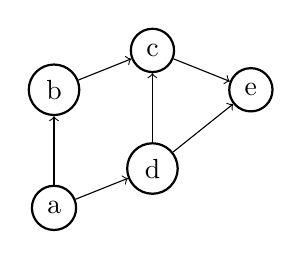
\begin{tikzpicture}[scale=0.5]
            \begin{scope}[every node/.style={circle,thick,draw}]
                \node (a) at (0,0) {a};
                \node (b) at (0,3) {b};
                \node (c) at (2.5,4) {c};
                \node (d) at (2.5,1) {d};
                \node (e) at (5,3) {e};
            \end{scope}

            \begin{scope}
                \path [->] (a) edge node {} (b);
                \path [->] (b) edge node {} (c);
                \path [->] (a) edge node {} (d);
                \path [->] (d) edge node {} (c);
                \path [->] (d) edge node {} (e);
                \path [->] (c) edge node {} (e);
            \end{scope}
            \end{tikzpicture}
        \caption{Rappresentazione grafica di un grafo diretto}
        \label{fig:graph}
    \end{figure}
    Il grafo di Figura \ref{fig:graph} è descritto dalla coppia
    \begin{itemize}
        \item $V = \{a,b,c,d,e\}$
        \item $E = \{(a,b), (a,d), (b,c), (d,c), (c,e), (d,e)\}$
    \end{itemize}
\end{example}
Nel seguito utilizzeremo ampiamente la seguente terminologia:
\begin{definition}
    Sia $G = (V,E)$ un grafo diretto. Diremo che un nodo $u \in V$ è una \emph{foglia} se $\nexists v \in V : u E v$. Diremo che $u$ è \emph{parente} di $v$ e che $v$ è \emph{figlio} di $u$ se $uEv$.
\end{definition}
Un grafo diretto è quindi un insieme di elementi (i \emph{nodi}) accoppiato con un insieme di relazioni tra questi elementi (gli \emph{archi}). \accente naturale associare questo concetto all'idea di percorso: ogni grafo è definito da un insieme di nodi ed un insieme di \emph{cammini} che consentono di spostarsi da un nodo ad un altro. La seguente definizione sorge in modo spontaneo da questa interpretazione:
\begin{definition}
    Sia $G = (V, E)$ un grafo diretto. Siano $u,v \in V$. $v$ \emph{è raggiungibile} da $u$, o in alternativa \emph{esiste un cammino} da $u$ a $v$, o ancora $u E_t v$ (la $t$ in pedice sta per ``\emph{transitivo}''), se esiste una sequenza finita di nodi $x_n$ di lunghezza $K : x_0 = u, x_K = v, x_n E x_{n+1}$.
\end{definition}
L'esistenza di un cammino tra nodi fornisce un criterio immediato per partizionare un grafo in gruppi di nodi. Diamo innanzitutto la seguente definizione:
\begin{definition}
    Diremo che un grafo diretto $(V,E)$ è \emph{fortemente connesso} se $\forall v_1, v_2 \in V, v_1 E_t v_2$.
\end{definition}
Allora possiamo individuare facilmente i sottografi massimali (cioè la ripartizione del grafo in sottografi che consente di minimizzare il numero di sottografi) fortemente connessi (\hspace*{-0.1cm}\cite[Appendice B]{clrs}):
\begin{definition}
    Le \emph{componenti fortemente connesse} (\emph{strongly connected components}, \emph{SCC}) di un grafo diretto sono i sottografi che compongono la ripartizione (massimale) del grafo in sottografi fortemente connessi.
\end{definition}
\begin{observation}
    Chiaramente i nodi contenuti in una stessa componente fortemente connessa sono mutuamente raggiungibili.
\end{observation}
\begin{example}
    \begin{figure}[t]
        \centering
        \begin{tikzpicture}[scale=0.5]
            \begin{scope}[every node/.style={circle,thick,draw}]
                \node (a) at (0,0) {a};
                \node (b) at (0,3) {b};
                \node (c) at (2.5,4) {c};
                \node (d) at (2.5,1) {d};
                \node (e)[diamond] at (5,3) {e};
            \end{scope}

            \begin{scope}
                \path [->] (a) edge node {} (b);
                \path [->] (b) edge node {} (c);
                \path [->] (d) edge node {} (a);
                \path [->] (c) edge node {} (d);
                \path [->] (d) edge node {} (e);
                \path [->] (c) edge node {} (e);
            \end{scope}
            \end{tikzpicture}
        \caption{SCC di un grafo diretto}
        \label{fig:graph_cfc_1}
    \end{figure}
    Nel grafo di Figura \ref{fig:graph_cfc_1} le SCC sono rappresentate con forme diverse: $\{a,b,c,d\}, \{e\}$.
\end{example}
Il partizionamento dei nodi in SCC è definito come segue:
\begin{definition}
    Sia $G = (V, E)$ un grafo diretto. Il grafo $G^{SCC} = (V^{SCC}, E^{SCC})$, dove:
    \begin{itemize}
        \item $V^{SCC} = \{C : \,C$ è una SCC$\}$;
        \item $E^{SCC} = \{(A,B) \in V^{SCC} \times V^{SCC} : A \neq B, \exists m \in A, n \in B : m E n\}$
    \end{itemize}
    è il partizionamento del grafo iniziale in SCC.
\end{definition}
Riportiamo la seguente proprietà immediata:
\begin{proposition}
    Sia $G^{SCC}$ il grafo delle SCC di un grafo $G$ generico. Allora $G^{SCC}$ è aciclico.
\end{proposition}
\begin{proof2}
    Supponiamo per assurdo che in $G^{SCC}$ esista un ciclo. Allora tutti i nodi di $V^{SCC}$ facenti parte del ciclo sono mutuamente raggiungibili (percorrendo il ciclo). Quindi tutti i nodi fanno parte della stessa SCC, ma questo è assurdo.
\end{proof2}
\begin{example}
    \begin{figure}[b]
        \centering
        \begin{subfigure}{.45\textwidth}
          \centering
          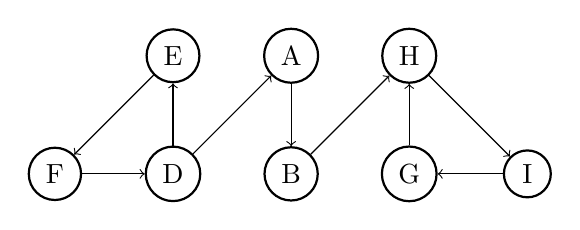
\begin{tikzpicture}[scale=0.5]
            \begin{scope}[every node/.style={circle,thick,draw}]
                \node (A) at (0,3) {A};
                \node (B) at (0,0) {B};

                \node (D) at (-3,0) {D};
                \node (E) at (-3,3) {E};
                \node (F) at (-6,0) {F};

                \node (G) at (3,0) {G};
                \node (H) at (3,3) {H};
                \node (I) at (6,0) {I};
            \end{scope}

            \begin{scope}
                \path [->] (A) edge node {} (B);

                \path [->] (E) edge node {} (F);
                \path [->] (F) edge node {} (D);
                \path [->] (D) edge node {} (E);

                \path [->] (G) edge node {} (H);
                \path [->] (H) edge node {} (I);
                \path [->] (I) edge node {} (G);

                \path [->] (D) edge node {} (A);
                \path [->] (B) edge node {} (H);
            \end{scope}
            \end{tikzpicture}
          \caption{Un grafo}
        \end{subfigure}
        \hfill
        \begin{subfigure}{.45\textwidth}
          \centering
          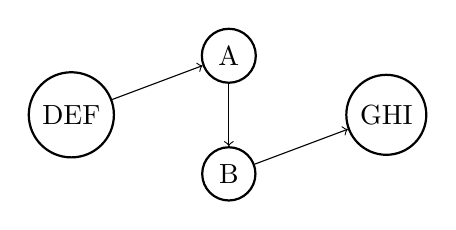
\begin{tikzpicture}[scale=0.5]
            \begin{scope}[every node/.style={circle,thick,draw}]
                \node (A) at (0,3) {A};
                \node (B) at (0,0) {B};

                \node (DEF) at (-4,1.5) {DEF};

                \node (GHI) at (4,1.5) {GHI};
            \end{scope}
                \path [->] (A) edge node {} (B);
                \path [->] (DEF) edge node {} (A);
                \path [->] (B) edge node {} (GHI);
            \begin{scope}

            \end{scope}
            \end{tikzpicture}
          \caption{Corrispondente grafo delle SCC}
        \end{subfigure}
        \caption{Un grafo ed il corrispondente grafo delle SCC}
        \label{fig:graph_cfc_2}
    \end{figure}
    La Figura \ref{fig:graph_cfc_2}.a rappresenta un grafo diretto generico, la Figura \ref{fig:graph_cfc_2}.b rappresenta il suo grafo delle componenti fortemente connesse associato.
\end{example}
Dato un grafo diretto generico possiamo determinare la partizione in SCC sfruttando un algoritmo avente complessità lineare $\Theta(|V| + |E|)$ \cite{tarjan}. L'algoritmo non verrà trattato in questo elaborato.

\subsection{Insiemi}
\subsubsection{Cenni di teoria degli insiemi}
In generale supporremo validi gli assiomi su cui si fonda la teoria degli insiemi ZFC, ad eccezione dell'Assioma di Fondazione. Diamo innanzitutto una formulazione degli assiomi che interverranno nel seguito del lavoro:
\begin{axiom}[di estensionalità]
    Due insiemi sono uguali $\iff$ contengono gli stessi elementi.
\end{axiom}
\begin{axiom}[di fondazione]
    Ogni insieme non vuoto contiene un elemento disgiunto dall'insieme stesso.
    \label{axi:foundation}
\end{axiom}
Del primo faremo un uso esplicito nel seguito. Il secondo, per motivi che saranno evidenti nella sezione seguente, risulta limitante nell'ambito trattato in questo elaborato. Introduciamo la seguente definizione:
\begin{definition}
    Un insieme è \emph{ben-fondato} se non contiene se stesso. Altrimenti è \emph{non-ben-fondato}.
\end{definition}
\begin{example}
    L'insieme $\Omega = \{\Omega\}$ è non-ben-fondato. L'insieme $A = \{1,2,3\}$ è ben-fondato.
\end{example}
Riportiamo una formulazione equivalente dell'Assioma \ref{axi:foundation}:
\begin{axiom*}[\ref{axi:foundation} bis]
    $\forall A$ la relazione ``$\in$'' è ben-fondata su $A$ \cite[Chapter III.4]{kunen}
\end{axiom*}
Da questa questa formulazione risulta evidente l'impossibilità, in ZFC, di costruire insiemi non-ben-fondati.\\
Rinunciando all'Assioma \ref{axi:foundation} si ottiene un sistema di assiomi che ammette l'esistenza di insiemi non-ben-fondati; tuttavia si può verificare che questo sistema non è più sufficiente a descrivere in modo esaustivo l'aritmetica per mezzo di operazioni su insiemi. Per ovviare a questa mancanza si introduce l'Assioma AFA, che verrà presentato e discusso nella sezione seguente.

% TODO: definisci insieme ereditariamente finito (si può costruire a partire dall'insieme vuoto utilizzando solamente il costruttore {} vedi ZFC) e insime non-ben-fondato prima di usare i grafi per rappresentare gli insiemi

\subsubsection{Rappresentazione di insiemi tramite grafi diretti}
\label{sec:graphs_sets}
In alcuni casi risulta conveniente fornire un'in\-ter\-pre\-ta\-zio\-ne insiemistica della nozione di grafo vista sopra. Introduciamo innanzitutto una nozione fondamentale:
\begin{definition}
    Sia $G = (V, E)$ un grafo orientato. Sia $u \in V : \forall v \in V, u E_t v$, cioè ogni nodo di $G$ è raggiungibile da $u$. Allora la coppia $(G, u)$ è un \emph{accessible pointed graph}, o \emph{APG}.
\end{definition}
Per rappresentare un insieme tramite un grafo diretto è necessario definire un processo denominato \emph{decorazione}:
\begin{definition}
    La \emph{decorazione} di un APG è l'assegnazione di un insieme ad ogni suo nodo. In tal caso viene associata la relazione ``$\in$'' alla relazione di raggiungibilità ``$E$'', ovvero $aEb \iff b \in a$.
\end{definition}
Possiamo ora dare la seguente definizione:
\begin{definition}
    L'\emph{immagine} (o \emph{picture} in \cite{aczel}) di un insieme $A$ è la coppia composta da un APG $(G,v)$ e da una sua decorazione in cui a $v$ è associato $A$.
\end{definition}
Vale la seguente proposizione, dimostrata in \cite{aczel}:
\begin{proposition}
    Ad un APG aciclico è possibile associare un'unica decorazione.
\end{proposition}
Questo risultato non è stato dimostrato nel caso di un APG contenente almeno un ciclo. Per questo motivo viene introdotto il seguente assioma:
\begin{axiom}[AFA, Anti-Foundation-Axiom]
    Ogni APG possiede un'unica decorazione.
\end{axiom}
L'assioma AFA ha un'ovvia conseguenza:
\begin{corollary}
    Ogni APG è immagine di un unico insieme.
\end{corollary}
\begin{example}
    \begin{figure}[b]
        \centering
        \begin{subfigure}{.25\textwidth}
          \centering
          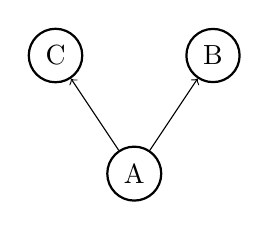
\begin{tikzpicture}[scale=0.5]
            \begin{scope}[every node/.style={circle,thick,draw}]
                \node (A) at (0,0) {A};
                \node (B) at (2,3) {B};
                \node (C) at (-2,3) {C};
            \end{scope}

            \begin{scope}
                \path [->] (A) edge node {} (B);
                \path [->] (A) edge node {} (C);
            \end{scope}
            \end{tikzpicture}
          \captionsetup{labelformat=empty}
          \caption{$\{\emptyset\}$}
        \end{subfigure}
        \begin{subfigure}{.15\textwidth}
            \centering
            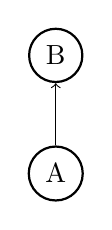
\begin{tikzpicture}[scale=0.5]
              \begin{scope}[every node/.style={circle,thick,draw}]
                  \node (A) at (0,0) {A};
                  \node (B) at (0,3) {B};
              \end{scope}

              \begin{scope}
                  \path [->] (A) edge node {} (B);
              \end{scope}
              \end{tikzpicture}
            \captionsetup{labelformat=empty}
            \caption{$\{\emptyset\}$}
          \end{subfigure}
        \begin{subfigure}{.15\textwidth}
          \centering
          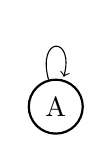
\begin{tikzpicture}[scale=0.5]
            \begin{scope}[every node/.style={circle,thick,draw}]
                \node (A) at (0,-1) {A};
            \end{scope}

            \begin{scope}
                \path [->] (A) edge [loop above] node {} (A);
            \end{scope}
            \end{tikzpicture}
          \captionsetup{labelformat=empty}
          \caption{$A = \{A\}$}
        \end{subfigure}
        \begin{subfigure}{.25\textwidth}
            \centering
            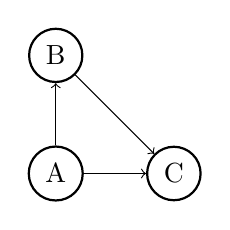
\begin{tikzpicture}[scale=0.5]
              \begin{scope}[every node/.style={circle,thick,draw}]
                  \node (A) at (0,0) {A};
                  \node (B) at (0,3) {B};
                  \node (C) at (3,0) {C};
              \end{scope}

              \begin{scope}
                  \path [->] (A) edge node {} (B);
                  \path [->] (B) edge node {} (C);
                  \path [->] (A) edge node {} (C);
              \end{scope}
              \end{tikzpicture}
            \captionsetup{labelformat=empty}
            \caption{$\{\emptyset, \{\emptyset\}\}$}
          \end{subfigure}

        \caption{Rappresentazione di insiemi tramite grafi}
        \label{fig:graph_set}
    \end{figure}
    In Figura \ref{fig:graph_set} sono rappresentati alcuni insiemi sotto forma di APG.
\end{example}

\subsection{Bisimulazione}
In questa sezione introdurremo la definizione di bisimulazione ed alcune proprietà immediate. In seguito esamineremo la relazione tra la teoria degli insiemi e la bisimulazione.
\subsubsection{Definizione e risultati generali}
\begin{definition}
    Siano $G_1 = (V_1,E_1), G_2 = (V_2,E_2)$ due grafi diretti. Una relazione binaria $R: V_1 \times V_2$ è una \emph{bisimulazione} su $G_1, G_2$ se $\forall a \in V_1, b \in V_2$ valgono congiuntamente le seguenti proprietà:
    \begin{itemize}
        \item $a R b, a E_1 a' \implies \exists b' \in V_2 : (a' R b' \land b E_2 b')$
        \item $a R b, b E_2 b' \implies \exists a' \in V_1 : (a' R b' \land a E_1 a')$
    \end{itemize}
    Analogamente si definisce una bisimulazione su un unico grafo diretto $G$, ponendo $G_1 = G_2 = G$.
\end{definition}
L'esistenza di una bisimulazione tra due grafi, come vedremo, è estremamente interessante se siamo interessati agli insiemi rappresentati dai grafi considerati:
\begin{definition}
    Siano $G_1 = (V_1,E_1), G_2 = (V_2,E_2)$ due grafi. Essi sono \emph{bisimili} se esiste una bisimulazione su $G_1, G_2$.\\
    Due APG $(G_1, v_1), (G_2, v_2)$ sono \emph{bisimili} se $G_1, G_2$ sono bisimili e vale $v_1 R v_2$ per almeno una bisimulazione $R$ su $G_1, G_2$.
\end{definition}
\begin{observation}
    Una bisimulazione può non essere riflessiva, simmetrica, nè transitiva.
\end{observation}
\begin{example}
    La relazione $a R b \iff$ ``$a,b$ sono lo stesso nodo'' su un grafo qualsiasi è una bisimulazione riflessiva, simmetrica e transitiva.\\
    La relazione $R = \emptyset$ è una bisimulazione su un grafo qualsiasi, ma non è riflessiva.\\
    La relazione $R = \{(a,a),(b,b),(c,c),(d,d),(a,b),(b,c),(c,d)\}$ sul grafo $G = (\{a,b,c,d\}, \{(a,b),(b,c),(c,d),(d,d)\})$ è una bisimulazione, ed è solamente riflessiva.
\end{example}
Dalla definizione di bisimulazione possiamo dedurre una proprietà interessante delle chiusure:
\begin{theorem}
    Sia $R$ una bisimulazione sul grafo diretto $G$. La sua chiusura riflessiva, simmetrica o transitiva è ancora una bisimulazione su $G$.
\end{theorem}
\begin{proof2}
    Consideriamo separatamente le tre relazioni $R_r, R_s, R_t$, rispettivamente la chiusura riflessiva, simmetrica e transitiva:
    \begin{itemize}
        \item $R_r$: Per definizione $R \subset R_r$, quindi è sufficiente dimostrare che $R_r$ è una bisimulazione quando gli argomenti $u,v \in V$ non sono distinti.\\
        Sia $u \in V$. Chiaramente per definizione di $R_r$ si ha $u R_r u$. Se $\exists u' \in V: u E u'$ allora (sempre per definizione di $R_r$) si ha $u' R_r u'$.
        \item $R_s$: Per definizione $R \subset R_s$, quindi è sufficiente dimostrare che $R_s$ è una bisimulazione quando per $u,v \in V$ si ha $u R v$ ma non $v R u$.\\
        Sia $(u,v) \in V\times V$. Allora:
        \begin{center}
            $u R_s v \implies u R v \lor v R u$
        \end{center}
        Supponiamo ad esempio che $v R u$.
        \begin{align*}
            &\implies \forall v' \in V: (v E v') \,\,\exists u' \in V: (u E u' \land v' R u')\\
            &\implies u' R_s v'
        \end{align*}
        e
        \begin{align*}
            &\implies \forall u' \in V: (u E u') \,\,\exists v' \in V: (v E v' \land v' R u')\\
            &\implies u' R_s v'
        \end{align*}
        cioè sono dimostrate le due condizioni caratteristiche della bisimulazione.\\
        La dimostrazione è analoga se $u R v$.
        \item $R_t$: Per definizione $b \subset R_t$, quindi è sufficiente dimostrare che $R_t$ è una bisimulazione quando per gli argomenti $u,v,z \in V$ si ha $u R v$, $v R z$ ma non $u R z$.\\
        Sia $(u,v,z) \in V\times V\times V$ con questa proprietà. Allora $\forall u' \in V: u E u' \implies \exists v' \in V: v E v' \land u' R v'$. Inoltre $\exists z' : z E z' \land v' R z'$.\\
        Riordinando si ha $u' R v', v' R z'$. Allora per definizione di $b_t, \, u' R_t z'$.\\
        In modo speculare si ottiene la seconda condizione caratteristica della bisimulazione.
    \end{itemize}
    \vspace*{-0.75cm}
\end{proof2}
Da questa proposizione si deduce il seguente corollario, che risulta dall'applicazione iterata delle tre chiusure viste in precedenza:
\begin{corollary}
    Ad ogni bisimulazione $R$ è possibile associare una bisimulazione $\widetilde{R} : R \subset \widetilde{R} \,\,\land\,\, \widetilde{R}$ è una relazione di equivalenza.
    \label{cor:bisimulation_eqrel}
\end{corollary}
Concludiamo la sezione relativa ai risultati generali sulla bisimulazione con la seguente proposizione, che sarà utile nel seguito:
\begin{proposition}
    Siano $R_1, R_2$ due bisimulazioni su $G_1, G_2$. Allora $R = R_1 \cup R_2$ è ancora una bisimulazione.
    \label{obs:bisimulation_union}
\end{proposition}
\begin{proof2}
    Siano $u,v : u R v$. Sia $u' : u E u'$. Allora deve essere $u R_1 v \lor u R_2 v$. Ma quindi $\exists v' : (v E v' \land u' R_{1|2} v')$.
\end{proof2}

\subsubsection{Bisimulazione massima}
\label{sec:bisi_max}
Definiamo ora il concetto di \emph{bisimulazione massima}, che gioca un ruolo chiave nella risoluzione dei problemi considerati in questo elaborato:
\begin{definition}
    Una bisimulazione $R_M$ su $G_1, G_2$ è \emph{massima} se per ogni bisimulazione $R$ su $G_1,G_2$ si ha $u R v \implies u R_M v$.
\end{definition}
\begin{observation}
    Sia $R_M$ la bisimulazione massima su un grafo diretto $G$. Allora per qualsiasi altra bisimulazione $R$ su $G$ si ha $|R_M| \geq |R|$.
\end{observation}
Naturalmente la bisimulazione massima dipende dai due grafi presi in esame. Possiamo dedurre alcune caratteristiche banali:
\begin{proposition}
    Valgono le seguenti proprietà:
    \begin{enumerate}
        \item La bisimulazione massima su due grafi $G_1,G_2$ è unica;
        \item La bisimulazione massima è una relazione di equivalenza.
    \end{enumerate}
    \vspace*{-0.3cm}
    \label{prop:bisi_max_equi}
\end{proposition}
\begin{proof2}
    Le proprietà seguono dal Corollario \ref{cor:bisimulation_eqrel} e dall'Osservazione \ref{obs:bisimulation_union}:
    \begin{enumerate}
        \item Supponiamo per assurdo che esistano due bisimulazioni massime $R_{M_1}, R_{M_2}$. La loro unione è ancora una bisimulazione, che è "più massima" delle supposte bisimulazioni massime.
        \item Se per assurdo la bisimulazione massima non fosse una relazione di equivalenza, potremmo considerare la sua chiusura riflessiva, simmetrica e transitiva, che avrebbe cardinalità maggiore o uguale, e sarebbe per costruzione una relazione di equivalenza.
    \end{enumerate}
    \vspace*{-0.7cm}
\end{proof2}
Naturalmente il concetto di \emph{bisimulazione massima} può essere definito anche su unico grafo diretto $G$. Questo caso si rivelerà di grande interesse nel seguito. Per ora dimostriamo il seguente risultato:
\begin{theorem}
    Sia $G$ un grafo diretto finito. Allora $\exists R_M$ la bisimulazione massima su $G$.
\end{theorem}
\begin{proof2}
    Può esistere solamente un numero finito di relazioni binarie su $G$, e questo numero fornisce un limite superiore al numero massimo di bisimulazioni su $G$.
    Allora possiamo considerare l'unione di questo numero finito di bisimulazioni, che sarà chiaramente la bisimulazione massima.
\end{proof2}

\subsubsection{Interpretazione insiemistica della bisimulazione}
Mostriamo ora una conseguenza diretta dell'Assioma di Estensionalità e di AFA:
\begin{theorem}
    Due APG rappresentano lo stesso insieme $\iff$ sono bisimili.
    \label{theo:bisi_iff_eqsets}
\end{theorem}
\begin{proof2}
    Dimostriamo separatamente le due implicazioni:
    \begin{enumerate}
        \item[$(\implies)$] Osserviamo innanzitutto che la relazione binaria $\equiv$ su $V_A, V_B$ definita come segue:
              \begin{gather*}
                  a \equiv b \iff ``\text{le decorazioni di } A,B \text{ associano ad } a,b \text{ lo stesso insieme}''
              \end{gather*}
              è una bisimulazione sui grafi $G_A = (V_A, E_A), G_B = (V_B, E_B)$.\\
              Chiaramente se $a \equiv b, a E a'$ si ha:
              \begin{itemize}
                  \item $a' \in a$, associando ad $a,a'$ gli insiemi che rappresentano secondo la decorazione (l'unica) considerata;
                  \item $a,b$ rappresentano lo stesso insieme.
              \end{itemize}
              Quindi per l'Assioma di Estensionalità $\exists b' \in b: b' = a'$, cioè $b E b'$ e $a' \equiv b'$. Si procede specularmente per la seconda condizione caratteristica della bisimulazione.\\
              La relazione $\equiv$ è una bisimulazione sugli APG $A,B$ quando si assume per ipotesi che $A,B$ rappresentino lo stesso insieme.
        \item[$(\impliedby)$] Sia $R$ una bisimulazione su $A,B$. Consideriamo la decorazione $d_A$ (l'unica) di $A$. Vogliamo estrapolarne una decorazione per $B$. Dalla possibilità di operare questo procedimento, dall'Assioma di Estensionalità e da AFA potremo dedurre l'uguaglianza degli insiemi rappresentati.\\
              Definiamo l' applicazione $d$, che ad ogni nodo di $B$ associa un insieme:
              \begin{gather*}
                  d(v) = d_A(u), \text{con $u$ nodo di $A$} : u R v
              \end{gather*}
              \begin{observation*}
                  Per ogni nodo $v$ di $B$ deve esistere almeno un nodo $u$ di $A : u R v$ perchè si suppone che i due APG siano bisimili.
              \end{observation*}
              Dimostriamo che $d$ è una decorazione di $B$. In altre parole vogliamo dimostrare che per ogni nodo $v$ di $B$ l'insieme $d(v)$ contiene tutti e soli gli
              insiemi $d(v') \,\,\forall v'$ nodo di $B : v E v'$.
              \begin{itemize}
                  \item Supponiamo per assurdo che tra i figli di $v$ ``manchi" il nodo corrispondente ad un elemento $X \in d(v)$. Poichè la decorazione di $A$ è ben definita,
                        il nodo $u$ di $A : u R v$ deve avere un figlio corrispondente a $X$, che chiameremo $u'$. Ma $u R b, u E u' \implies \exists v' : v E v', u' R v'$.
                        Cioè $d(v') = X$. Dunque il nodo mancante è stato identificato.
                  \item Supponiamo per assurdo che tra i figli di $v$ ci sia un nodo ``in più'', ovvero un nodo $v' : v E v', d(v') = Y$ con $Y \notin d(v)$. Ma
                        allora, sempre considerando $u$ il nodo di $A : u R v$, dovrebbe esistere un $u' : u E u', u' R v'$, cioè $d_A(u') = d(v') = Y$.
                        Ma allora $Y \in d_A(u) = d(v)$, deduzione che è chiaramente in contrasto con l'ipotesi.
              \end{itemize}
              E' possibile che ci siano due nodi di $a_1, a_2$ di $A$ ed un nodo $b$ di $B$ per cui vale $a_1 R b \land a_2 R b$. In questo caso la decorazione definita è ambigua.
              Per questo motivo correggiamo la formulazione di $d$ come segue:
              \begin{gather*}
                d(v) = X \text{, con $X$ l'insieme associato al nodo $u$ di $A$} : u R v, \\
                \text{con $u$ preso casualmente tra i nodi di $A$ bisimili a $v$.}
              \end{gather*}
              Per AFA esiste un'unica decorazione di $b$, quindi si deve avere, alternativamente, per ogni nodo $v$ di $B$:
              \begin{itemize}
                  \item $\exists ! u$ nodo di $A$ : $u R v$;
                  \item $\forall u$ nodo di $A$ : $u R v$, la decorazione di $A$ associa a tutti gli $u$ lo stesso insieme.
              \end{itemize}
              Dunque l'ambiguità è risolta.
    \end{enumerate}
    \vspace*{-0.75cm}
\end{proof2}
Tenendo conto di quanto affermato nella sezione \ref{sec:graphs_sets}, il Teorema \ref{theo:bisi_iff_eqsets} dimostra che la bisimulazione può sostituire la relazione di uguaglianza tra insiemi quando questi sono rappresentati con APG \cite{dovier}.\\

Dopo questa considerazone possiamo dare la seguente definizione:
\begin{definition}
    \label{def:bisi_contraction}
    Sia $R$ una bisimulazione su $G = (V,E)$, dove $G$ è un grafo diretto. Supponiamo che $R$ sia una relazione di equivalenza. Il grafo, definito a partire dal grafo iniziale, ottenuto con una \emph{contrazione rispetto alla bisimulazione} $R$, è il grafo diretto $G_R = (V_R, E_R)$ come in \cite{gentilini},  \emph{di} $G$:
    \begin{itemize}
        \item $V_R = \{[m]_R, m \in V\}$;
        \item $[m]_R E_R [n]_R \iff \exists b \in [m]_R, c \in [n]_R : b E c$.
    \end{itemize}
    Si chiama \emph{classe} del nodo $a$ rispetto alla bisimulazione $R$, indicata con la notazione $[a]_R$, il nodo di $V_R$ in cui viene inserito il nodo $a$.
\end{definition}
La Definizione \ref{def:bisi_contraction} è di fondamentale importanza per la seguente osservazione:
\begin{proposition}
    Sia $G$ un grafo diretto, e sia $G_R$ come nella Definizione \ref{def:bisi_contraction}, per una bisimulazione $R$ qualsiasi. Allora $G, G_R$ sono bisimili.
    \label{prop:bisi_cont_bisi}
\end{proposition}
\begin{proof2}
    Sia ``$\equiv$'' la relazione binaria su $V\times V_R$ definita come segue:
    \begin{gather*}
        m \equiv M \iff M = [m]_R
    \end{gather*}
    Vogliamo dimostrare che tale relazione è una bisimulazione sui grafi $G, G_R$.\\
    Supponiamo che $x \equiv X$, e che $x E y$ per qualche $y \in V$. Chiamiamo $Y \coloneqq [y]_R$. Allora, per la Definizione \ref{def:bisi_contraction}, si ha $X E_R Y$. Inoltre vale banalmente $y \equiv Y$.\\
    Per dimostrare la seconda condizione caratteristica della bisimulazione, supponiamo che $x \equiv X$, e che $X E_R Y$ per qualche $Y \in V_R$. Sempre per la Definizione \ref{def:bisi_contraction} deve esistere un $y \in Y : (y \equiv Y \land x E y)$.
\end{proof2}
La Proposizione \ref{prop:bisi_cont_bisi} ha una conseguenza ovvia, che risulta evidente dal Teorema \ref{theo:bisi_iff_eqsets}:
\begin{corollary}
    Sia $R$ una bisimulazione che sia anche una relazione di equivalenza. Allora l'APG $(G, v)$ e l'APG $(G_R, [v]_R)$ rappresentano lo stesso insieme.
\end{corollary}
Quindi risulta naturale sfruttare le proprietà della bisimulazione per minimizzare la rappresentazione di insiemi, considerando che è sufficiente una bisimulazione sulla rappresentazione iniziale per ottenere una rappresentazione equivalente. Definiamo una relazione d'ordine sulle rappresentazioni:
\begin{definition}
    Diremo che la rappresentazione $(G_a, v_a)$ di un insieme è \emph{minore} della rappresentazione equivalente $(G_b, v_b)$ se $|Va| < |Vb|$.\\
    Diremo che una rappresentazione è \emph{minima} se non esiste una rappresentazione equivalente minore.
\end{definition}
\begin{observation}
    La \emph{contrazione per bisimulazione} è una rappresentazione minore (o eventualmente uguale) di quella iniziale.
\end{observation}
Concludiamo la sezione con il seguente risultato, che stabilisce in modo univoco la bisimulazione prescelta per minimizzare la rappresentazione di un dato insieme:
\begin{theorem}
    Sia $(G,v)$ un APG rappresentante un insieme. Sia $R_M$ la bisimulazione massima su $(G,v)$. Allora la contrazione per bisimulazione indotta da $R_M$ su $(G,v)$ fornisce la rappresentazione minima dell'insieme.
\end{theorem}
\begin{proof2}
    Supponiamo per assurdo che esista una bisimulazione $R_V$ su $(G,v)$ che fornisce una contrazione avente un numero di nodi strettamente inferiore alla contrazione indotta da $R_M$. Ma questo implica che esistono almeno due nodi di $G$ che sono in relazione secondo $R_V$ e non secondo $R_M$. Chiaramente questa deduzione è in contrasto con il fatto che $R_M$ è la bisimulazione massima.\\
    Supponiamo per assurdo che, dopo la contrazione indotta da $R_M$, sia possibile trovare una nuova bisimulazione $R_O$ su $(G_{R_M}, [v]_{R_M})$ che induca una contrazione avente un numero di nodi strettamente inferiore a quello di $(G_{R_M}, [v]_{R_M})$. Chiaramente $R_O \subset V{R_M} \times V{R_M}$.\\
    Definisco una nuova bisimulazione $R_{\widetilde{M}} \subset V\times V$ tale che
    \begin{gather*}
        x R_{\widetilde{M}} y \iff (x R_M y \lor [x]_{R_M} R_O [y]_{R_M})
    \end{gather*}
    Per definizione di bisimulazione massima bisogna avere $R_{\widetilde{M}} \subset R_M$, quindi non è possibile che la contrazione indotta da $R_O$ sia una rappresentazione minore di quella indotta da $R_M$.
\end{proof2}

\subsection{Relational stable coarsest partition}
\label{sec:rscp}
In questa sezione introdurremo il concetto di \emph{RSCP} o \emph{Relational Stable Coarsest Partition}. Nel seguito del lavoro evidenzieremo il legame tra questo problema e quello della determinazione della bisimulazione massima. Questo legame viene sfruttato dagli algoritmi che tratteremo nel seguito in quanto la formulazione del primo lo rende un problema più facilmente approcciabile dal punto di vista algoritmico.\\
Cominciamo con alcune definizioni su cui struttureremo la formulazione del problema:
\begin{definition}
    Sia $S$ un insieme finito. Sia $X = \{x_1, \dots, x_n\}$ con $x_i \subseteq S \,\,\,\forall i \in \{1,\dots,n\}$. $X$ è una \emph{partizione} di $S$ se:
    \begin{gather*}
        \bigcup_{i = 1}^n x_i = A \qquad \land \qquad x_i \cap x_j = \emptyset \,\,\forall i,j \in \{1,\dots,n\} \qquad \land \qquad x_i \neq \emptyset \,\,\forall i
    \end{gather*}
    Inoltre gli insiemi $x_i$ sono i \emph{blocchi} della partizione $X$. Se $a \in x_i$ si usa la notazione $[a]_X = x_i$.
\end{definition}
\begin{observation}
    \label{obs:part_banale}
    Ogni insieme $S$ ha una partizionamento banale, consistente in un unico blocco contenente tutti gli elementi dell'insieme.
\end{observation}
\begin{example}
    TROVA ESEMPIO
    \label{exa:set_partition}
\end{example}
\begin{definition}
    Siano $X_1,X_2$ due partizioni dello stesso insieme. $X_2$ \emph{rifinisce} $X_1$ se $\forall x_2 \in X_2, \,\,\exists x_1 \in X_1 : x_2 \subseteq x_1$.
\end{definition}
\begin{example}
    TROVA ESEMPIO
\end{example}
Il partizionamento di insiemi finiti assume interesse nell'ambito trattato in questo lavoro quando si impone la seguente condizione sui blocchi:
\begin{definition}
    Sia $S$ un insieme, ed $R$ una relazione binaria su $S$. Sia $X$ una partizione su $S$, e sia $B \subseteq A$.
    \begin{itemize}
        \item $X$ è stabile rispetto alla coppia $(B,R)$ se $\forall x \in X$ vale $x \subseteq R^{-1}(B) \lor x_i \cap R^{-1}(B) = \emptyset$;
        \item La partizione $X$ è \emph{stabile} rispetto ad $R$ se è stabile rispetto a $(x,R) \,\,\forall x \in X$.
    \end{itemize}
\end{definition}
\begin{example}
    \label{exa:set_partition_stable}
    TROVA ESEMPIO
\end{example}
In altre parole per ogni coppia di blocchi di una partizione stabile si hanno due alternative:
\begin{itemize}
    \item Tutti gli elementi del primo blocco sono in relazione con almeno un elemento del secondo blocco;
    \item Nessuno degli elementi del primo blocco è in relazione con qualche elemento del secondo blocco.
\end{itemize}
Vale la seguente osservazione banale:
\begin{observation}
    Sia $X$ una partizione qualsiasi di un insieme $U$, e siano $S,T \subseteq U$. Sia $R$ una relazione binaria su $U$. Supponiamo $X$ stabile rispetto alle coppie $(R,S),(R,T)$. Allora:
    \begin{enumerate}
        \item Qualsiasi rifinitura di $P$ resta stabile rispetto alla coppia $(f,S)$;
        \item $P$ è stabile rispetto alla coppia $(f,S \cup T)$.
    \end{enumerate}
\end{observation}
\begin{proof2}
    Dimostriamo separatamente i due enunciati:
    \begin{enumerate}
        \item Chiaramente se per un blocco qualsiasi $x \in X$ vale $x \subseteq R^{-1}(S) \lor x \cap R^{-1}(S) = \emptyset$, la stessa relazione vale per qualsiasi sottoinsieme di $x$;
        \item Sia $x \in X$. Chiaramente vale $R^{-1}(S),R^{-1}(T) \subseteq R^{-1}(S \cup T)$. Allora, se almeno uno tra $R^{-1}(S),R^{-1}(T)$ contiene l'immagine di $x$ si avrà $x \subseteq R^{-1}(S \cup T)$, altrimenti $x \cap R^{-1}(S \cup T)$ dovrà chiaramente essere vuoto.
    \end{enumerate}
    \vspace*{-0.75cm}
\end{proof2}

Con queste premesse possiamo definire il problema della determinazione della RSCP:
\begin{definition}
    Sia $A$ un insieme, sia $R$ una relazione binaria su $A$. Sia $S$ una partizione di $A$. la ``RSCP($S,R$)'' di $A$ è la partizione di $A$ stabile rispetto ad $R$, che rifinisce $S$ e che contiene il minor numero di blocchi (per questo motivo si dice che è la \emph{più rozza}).\\
    Si usa la notazione ``RSCP$(R)$'' se la partizione iniziale è quella banale proposta nella Definizione \ref{obs:part_banale}.
\end{definition}
\begin{example}
    TROVA ESEMPIO
\end{example}
La seguente definizione ha grande importanza pratica per il problema della determinazione della RSCP:
\begin{definition}
    \label{def:funz_split}
    Sia $\widetilde{S} = \{S_1,\dots,S_n\}$ una partizione qualsiasi di un insieme finito $S$. Sia $f: S E S$, e sia $A \subset S$. $A$ è uno \emph{splitter} di $S$ rispetto a $f$ se
    \begin{gather*}
        \exists S_x \in \widetilde{S} : \qquad S_x \cap f^{-1}(A) \neq \emptyset \,\,\land\,\, S_x \not\subseteq f^{-1}(A)
    \end{gather*}
    ovvero se la partizione non è stabile rispetto ad $A$. In tal caso definiamo la seguente funzione:
    \begin{gather*}
        \text{Split}(A,\widetilde{S}) = \{S_x \cap f^{-1}(A), S_x - f^{-1}(A) \quad \forall S_x \in \widetilde{S}\} - \{\emptyset\}
    \end{gather*}
\end{definition}
Valgono le seguenti osservazioni sulla funzione appena introdotta:
\begin{observation}
    Se $A$ non è uno \emph{splitter} di $\widetilde{S}$ si ha $\widetilde{S} = $ Split$(A,\widetilde{S})$.
\end{observation}
\begin{observation}
    \label{obs:split_eredita}
    Se $\widetilde{S}$ è stabile rispetto ad un insieme $A$, Split$(B,\widetilde{S})$ è stabile rispetto ad $A,B$. In altre parole la funzione ``Split'' preserva la stabilità.
\end{observation}
\begin{proof2}
    Osservando che ``Split'' può solamente dividere i blocchi, e non mescolarli, la dimostrazione è banale.
\end{proof2}
Dimostriamo il seguente risultato che useremo nel seguito:
\begin{theorem}
    \label{theo:split_properties}
    Consideriamo la funzione ``Split'' proposta nella Definizione \ref{def:funz_split}:
    \begin{enumerate}
        \item La funzione è monotona rispetto al secondo argomento, cioè se $\widetilde{S}$ è una rifinitura di $S$, allora Split$(A,\widetilde{S})$ rifinisce Split$(A,S)$;
        \item La funzione è commutativa rispetto al primo argomento: Split$(A,$ Split$(B,S)) =$ Split$(B,$ Split$(A,S))$.
    \end{enumerate}
\end{theorem}
\begin{proof2}
    Dimostriamo separatamente gli enunciati:
    \begin{enumerate}
        \item I blocchi di Split$(A,\widetilde{S})$ sono del tipo $x - R^{-1}(A)$ oppure $x \cap R^{-1}(A)$, dove $x$ è un blocco di $\widetilde{S}$. I blocchi di Split$(A,S)$ sono del tipo $y - R^{-1}(A)$ oppure $y \cap R^{-1}(A)$, dove $y$ è un blocco di $S$. Poichè $\forall x \in \widetilde{S} \,\,\exists y \in S : x \subseteq y$ si ha $x - R^{-1}(A) \subseteq y - R^{-1}(A)$ e $x \cap R^{-1}(A) \subseteq y \cap R^{-1}(A)$;
        \item Conseguenza della commutatività delle operazioni ``$-$'' e ``$\cap$'' su insiemi.
    \end{enumerate}
    \vspace*{-0.75cm}
\end{proof2}

\subsection{Equivalenza tra RSCP e bisimulazione massima}
Dimostriamo innanzitutto il seguente risultato preliminare presentato in \cite{gentilini}:
\begin{proposition}
    Sia $G = (V,E)$. Sia $X$ una partizione di $V$ stabile rispetto a $E$. Allora la relazione binaria $R$ su $V$ definita come:
    \begin{gather*}
        a R b \iff [a]_X = [b]_X
    \end{gather*}
    è una bisimulazione su $G$.
    \label{prop:part_induce_bisi}
\end{proposition}
\begin{proof2}
    Siano $a,b \in G : a R b$, e sia $a' : a E a'$. Poichè $X$ è stabile, si ha che $[a]_X \subseteq E^{-1}([a']_X)$. Quindi $\exists b' \in [a']_X : b E b'$.\\
    L'altra condizione caratteristica della bisimulazione si dimostra in modo speculare.
\end{proof2}
In altre parole, una qualsiasi partizione stabile rispetto a $E$ induce su un grafo diretto una bisimulazione che può essere ricavata in modo banale.\\
Dimostriamo ora il risultato opposto:
\begin{proposition}
    Sia $R$ una bisimulazione su $G$ che sia anche una relazione di equivalenza. Allora la partizione i cui blocchi sono le classi di equivalenza di $R$ è stabile rispetto a $E$.
    \label{prop:bisi_induce_part}
\end{proposition}
\begin{proof2}
    Se per assurdo $X$ non fosse stabile esisterebbero due blocchi $x_1, x_2 : x_1 \,\,\cap E^{-1}(x_2)$ non è ne $x_1$ nè $\emptyset$. Chiamiamo $A$ questo insieme.\\
    Gli elementi $a$ di $A$ sono i nodi in $x_1 : \nexists b \in x_2 : a E b$. Ma poichè questi $a$ e gli $x \in x_1 - A$ si trovano all'interno dello stesso blocco $x_1$ deve valere $x R a$.\\
    Sia $x \in x_1 - A$, ed $y \in x_2 : x E y$. Poichè $\forall a \in A$ vale $x R a$, allora $\exists a' : a E a', a' R y$, cioè $[a']_X = [y]_X = x_2$. Quindi $A$ deve necessariamente essere vuoto.
\end{proof2}
Cioè una bisimulazione induce un partizionamento stabile rispetto a $E$ dei nodi del grafo. Vale il seguente corollario:
\begin{corollary}
    Determinare la bisimulazione massima su un grafo diretto $G = (V,E)$ e trovare RSCP($E$) di $V$ sono problemi equivalenti.
\end{corollary}
\begin{proof2}
    Dimostriamo separatamente che la bisimulazione ricavata dalla RSCP($E$) è massima, e che la partizione ricavata dalla bisimulazione massima è la RSCP($E$).
    \begin{itemize}
        \item Sia $R_M$ la bisimulazione massima su $G$. Per la Proposizione \ref{prop:bisi_max_equi} è una relazione di equivalenza. Per la Proposizione \ref{prop:bisi_induce_part} è possibile determinare una partizione $X$ stabile rispetto a $E$.\\
              Supponiamo per assurdo che $X$ non sia RSCP($E$) di $V$, quindi esiste una partizione $\widetilde{X}$ stabile rispetto a $E$ che ha meno blocchi di quanti ne ha $X$. Ma per la Proposizione \ref{prop:part_induce_bisi} da
              $\widetilde{X}$ è possibile ricavare una bisimulazione $\widetilde{R}$ su $G$. Ma quindi $|\widetilde{R}| > |R|$, che è assurdo.
        \item Sia $X$ la RSCP($E$) di V. Supponiamo per assurdo che la bisimulazione $R$ ricavata da $X$ come nella Proposizione \ref{prop:part_induce_bisi} non sia massima. Allora deve esistere un'altra bisimulazione $\widetilde{R}$ che
              sia massima. Ma da questa si può ricavare, come nella Proposizione \ref{prop:bisi_induce_part}, una partizione $\widetilde{X}$ stabile rispetto a $E$ per cui vale $|\widetilde{X}| \leq |X|$. Ma questo è assurdo.
    \end{itemize}
    \vspace*{-0.75cm}
\end{proof2}

\clearpage
\section{Algoritmi risolutivi}
\label{sec:algs}
In questa sezione esamineremo alcuni algoritmi risolutivi proposti per la risoluzione del problema della determinazione della massima bisimulazione su un grafo. Come risulterà evidente nel seguito viene sfruttata ampiamente l'equivalenza tra bisimulazione massima e RCSP dimostrata nella sezione precedente.

\subsection{Algoritmo di Hopcroft}
Esaminiamo innanzitutto un algoritmo risolutivo per una versione semplificata del problema, ovvero la minimizzazione di un'automa a stati finiti \cite{hopcroft}. La risoluzione di questo caso particolare ha fornito diversi spunti importanti per l'ideazione di algoritmi risolutivi più generali che saranno presentati nel seguito.

\newcommand{\automata}{$\mathcal{A} = (\mathcal{S},\mathcal{I},\mathcal{U},\mathcal{F},\delta)$ }
\newcommand{\argsautomata}{$\mathcal{S},\mathcal{I},\mathcal{U},\mathcal{F},\delta$ }

\subsubsection{Nozioni fondamentali}
Innanzitutto definiamo il concetto di \emph{automa}, chiaramente centrale nella descrizione del problema:
\begin{definition}
    Consideriamo i seguenti oggetti matematici:
    \begin{itemize}
        \item Un insieme finito $\mathcal{I}$ detto \emph{insieme degli ingressi};
        \item Un insieme finito $\mathcal{U}$ detto \emph{insieme delle uscite};
        \item Un insieme finito $\mathcal{S}$ detto \emph{insieme degli stati}, ad ogni stato è associata un'unica uscita appartenente ad $U$;
        \item Un insieme $\mathcal{F} \subseteq \mathcal{S}$ detto \emph{insieme degli stati finali};
        \item Una funzione $\delta: \mathcal{S} \times \mathcal{I} \to \mathcal{S}$ detta \emph{funzione di trasferimento}.
    \end{itemize}
    Chiameremo $A = (\mathcal{S},\mathcal{I},\mathcal{U},\delta,\mathcal{F})$ \emph{automa}. Useremo la notazione $Out(x)$ per indicare l'output corrispondente allo stato $x$.
\end{definition}
Possiamo rappresentare un'automa con una tabella degli stati, in cui ad ogni riga corrisponde uno stato, a ogni colonna un ingresso, e ogni cella contiene il nuovo stato quando, nel momento in cui il sistema si trova nello stato corrispondente alla riga, si inserisce l'ingresso corrispondente alla colonna. In alternativa possiamo utilizzare una rappresentazione grafica, in cui ogni stato è descritto da un cerchio contenente il nome dello stato, e le transizioni tra stati sono rappresentate da frecce sulle quali viene specificato l'ingresso che ha innescato la transizione.

\begin{example}
    Nella Tabella \ref{fig:tab_automata} è rappresentato un'automa che cambia stato solamente se l'ingresso è ``1'', e lo stato non è ``$c$''.
    \begin{table}[t]
        \centering
        \begin{tabular}{ c | c c }
            \hline
            & 0 & 1\\
            \hline
            a[0] & a & b \\
            b[0] & b & c \\
            c[1] & c & c \\
            \hline
          \end{tabular}
        \caption{Rappresentazione tabellare di un'automa.}
        \label{fig:tab_automata}
    \end{table}
    \label{exa:automata_tab}
\end{example}

\begin{example}
    Nella Figura \ref{fig:automata} è rappresentato lo stesso automa dell'Esempio \ref{exa:automata_tab}.
    \begin{figure}[t]
        \centering
        \begin{tikzpicture}[->,>=stealth',shorten >=1pt,auto,node distance=3.5cm,
            scale = 1,transform shape]
            \node[state] (a) {$a[0]$};
            \node[state] (b) [right of=a] {$b[0]$};
            \node[state] (c) [right of=b] {$c[1]$};

            \path (a) edge              node {$1$} (b)
                  (b) edge              node {$1$} (c)
                  (a) edge [loop above]             node {$0$} (a)
                  (b) edge [loop above]             node {$0$} (b)
                  (c) edge [loop above]              node {$0/1$} (c);
        \end{tikzpicture}
        \caption{Rappresentazione grafica di un'automa.}
        \label{fig:automata}
    \end{figure}
\end{example}

In alcuni automi è possibile individuare stati che ``si comportano in modo simile''. Informalmente possiamo dire che due stati $a,b \in \mathcal{S}$ tali che $Out(a) = Out(b)$ si comportano in modo simile quando i due stati in cui ricade il sistema in seguito ad una transizione innescata da uno stesso input $i$ a partire dagli stati $a$ o $b$ (ovvero i due stati $\delta(a,i), \delta(b,i)$) si comportano in modo simile. In Figura \ref{fig:automata_eq} illustriamo un esempio di questa situazione: consideriamo gli stati dell'automa rappresentato. Supponiamo di accorpare gli stati $b,c$ in un unico stato, che chiamiamo $B'$. Se ci interessiamo solamente alla sequenza di output ed all'eventuale raggiungimento di uno stato finale, il nuovo automa risulta indistinguibile dal primo.

\begin{example}
    \begin{figure}[b]
        \centering
        \begin{tikzpicture}[->,>=stealth',shorten >=1pt,auto,node distance=3.5cm,
            scale = 1,transform shape]
            \node[state] (a) {$A[0]$};
            \node[state] (b) [right of=a] {$B[1]$};
            \node[state] (c) [right of=b] {$C[1]$};

            \path (a) edge              node {$1$} (b)
                  (b) edge [bend right]             node {$1$} (c)
                  (c) edge [bend right]             node {$1$} (b)
                  (a) edge [loop above]             node {$0$} (a)
                  (b) edge [loop above]             node {$0$} (b)
                  (c) edge [loop above]             node {$0$} (c);
        \end{tikzpicture}
        \caption{Automa contenente stati equivalenti.}
        \label{fig:automata_eq}
    \end{figure}
    In questo esempio gli stati $B,C$ sono equivalenti secondo la definizione informale proposta sopra.
\end{example}

Proponiamo una possibile definizione formale di equivalenza tra stati. Nel seguito ne dedurremo una equivalente, che consente di stabilire un parallelo con gli argomenti trattati nella Sezione \ref{sec:base}.
\begin{definition}
    \label{def:equivalent_states}
    Sia $\mathcal{I}^*$ l'insieme di tutte le sequenze di input di lunghezza finita. Sia $\delta^* : \mathcal{S} \times \mathcal{I}^*$ la funzione di transizione ``iterata''. Due stati $x,y \in \mathcal{S}$ sono equivalenti se e soltanto se valgono congiuntamente le seguenti condizioni:
    \begin{enumerate}
        \item $Out(x) = Out(y)$;
        \item $\forall i^* \in \mathcal{I}^*,\,\, \delta^*(x,i^*) \in \mathcal{F} \iff \delta^*(y,i^*) \in \mathcal{F}$.
    \end{enumerate}
    Se le condizioni valgono utilizzermo la notazione ``$x \sim y$''.
\end{definition}

\begin{observation}
    La relazione ``$\sim$'' è una relazione di equivalenza sull'insieme degli stati di un'automa.
\end{observation}

La seguente proposizione sarà utile per formulare il problema con la terminologia esposta nella Sezione \ref{sec:rscp}:
\begin{proposition}
    \label{prop:equivalent_states}
    Due stati $x,y$ sono equivalenti nel senso della definizione \ref{def:equivalent_states} se e solo se
    \begin{gather}\label{hop:alternative_sim}
        \forall i \in \mathcal{I}, \quad \delta(x,i) \sim \delta(y,i)
    \end{gather}
    e $Out(x) = Out(y)$.
\end{proposition}
\begin{proof2}
    Supponiamo che $\exists i \in \mathcal{I} : \delta(x,i) \not\sim \delta(y,i)$. Allora, ad esempio:
    \begin{gather*}
        \exists i^* \in \mathcal{I}^* : \delta^*(\delta(x,i),i^*) = \delta^*(x,ii^*) \in \mathcal{F}, \,\, \delta^*(\delta(y,i),i^*) = \delta^*(y,ii^*) \notin \mathcal{F}
    \end{gather*}
    Quindi, per l'esistenza della stringa $ii^*$ si ha $x \not\sim y$. La dimostrazione è speculare se $\exists i^* \in \mathcal{I}^* : \delta^*(x,ii^*) \notin \mathcal{F}, \delta^*(y,ii^*) \in \mathcal{F}$.

    Ora supponiamo che valga la \ref{hop:alternative_sim}. \accente chiaro che $\forall i^* \in \mathcal{I}^*$ si ha:
    \begin{gather*}
        \delta^*(x,ii^*) \sim \delta^*(y,ii^*) \forall i \in \mathcal{I}
    \end{gather*}
    e quindi $x \sim y$.
\end{proof2}

\begin{proposition}
    La relazione ``$\sim$'' è una bisimulazione sull'insieme $\mathcal{S}$, con la relazione binaria $\displaystyle E \,\,\coloneqq \bigcup_{i \in \mathcal{I}, x \in \mathcal{S}} \{(x,\delta(x,i))\}$.
\end{proposition}
\begin{proof2}
    Supponiamo che $x \sim y$. Sia $\langle x, x'\rangle \in E$, cioè $\exists i \in \mathcal{I} : x' = \delta(x,i)$. Sia $y' = \delta(y,i) \implies \langle y, y'\rangle$. Allora, per la Proposizione \ref{prop:equivalent_states}, $x' \sim y'$. Lo stesso argomento vale in modo speculare.
\end{proof2}

Osserviamo che nella definizione di $E$ si perde un'informazione importante, cioè il fatto che per $i \in \mathcal{I}$ fissato $\delta_i(x) \coloneqq \delta(x,i)$ è una funzione, ovvero l'insieme immagine di ogni $x \in \mathcal{S}$ ha cardinalità 1. L'algoritmo di Hopcroft sfrutta questa ipotesi nel procedimento che consente di migliorare l'algoritmo banale che verrà discusso nel seguito del lavoro.

Possiamo ora definire la \emph{minimizzazione per stati equivalenti} di un'automa a stati finiti:
\begin{definition}\label{def:minim_eq_states}
    Sia \automata un'automa a stati finiti. Chiameremo \emph{minimizzazione per stati equivalenti} l'automa $(\mathfrak{S}, \mathcal{I}, \mathcal{U}, \delta_\mathfrak{S}, \mathcal{F}_\mathfrak{S})$ dove
    \begin{itemize}
        \item $\mathfrak{S} = \mathcal{S} / \sim$;
        \item $\delta_\mathfrak{S} : (\mathfrak{S} \times \mathcal{I}) \to \mathfrak{S} \mid \delta(i, x) = y \implies \delta_\mathfrak{S}(i,[x]_\mathfrak{S}) = [y]_\mathfrak{S}$;
        \item $\mathcal{F}_\mathfrak{S} = \mathcal{F} / \sim$.
    \end{itemize}
\end{definition}
Si rammenta che con la notazione $A / \mathcal{R}$ ci riferiamo all'insieme delle classi di equivalenza indotte da una relazione di equivalenza $\mathcal{R} : A \times A$ su un insieme $A$, e che con la notazione $[a]_\mathfrak{X}$ ci riferiamo al blocco di una partizione $\mathfrak{X}$ in cui viene posto $a$.

Prima di concludere l'esposizione delle nozioni preliminari è necessario dimostrare un risultato interessante che lega il problema della minimizzazzione di un'automa a stati finiti con quanto è stato presentato nella sezione \ref{sec:rscp}. A questo scopo dimostriamo i seguenti lemmi, che consentono di dimostrare tale legame in modo agevole:
\begin{lemma}
    \label{lem:part_stab_stesso_blocco}
    Sia \automata un'automa a stati finiti. Sia $\mathfrak{S}$ una partizione di $\mathcal{S}$ stabile rispetto alla famiglia di funzioni $\delta_i, i \in \mathcal{I}$. Allora $\forall (x,y) \in \mathcal{S} \times \mathcal{S}$ tali che $[x]_{\mathfrak{S}} = [y]_{\mathfrak{S}}$ si ha che $\forall i^* \in \mathcal{I}^*$:
    \begin{gather*}
        [\delta^*(x,i^*)]_{\mathfrak{S}} = [\delta^*(y,i^*)]_{\mathfrak{S}}
    \end{gather*}
\end{lemma}
\begin{proof2}
    Procediamo per induzione su $i^*$. Inizialmente i due stati si trovano nello stesso blocco di $\mathfrak{S}$. Ora supponiamo che dopo l'inserimento dell' $(n-1)$-esimo simbolo di $i^*$ i due stati $x_{n-1}, y_{n-1}$ in cui si trova l'automa appartengano ancora allo stesso blocco. La partizione è stabile rispetto alla funzione $\delta_i$, dove $i$ è l' $n$-esimo simbolo di $i^*$, quindi tutto il blocco $[x_{n-1}]_{\mathfrak{S}} = [y_{n-1}]_{\mathfrak{S}}\,\,$ è contenuto all'interno dell'insieme $\delta_i^{-1}([\delta_i(x_{n-1})]_{\mathfrak{S}}) = \delta_i^{-1}([x_n]_{\mathfrak{S}})$. Quindi $\delta_i(y_{n-1}) \in \delta_i^{-1}([x_n]_{\mathfrak{S}})$, e dunque e si ha anche $[x_n]_{\widehat{S}} = [y_n]_{\mathfrak{S}}$.
\end{proof2}

\begin{lemma}
    \label{lem:part_stab_equiv}
    Sia \automata un'automa a stati finiti. Sia $\mathfrak{S}$ una partizione di $\mathcal{S}$ stabile rispetto alla famiglia di funzioni $\delta_i, i \in \mathcal{I}$. Supponiamo inoltre che per $\mathfrak{S}$ valga la segente condizione:
    \begin{gather*}
        \forall (x,F) \in \mathcal{S} \times \mathcal{F}, \quad [x]_{\mathfrak{S}} = [F]_{\mathfrak{S}} \implies x \in \mathcal{F}
    \end{gather*}
    Allora $\forall \mathfrak{p} \in \mathfrak{S}, \,\,\forall (x,y) \in \mathfrak{p} \times \mathfrak{p}$ si ha $x \sim y$.
\end{lemma}
\begin{proof2}
    Supponiamo per assurdo che in un blocco di $\mathfrak{S}$ esistano due stati $x,y$ non equivalenti. Allora deve esistere una stringa $i^* \in \mathcal{I}^*$ tale che, ad esempio, $\delta^*(x,i^*) \in \mathcal{F} \land \delta^*(y,i^*) \not\in \mathcal{F}$. Ma per il Lemma \ref{lem:part_stab_stesso_blocco} $[\delta^*(x,i^*)]_{\mathfrak{S}} = [\delta^*(y,i^*)]_{\mathfrak{S}}$. Chiaramente questo è assurdo per la condizione assunta nell'ipotesi, quindi non possono esistere nello stesso blocco due stati non equivalenti.
\end{proof2}
A questo punto abbiamo gli ingredienti necessari per dimostrare un risultato interessante su una tipologia particolare di automi così definita:
\begin{definition}
    \label{def:automi_ben_posti}
    Un'automa a stati finiti \automata è \emph{ben posto} se $x \in \mathcal{F}, y \not\in \mathcal{F} \implies Out(x) \neq Out(y)$, ovvero l'output assegnato a stati finali è sempre diverso dall'output corrispondente a stati non finali.
\end{definition}
\begin{theorem}
    \label{theo:auto_mini_rscp}
    Sia \automata un'automa a stati finiti. La minimizzazione per stati equivalenti $(\mathfrak{S}, \mathcal{I}, \mathcal{U}, \delta_\mathfrak{S}, \mathcal{F}_\mathfrak{S})$ (Definizione \ref{def:minim_eq_states}) è l'automa avente per stati i blocchi della partizione più grossolana stabile rispetto alla famiglia di funzioni $\delta_i, i \in \mathcal{I}$.
\end{theorem}
\begin{proof2}
    Dimostriamo che $\mathfrak{S}$ è una partizione di $\mathcal{S}$ stabile rispetto alle funzioni $\delta_i$. Supponiamo per assurdo che $\exists i \in \mathcal{I} \mid \mathfrak{S}$ non è stabile rispetto a $\delta_i$. Quindi esistono $\mathfrak{s}_1, \mathfrak{s}_2 \in \mathfrak{S}$ tali che:
    \begin{gather*}
        \mathfrak{s}_1 \not\subseteq \delta_i^{-1}(\mathfrak{s}_2) \,\, \land \,\, \mathfrak{s}_1 \,\cap \,\delta_i^{-1}(\mathfrak{s}_2) \neq \emptyset
    \end{gather*}
    La prima porzione dell'espressione implica che $\exists x \in \mathfrak{s}_1 : \delta_i(x) \not\in \mathfrak{s}_2$. Ma questo è chiaramente in contrasto con l'Osservazione \ref{prop:equivalent_states}, perchè $\forall (y,Z) \in \mathfrak{s}_1 \times \mathfrak{s}_1$ deve valere $\delta_i(y) \sim \delta_i(Z)$, mentre è evidente che, poichè $\mathfrak{s}_1 \,\cap\, \delta_i^{-1}(\mathfrak{s}_2) \neq \emptyset$, c'è almeno una coppia che non soddisfa questa condizione.

    Ora supponiamo che la partizione $\mathfrak{S}$ non sia la più grossolana stabile rispetto a tutte le funzioni $\delta_i : i \in \mathcal{I}$. Ne deve esistere quindi una stabile più grossolana, che chiamiamo $\mathfrak{S}_2$. Chiaramente si ha $|\mathfrak{S}_2| < |\mathfrak{S}|$, e quindi devono esistere almeno due blocchi $\mathfrak{s}_1, \mathfrak{s}_2 \in \mathfrak{S}$ ed un blocco $\mathfrak{s}_3 \in \mathfrak{S}_2$ tali che
    \begin{gather*}
        \mathfrak{s}_1 \cap \mathfrak{s}_3 \neq \emptyset \,\,\land\,\, \mathfrak{s}_2 \cap \mathfrak{s}_3 \neq \emptyset
    \end{gather*}
    Ma questo è chiaramente in contrasto con il Lemma \ref{lem:part_stab_equiv} per come è stata costruita la partizione $\mathfrak{S}$, in quanto non possono esistere coppie di stati nello stesso blocco di $\mathcal{S}_2$ ma in un blocco diverso di $\mathcal{S}$, in quanto da quest'ultima condizione segue che $x \not\sim y$.
\end{proof2}
Osserviamo che la condizione richiesta nell'ipotesi del Teorema \ref{theo:auto_mini_rscp}, che impone l'assegnazione di un output diverso a stati finali e non finali, è estremamente debole: dato un'automa qualsiasi è sempre possibile costruirne un altro che soddisfa tale condizione, in tempo lineare rispetto al numero di stati.

\subsubsection{L'algoritmo di Hopcroft}
Il problema della minimizzazione di automi a stati finiti è stato risolto da John Hopcroft nel 1971, che ha proposto un algoritmo efficiente sfruttando un'osservazione che sarà discussa nel seguito. Presenteremo innanzitutto un algoritmo immediato, che sarà utile per un primo approccio al lato algoritmico del problema; dopodichè esamineremo lo pseudocodice dell'algoritmo di Hopcroft, e commenteremo l'intuizione che ha consentito di migliorare l'algoritmo immediato.

\paragraph{Un primo algoritmo triviale} Utilizzando i risultati della sezione precedente possiamo progettare il seguente algoritmo, il cui funzionamento è sostanzialmente lineare: per ogni ingresso $i \in \mathcal{I}$ si rifinisce la partizione iniziale (data dagli output assegnati ai vari stati) finchè non diventa stabile rispetto a $\delta_i$; dopodichè si procede con l'ingresso seguente.

\begin{algorithm}[t]
    \caption{Algoritmo triviale per la minimizzazzione di automi a stati finiti.}
    \label{alg:hop_banale}
    \SetAlgoLined
    \KwData{\argsautomata}
    \tcp*[h]{Partizione iniziale contenente un unico blocco}
    \nl$\widetilde{S} \coloneqq \{\{s_1, \dots, s_n\}\}$\;
    \tcc*[h]{Separiamo gli stati non equivalenti in base all'output}\\
    $\mathfrak{S} = \{\mathfrak{s}_k \in \mathcal{P}(\mathcal{S}) \mid Out(x) = k, \forall x \in \mathfrak{s}_k\}$\;\label{alg:hop_banale_partiziona_output}
    \ForEach{$i \in I$} {
        \label{alg:hop_banale_for_ingressi}
        \While{($\mathfrak{s}_1, \mathfrak{s}_2 =$ BlocchiNonStabili($\mathfrak{S}, \delta_i)) \neq$ None}{
            \label{alg:hop_banale_for_ns}
            \tcc*[h]{Estraiamo una coppia di blocchi che trasgredisce la condizione di stabilità.}\\
            $\widetilde{\mathfrak{s}}_1 \coloneqq \mathfrak{s}_1 - \delta_i^{-1}(\mathfrak{s}_2)$\;
            $\widehat{\mathfrak{s}}_1 \coloneqq \mathfrak{s}_1 \cap \delta_i^{-1}(\mathfrak{s}_2)$\;
            \tcp*[h]{Aggiorniamo $S$}\\
            $\mathfrak{S} = (\mathfrak{S} - \{\mathfrak{s}_1\}) \cup \{\widetilde{\mathfrak{s}}_1,\widehat{\mathfrak{s}}_1\}$\;
        }
    }
    \Return{$S$}
\end{algorithm}
La funzione ``BlocchiNonStabili'' restituisce una coppia $\mathfrak{s}_1, \mathfrak{s}_2$ di blocchi di $\mathfrak{S}$ che trasgredisce la condizione di stabilità rispetto alla funzione $\delta_i$, o ``None'' quando una tale coppia non esiste. L'algoritmo termina, perchè la condizione del ciclo diventa sicuramente falsa quando la partizione $\mathfrak{S}$ è composta da $n$ blocchi, uno per ogni stato, ed ad ogni iterazione un blocco viene diviso in due blocchi distinti e non vuoti.

Inoltre la risposta fornita è corretta, perchè l'algoritmo si ferma appena viene trovata una partizione stabile. Poichè ad ogni iterazione del ciclo definito nella Riga \ref{alg:hop_banale_for_ns} il numero di blocchi aumenta di 1, il risultato è la partizione stabile più grossolana rispetto alle funzioni $\delta_i$. Osserviamo inoltre che, se la partizione è stabile rispetto a $\delta_i$ dopo una certa iterazione del ciclo definito nella Riga \ref{alg:hop_banale_for_ingressi}, allora resta stabile fino alla fine dell'esecuzione per la Proposizione \ref{prop:rifi_stabile}.

Verifichiamo la complessità dell'algoritmo:
\begin{itemize}
    \item La Riga \ref{alg:hop_banale_partiziona_output} ha complessità $\Theta(|S|)$;
    \item Il ciclo alla Riga \ref{alg:hop_banale_for_ingressi} viene eseguito $\Theta(|I|)$ volte;
    \item La funzione ``BlocchiNonStabili'' ha complessità $O(|S|^2)$;
    \item Il ciclo alla Riga \ref{alg:hop_banale_for_ns} viene eseguito $O(|S|)$ volte;
    \item Il contenuto del ciclo alla Riga \ref{alg:hop_banale_for_ns} ha complessità $O(|S|)$ (con gli opportuni accorgimenti).
\end{itemize}
Quindi la complessità dell'algoritmo è \begin{gather*}
    T(|S|,|I|) = \Theta|I|\left[O(|S|^2 + O(|S|) * O(|S|))\right] = \Theta(I)O(|S|^2)
\end{gather*}
Se consideriamo costante il numero di ingressi: $T(|S|) = O(|S|^2)$. Seppur di facile comprensione, l'algoritmo triviale è poco efficiente a causa dei numerosi controlli per la stabilità.

\paragraph{Algoritmo di Hopcroft} Presentiamo un algoritmo che migliora la procedura triviale presentata nella sezione precedente, portando la complessità relativa alla risoluzione del problema della minimizzazione di automi a stati finiti a \emph{loglineare} \cite{hopcroft}. Forniremo un commento allo pseudocodice, in modo da spiegare il procedimento in modo dettagliato. In seguito analizzeremo formalmente l'algoritmo, proporremo e commenteremo la dimostrazione della correttezza e della complessità.\\
\afterpage{
    \begin{algorithm}[H]
        \thispagestyle{empty}
        \caption{Algoritmo di Hopcroft}
        \label{alg:hop}
        \KwData{\argsautomata}
        \Begin{
            \ForEach{$(s,i) \in \mathcal{S} \times \mathcal{I}$}{
                $\delta^{-1}(s,i) \coloneqq \{t : \delta(t,i) = s\}$\;\label{alg:hop_deltainverso}
            }
            $B(1) \coloneqq \mathcal{F}, B(2) \coloneqq \mathcal{S} - \mathcal{F}$\;
            \ForEach{$j \in \{1,2\}$}{
                \tcc*[h]{$\forall i \in \mathcal{I}$ costruiamo l'insieme degli stati in $B(j)$ aventi controimmagine non vuota rispetto  a $\delta_i$}.\\
                \ForEach{$i \in \mathcal{I}$}{
                    $i(j) = \{s : s \in B(j) \land \delta^{-1}(s,i) \neq \emptyset\}$\;\label{alg:hop_stati_delta_nonvuoto}
                }
            }
            \tcc*[h]{$k$ è il numero di blocchi della partizione, aumenta in seguito alle rifiniture.}\\
            $k \coloneqq 2$\;
            \tcc*[h]{Per ogni ingresso $i$ creiamo un insieme $L(i)$ contenente l'indice $j$ che minimizza $|i(j)|$.}\\
            \ForEach{$i \in \mathcal{I}$}{
                \label{alg:hop_splitters}
                \eIf{$|i(1)| \leq |i(2)|$}{
                    $L(i) = \{1\}$\;
                }{
                    $L(i) = \{2\}$\;
                }
            }
            \While{$\exists i \in \mathcal{I} : L(i) \neq \emptyset$}{
                \label{alg:hop_ciclo_infinito}
                Seleziona un $j \in L(i)$. $L(i) = L(i) - \{j\}$\;
                \tcc*[h]{Per ogni blocco $B(m)$ per cui il procedimento ha senso, usiamo $i(j)$ come \emph{splitter}.}\\
                \ForEach{$m \leq k : \exists t \in B(m) : \delta(t,i) \in i(j)$}{\label{alg:hop_ciclo_blocchi_preimmagine}
                    $B^{'}(m) \coloneqq \{u \in B(m) : \delta(u,i) \in i(j)\}$\;\label{alg:hop_split}
                    $B^{''}(m) \coloneqq B(m) - B^{'}(m)$\;
                    $B(m) = B^{'}(m)$, $B(k+1) \coloneqq B^{''}(m)$\;
                    \ForEach{$a \in I$}{\label{alg:hop_aggiorna_dopo_split}
                        $a(m) = \{s : s \in B(m) \land \delta^{-1}(s,a) \neq \emptyset\}$\;
                        $a(k+1) \coloneqq \{s : s \in B(k+1) \land \delta^{-1}(s,a) \neq \emptyset\}$\;
                        \eIf{$|a(m)| \leq |a(k+1)|$}{
                            $L(a) = L(a) \cup \{m\}$\;
                        }{
                            $L(a) = L(a) \cup \{k+1\}$\;
                        }
                    }
                    $k = k + 1$\;
                }
            }
        }
        \thispagestyle{empty}
    \end{algorithm}
    \clearpage
}
Nella Riga \ref{alg:hop_deltainverso} definiamo $\delta^{-1}$, che consente l'accesso in tempo costante all'insieme degli stati che conducono ad un determinato stato conseguentemente ad un determinato ingresso.\\
Inizialmente la partizione contiene due blocchi: gli stati finali e quelli non finali. Di conseguenza le rifiniture successive della partizione manterranno sempre separati stati finali e non finali.\\
Per evitare accessi inutili (che incrementerebbero i termini costanti dell'algoritmo) nella Riga \ref{alg:hop_stati_delta_nonvuoto} definiamo $i(j)$ per $i \in I, j \in \{1,2\}$ come l'insieme degli stati $s$ nel blocco $B(j)$ per cui esiste qualche stato $t$ tale che $\delta(t,i) = s$.\\
All'interno del ciclo della Riga \ref{alg:hop_splitters} definiamo gli insiemi $L(i)\,\, \forall i \in I$, che contengono gli indici dei blocchi che verranno usati come \emph{splitter} nel seguito del procedimento. Osserviamo che all'interno di questo insieme vengono inseriti gli indici dei blocchi per cui la cardinalità di ``$i(\cdot)$'' è minima. Come dimosteremo nel seguito, questa tecnica

In \cite{paigetarjan} si dimostra che, limitatamente al caso particolare a cui si applica l'algoritmo di Hopcroft, è possibile scegliere gli \emph{splitter} in modo vantaggioso, allo scopo di ridurre il carico di lavoro e dunque la complessità. Riportiamo e commentiamo la dimostrazione:
\begin{proposition}
    Sia $S$ un insieme finito. Sia $f : S E S$ una funzione (cioè $\forall s \in S\,\, |f({s})| = 1$). Sia $\widetilde{S}$ una partizione di $S$. Sia $Q$ l'unione di alcuni blocchi di $\widetilde{S}$, e sia $B$ un blocco di $\widetilde{S}$, con $B \subseteq Q$. Supponiamo $\widetilde{S}$ stabile rispetto a $Q$. Allora
    \begin{center}
        Split$(B,\widetilde{S})$ = Split$(Q - B, $Split$(B,\widetilde{S}))$
    \end{center}
\end{proposition}
\begin{proof2}
    Vogliamo dimostrare che $Q - B$ non è uno \emph{splitter} di Split$(B,\widetilde{S})$, cioè che $\forall S_x \in $ Split$(B,\widetilde{S})$ si ha
    \begin{gather*}
        S_x \subseteq f^{-1}(Q - B) \,\,\lor\,\, S_s \cap f^{-1}(Q-B) = \emptyset
    \end{gather*}
    Ricordando che $\widetilde{S}$ è stabile rispetto a $Q$, $\widehat{S} \coloneqq$ Split$(B,\widetilde{S})$ è stabile rispetto a $Q$ e a $B$, per l'Osservazione \ref{prop:split_eredita}. Di conseguenza per ogni blocco $S_x \in \widehat{S}$ si ha
    \begin{gather*}
        S_x \subseteq f^{-1}(B) \lor S_x \cap f^{-1}(B) = \emptyset\\
        \land\\
        S_x \subseteq f^{-1}(Q) \lor S_x \cap f^{-1}(Q) = \emptyset
    \end{gather*}
    Se $S_x \subseteq f^{-1}(B)$ chiaramente $S_x \,\,\cap \subseteq f^{-1}(Q-B) = \emptyset$. Se $S_x \cap f^{-1}(Q) = \emptyset$, allora $S_x \cap f^{-1}(Q-B) = \emptyset$. Se $S_x \cap f^{-1}(B) = \emptyset \land S_x \subseteq f^{-1}(Q)$ bisogna avere $S_x \subseteq f^{-1}(Q-B)$.\\
    Osserviamo che queste deduzioni valgono solamente se $f$ è una funzione.
\end{proof2}

Dal punto di vista computazionale è chiaramente più conveniente usare come \emph{splitter} l'insieme tra $B$ e $Q - B$ avente cardinalità minore. La strategia di Hopcroft (``\emph{process the smaller half}'', come viene sintetizzata in \cite{paigetarjan}) consiste infatti nella selezione degli \emph{splitter} secondo il criterio della cardinalità, a differenza di quanto avviene nell'Algoritmo \ref{alg:hop_banale}.\\
Dalla Riga \ref{alg:hop_split} alla Riga \ref{alg:hop_aggiorna_dopo_split} viene operato lo ``Split''. Nel ciclo della Riga \ref{alg:hop_aggiorna_dopo_split} vengono aggiornate le strutture dati relative ai nuovi blocchi creati. Osserviamo che ad ogni iterazione del ciclo della Riga \ref{alg:hop_aggiorna_dopo_split} vengono creati due nuovi blocchi, anche se il numero di blocchi aumenta soltanto di 1, perchè viene anche ``smembrato'' un blocco già esistente. Di questi due blocchi se ne sceglie uno da usare come \emph{splitter}, seguendo il criterio illustrato sopra.\\
Queste operazioni vengono ripetute finchè in $L(i)$ per qualche $i$ resta un blocco da usare come \emph{splitter}.
\\\\
Analizziamo la correttezza dell'algoritmo. Trascurando la parte iniziale, ad ogni iterazione del ciclo della Riga \ref{alg:hop_ciclo_infinito} viene prima rimosso un elemento in $L(i)$, e solamente in seguito ad una rifinitura della partizione ne viene inserito un altro. Poichè non è possibile rifinire all'infinito, l'algoritmo termina.\\
Il seguente Teorema dimostra la validità del risultato:
\begin{theorem}
    \label{teo:hop_corretto}
    Sia $A = (S,I,\delta,F)$ un'automa. Sia $\widetilde{S}$ la partizione risultante dall'applicazione dell'Algoritmo \ref{alg:hop}. Siano $x,y \in S$. Allora
    \begin{gather*}
        x \sim y \iff [x]_{\widetilde{S}} = [y]_{\widetilde{S}}
    \end{gather*}
\end{theorem}
\begin{proof2}
    Dimostriamo innanzitutto che $[x]_{\widetilde{S}} \neq [y]_{\widetilde{S}} \implies x \not\sim y$. Procediamo per induzione:
    \begin{itemize}
        \item La relazione vale prima del ciclo \ref{alg:hop_ciclo_infinito}, infatti stati finali e non finali non possono essere equivalenti;
        \item Supponiamo che sia vero prima di una certa iterazione. Supponiamo che gli stati $x,y$ finiscano in partizioni diverse nelle Righe tra \ref{alg:hop_split} e \ref{alg:hop_aggiorna_dopo_split}. Questo significa che $[\delta(x,i)]_{\widetilde{S}_n} \neq [\delta(y,i)]_{\widetilde{S}_n}$, dove $\widetilde{S}_n$ è la partizione costruita dall'algoritmo fino all'iterazione considerata. Ma allora, per l'ipotesi induttiva, $\delta(x,i) \not\sim \delta(y,i)$, e quindi $x,y$ non sono equivalenti (per l'Osservazione \ref{prop:equivalent_states}).
    \end{itemize}
    Questo ragionamento è valido perchè il fatto che due stati si trovino in partizioni differenti dopo una certa iterazione implica che si troveranno in partizioni differenti anche al termine del procedimento.\\
    Dimostriamo ora che $[x]_{\widetilde{S}} = [y]_{\widetilde{S}} \implies x \sim y$. Supponiamo per assurdo che per due stati $x,y$ si abbia $[x]_{\widetilde{S}} = [y]_{\widetilde{S}} \land x \not\sim y$. Allora, ad esempio, $\exists i^* \in I^* : \delta^*(x,i^*) \in F, \delta^*(y,i^*) \not\in F$. Ma poichè inizialmente poniamo stati inziali e finali in partizioni diverse, deve valere chiaramente $[\delta^*(x,i^*)]_{\widetilde{S}} \neq [\delta^*(y,i^*)]_{\widetilde{S}}$, e quindi procedendo a ritroso sui simboli di $i^*$ si ha
    \begin{gather*}
        [\delta^*(x,i^*_n)]_{\widetilde{S}} \neq [\delta^*(y,i^*)_n]_{\widetilde{S}} \implies [\delta^*(x,i^*_{n-1})]_{\widetilde{S}} \neq [\delta^*(y,i^*)_{n-1}]_{\widetilde{S}}
    \end{gather*}
    Per cui si ha chiaramente $[x]_{\widetilde{S}} = [\delta^*(x,i^*_0)]_{\widetilde{S}} \neq [\delta^*(y,i^*)_0]_{\widetilde{S}} = [y]_{\widetilde{S}}$.
\end{proof2}

Discutiamo ora la complessità dell'algoritmo. In questo paragrafo non tratteremo i dettagli dell'implementazione, facilmente reperibili in \cite{hopcroft}, e ci concentreremo unicamente sul contributo del procedimento.\\
Per costruire $\delta^{-1}$ è sufficiente valutare una sola volta ogni stato per ogni ingresso, quindi l'operazione è $\Theta(|S||I|)$. La costruzione delle due partizioni iniziali è $\Theta(|S|)$. La costruzione di $L(i) \,\,\forall i \in I$ è chiaramente $\Theta(|I|)$. Di conseguenza la complessità delle istruzioni precedenti alla Riga \ref{alg:hop_ciclo_infinito} è $\Theta(|S||I|)$.\\
Prima di procedere, dimostriamo il seguente risultato:
\begin{proposition}
    \label{obs:log}
    Sia
    \begin{gather*}
        f_a(x) \coloneqq a\log_2(a) - (a-x)\log_2(a-x) - x\log_2(x) \qquad a > 0,\,\, 0 < x < a
    \end{gather*}
    Tale funzione ha massimo in $\frac{a}{2}$, con $f_a(\frac{a}{2}) = a$, ed è strettamente positiva sul dominio considerato.
\end{proposition}
\begin{proof2}
    L'osservazione si dimostra con un semplice studio di funzione.
\end{proof2}
Il seguente risultato fornisce un \emph{upper-bound} per il contributo al tempo di esecuzione di tutte le iterazioni del ciclo in cui si seleziona l'ingresso $i$ considerato sopra, dalla $n$-esima fino alla terminazione dell'algoritmo:
\begin{theorem}
    Sia $i$ un ingresso. Consideriamo l'iterazione $n$-esima del ciclo della Riga \ref{alg:hop_ciclo_infinito} per un $n$ qualsiasi per cui si abbia la seguente configurazione:
    \begin{gather*}
        \widetilde{S}_n = \{S_1,\dots,S_m\}, \quad L(i) = \{i_1,\dots,i_r\}, \quad  \{i_{r+1},\dots,i_m\} = \{1,\dots,m\} - L(i)
    \end{gather*}
    Allora il contributo alla complessità dato da tutte le iterazioni in cui si seleziona l'ingresso $i$, dalla $n$-esima fino alla terminazione dell'algoritmo, è maggiorato dalla seguente espressione:
    \begin{gather*}
        T_i^n = k\left(\sum_{j = 1}^r |i(i_j)|\log_2|i(i_j)| + \sum_{j = r+1}^m |i(i_j)|\log_2\frac{|i(i_j)|}{2}\right)
    \end{gather*}
\end{theorem}
\begin{proof2}
    Procediamo per induzione ``al contrario''. Chiaramente la maggiorazione è valida alla terminazione dell'algoritmo, ovvero dopo l'ultima iterazione. Ora supponiamo che la maggiorazione sia valida dopo l'iterazione $k$-esima (con $k > n$), e dimostriamo che questo implica la validità della stessa prima dell'iterazione $k$-esima, ovvero al termine dell'iterazione $(k-1)$-esima. In altre parole è necessario dimostrare che la somma tra $T_i^{k-1}$ ed il tempo impiegato per l'esecuzione dell'iterazione $k$-esima è minore o uguale di $T_i^k$. La seguente osservazione consente di quantificare il contributo di una singola iterazione:
    \begin{observation*}
        Se all'inizio dell'iterazione viene selezionato l'indice $x \in L(i)$, la complessità dell'iterazione è $O(|i(x)|)$, cioè il tempo impiegato durante l'esecuzione è maggiorato da $k|i(x)|$, dove $k$ è una costante di propozionalità. Possiamo trarre questa conclusione perchè il ciclo della Riga \ref{alg:hop_ciclo_blocchi_preimmagine} è in realtà un ciclo sugli stati $s\in i(x)$, che per ognuno estrae (in tempo costante) $\delta^{-1}(s,i)$.
    \end{observation*}
    All'inizio di ogni iterazione viene estratto un ingresso $a$. Si presentano due casi:
    \begin{itemize}
        \item $a \neq i$: poichè $T_i^k$ prende in considerazione solamente il tempo impiegato dalle iterazioni in cui viene selezionato $i$, questa iterazione è esclusa dalla stima. Ciononostante l'iterazione può modificare i blocchi della partizione $\widetilde{S}_k$, e dobbiamo quindi verificare che $T_i^{k-1} \leq T_i^k$:
        \begin{itemize}
            \item Se viene modificato un blocco $B(x)$ con $x \in L(i)$, nella stima dobbiamo sostituire un elemento maggiorabile con $b \log_2 b$ con un elemento del tipo $c \log_2 c + (b-c) \log_2 (b-c)$. Per l'osservazione \ref{obs:log} si ha $T_i^{k-1} < T_i^k$;
            \item Se invece $x \not\in L(i)$, in $T_i^{k-1}$ dobbiamo sostituire un elemento del tipo $b \log_2 \frac{b}{2}$ con un elemento del tipo $c \log_2 c + (b-c) \log_2 \frac{b-c}{2}$ (supponendo che $c \leq b - c$, in caso contrario la dimostrazione è simile). Infatti il blocco avente cardinalità $b-c$ fa parte, alla fine dell'iterazione, dell'insieme dei blocchi il cui indice non appartiene ad $L(i)$, ed al termine del ciclo della Riga \ref{alg:hop_aggiorna_dopo_split} si ha $c \in L(i)$. Chiaramente si ha $c \leq \frac{b}{2}$, e quindi:
            \begin{align*}
                c \log_2 c + (b-c) \log_2 \frac{b-c}{2} &\leq c \log_2 \frac{b}{2} + (b-c) \log_2 \frac{b}{2}\\
                &= (c + b - c) \log_2 \frac{b}{2}\\
                &= b \log_2 \frac{b}{2}.
            \end{align*}
        \end{itemize}
        \item $a = i$: come abbiamo osservato sopra, il tempo impiegato all'interno dell'iterazione è $O(|i(x)|)$, dove $x$ è l'indice estratto da $L(i)$. Poichè si ha:
        \begin{align*}
            T_i^{k-1} + k|i(x)| = k \Bigg( |i(x)| + |i(x)|\log_2 \frac{|i(x)|}{2} &+ \sum_{\substack{j = 1\\i_j \neq x}}^r |i(i_j)|\log_2|i(i_j)| \\
            &+ \sum_{j = r+1}^m |i(i_j)|\log_2\frac{|i(i_j)|}{2}\Bigg)
         \end{align*}
        dove consideriamo il tempo impiegato per l'iterazione, ed il fatto che l'indice $x$, al termine dell'iterazione, fa parte dell'insieme dei blocchi il cui indice non appartiene ad $L(i)$. Poichè vale:
        \begin{align*}
            |i(x)| + |i(x)|\log_2 \frac{|i(x)|}{2} &= |i(x)| + |i(x)|\log_2 |i(x)| - |i(x)|\log_2 2\\
            &= |i(x)| + |i(x)|\log_2 |i(x)| - |i(x)|\\
            &= |i(x)|\log_2 |i(x)|
        \end{align*}
        si deduce facilmente la seguente relazione:
        \begin{gather*}
            T_i^{k-1} + k|i(x)| = T_i^k.
        \end{gather*}
    \end{itemize}
    \vspace*{-0.8cm}
\end{proof2}
Prima della prima iterazione del ciclo della Riga \ref{alg:hop_ciclo_infinito}, per un $i \in I$ fissato, (supponendo $|S-F| \geq |F|$) si ha
\begin{gather*}
    T_i = k\left(|S-F|\log_2|S-F| + |F|\log_2\frac{|F|}{2}\right)
\end{gather*}
che, per l'Osservazione \ref{obs:log}, si maggiora con $k |S|\log_2|S|$. Allora la complessità dell'algoritmo è data dalla somma della complessità delle righe precedenti alla \ref{alg:hop_ciclo_infinito}, ovvero $\Theta(|I||S|)$, e $|I| * O(|S|\log|S|)$, cioè $|I||S|\log|S|$. Considerando costante la cardinalità di $I$:
\begin{gather*}
    T_{alg} = O(|S|\log|S|).
\end{gather*}

\subsection{L'algoritmo di Paige-Tarjan}
\label{sec:pta}
In questa sezione, dopo aver trattato il caso specifico risolto dall'algoritmo di Hopcroft, discutiamo l'algoritmo di Paige-Tarjan presentato in \cite{paigetarjan}. Il procedimento ha complessità $O(|E|\log |V|)$ (dati un insieme $V$ ed una relazione $E$), ed è il primo a risolvere il caso generale migliorando la complessità $O(|E||V|)$ manifestata dall'algoritmo di Kanellakis e Smolka, che non adotta particolari accorgimenti per la selezione dei blocchi da usare come \emph{splitter}.

\subsubsection{L'algoritmo}
Proponiamo e commentiamo innanzitutto lo pseudocodice:\\
\begin{algorithm}[H]
    \label{alg:pt}
    \KwData{$V,E,\widetilde{V}$}
    \caption{Algoritmo di Paige-Tarjan}
    \Begin{
        $Q \coloneqq \widetilde{V}, X \coloneqq \{V\}$\;
        \tcp*[h]{I blocchi di $Q$ vengono rifiniti rispetto a $E^{-1}(V)$}\\
        $Q = \splitfunc(V,Q)$\; \label{alg:pta_rifi_iniziale}
        \While{$Q \neq X$}{
            Scelgo in modo casuale un blocco $S \in X \mid B \not\in Q$\;
            Scelgo un blocco $B \in X \mid B \subset S, |B| \leq |S|/2$\;
            $X = (X - \{S\}) \cup \{B, S-B\}$\;
            $Q = \splitfunc(S-B, \splitfunc(B,Q))$\;\label{alg:pt_doublesplit}
        }
        \Return{$Q$}\;
    }
\end{algorithm}

L'algoritmo definisce inizialmente due partizioni $Q,X$: la prima coincide con la partizione iniziale $\widetilde{V}$, mentre la seconda è la partizione banale formata da un unico blocco contenente tutto $V$.

Alla Riga \ref{alg:pta_rifi_iniziale} viene imposta l'invariante che verrà poi mantenuta per tutta l'esecuzione dell'algoritmo: ogni blocco di $Q$ viene diviso in due blocchi (di cui uno eventualmente vuoto): nel primo vengono inseriti i nodi che sono sorgente di almeno un arco; nel secondo vengono inseriti i pozzi (cioè gli elementi dell'insieme $B - E^{-1}(V)$, dove $B$ è un blocco di $Q$). Dopo questa operazione la partizione $Q$ è stabile rispetto a $V$.

Il corpo del procedimento è formato da un ciclo che ripete le seguenti istruzioni finchè le partizioni $Q,X$ non coincidono:
\begin{enumerate}
    \item Viene scelto casualmente un blocco $S \in X$ non appartenente a $Q$;
    \item Viene scelto casualmente un blocco $B \in Q \mid B \subset S$, e la cui cardinalità sia inferiore a $|S|/2$;
    \item In $X$ il blocco $S$ viene sostituito da $\{B, S-B\}$;
    \item Si sostituisce la partizione $Q$ con \splitfunc$(S-B,$ \splitfunc$(B,Q))$.
\end{enumerate}

Quando $Q$ e $X$ coincidono, viene restituita la partizione $Q$.

\begin{observation}
    \accente sempre possibile trovare un blocco in $X$ per portare a termine il passaggio 1. Quando non è possibile l'algoritmo termina, perchè $Q = X$.
\end{observation}

\subsubsection{Analisi}
Dimostriamo innanzitutto la validità della seguente invariante:
\begin{lemma}
    \label{lem:pt_qx}
    L'algoritmo ristabilisce le seguenti relazioni invarianti dopo ogni iterazione del ciclo principale:
    \begin{enumerate}
        \item $Q$ è stabile rispetto ad ogni blocco di $X$;
        \item $Q$ rifinisce $X$;
        \item $\rscp(\widetilde{V},E)$ rifinisce $Q$.
    \end{enumerate}
\end{lemma}
\begin{proof2}
    In entrambi i casi procediamo per induzione sulle iterazioni:
    \begin{itemize}
        \item[1/2.] Prima della prima iterazione $Q$ è stabile rispetto a $X$ per l'operazione eseguita alla Riga \ref{alg:pta_rifi_iniziale}. Inoltre $Q$ rifinisce $X$ perchè quest'ultima è la partizione banale di $V$.

        Ora supponiamo che l'invariante sia valida prima di un'iterazione qualsiasi: durante l'iterazione successiva in $X$ viene sostituito il blocco $S$ con i blocchi $S-B, B$, mentre $Q$ viene modificato da sue applicazioni successive della funzione Split. \accente evidente che $Q$ deve essere stabile rispetto a $S-B, B$, ed anche a tutti gli altri blocchi di $X$ per l'ipotesi induttiva. Inoltre, sempre per l'ipotesi induttiva, devono esistere (prima della modifica) dei blocchi $C_1, \dots, C_n \mid \bigcup_{i=1}^n C_i = S$. Dopo la modifica di $Q$ l'unione dei nuovi blocchi generati dall'applicazione dei due Split ai blocchi $\{C_1, \dots, C_n\} - B$ è $S-B$, mentre l'unione dei due nuovi blocchi (di cui uno eventualmente vuoto) generati dalla divisione di $B$ è chiaramente $B$. Per cui $Q$ rifinisce ancora $X$.
        \item[3.] La proprietà è vera banalmente prima della prima iterazione.

        Supponiamo che l'invariante sia valida prima dell'iterazione $i$-esima: durante l'iterazione successiva la
        partizione $Q$ viene rifinita utilizzando come \emph{splitter} i blocchi $B, S-B$. Poichè $Q$ rifinisce $X$, e $S$ è un blocco di $X$, $S$ è l'unione di alcuni blocchi di $Q$. Inoltre, essendo $B$ un blocco di $Q$ (con $B \subset S$), anche $S-B$ è unione di alcuni blocchi di $Q$. Allora, poichè per l'ipotesi induttiva $\rscp(\widetilde{V},E)$ rifinisce $Q$:
        \begin{gather*}
            \rscp(\widetilde{V},E) = \splitfunc(S-B, \splitfunc(B, \rscp(\widetilde{V},E)))
        \end{gather*}
        Quindi, per il Teorema \ref{theo:split_properties} (monotonia di \splitfunc), $\rscp(\widetilde{V},E)$ rifinisce la nuova partizione $Q' = \splitfunc(S-B, \splitfunc(B, Q))$.
    \end{itemize}
    \vspace*{-0.75cm}
\end{proof2}
Possiamo ora dedurre in modo diretto il seguente risultato:
\begin{corollary}
    L'Algoritmo \ref{alg:pt} termina.
\end{corollary}
\begin{proof2}
    Ad ogni iterazione il numero di blocchi in $X$ aumenta di una unità. Quindi in $O(|V|)$ iterazioni si avrà $X = \{\{v\} \mid v \in V\}$ (se l'algoritmo non termina prima). Ma per il Lemma \ref{lem:pt_qx} $Q$ rifinisce $X$ prima di ogni iterazione, quindi deve essere necessariamente $Q = \{\{v\} \mid v \in V\} = X$.
\end{proof2}
Dimostriamo ora che l'algoritmo è corretto:
\begin{proposition}
    Al termine dell'Algoritmo \ref{alg:pt} $Q = \rscp(E,\widetilde{V})$.
\end{proposition}
\begin{proof2}
    Per il Lemma \ref{lem:pt_qx}, la partizione $Q$ è sempre stabile rispetto ad ogni blocco di $X$. Poichè la condizione di terminazione è $Q=X$, $Q$ è stabile. Ma allora, sempre per il Lemma \ref{lem:pt_qx} (punto 3), $Q = \rscp(\widetilde{V},E)$.
\end{proof2}

\subsubsection{Complessità}
Riportiamo e commentiamo il Lemma 3 proposto in \cite{paigetarjan}:
\begin{lemma}
    \label{lem:pt_lemma3}
    Valgono le seguenti uguaglianze insiemistiche per il ``doppio \splitfunc'' della Riga \ref{alg:pt_doublesplit}:
    \begin{enumerate}
        \item $\splitfunc(B,Q)$ divide i blocchi $D \in Q$ in due blocchi $D_1 = D \cap E^{-1}(B), D_2 = D - D_1$. $D_1, D_2$ sono entrambi non vuoti se e solo se $D \cap E^{-1}(B) \neq \emptyset \land D - E^{-1}(B) \neq \emptyset$;
        \item $\splitfunc(S-B,\splitfunc(B,Q))$ divide i blocchi $D_1$ di $\splitfunc(B,Q)$ in due blocchi $D_{11} = D_1 \cap E^{-1}(S-B), D_{12} = D_1 - D_{11}$. $D_{11}, D_{12}$ sono entrambi non vuoti se e solo se $D_1 \cap E^{-1}(S-B) \neq \emptyset \land D_1 - E^{-1}(S-B) \neq \emptyset$;
        \item $\splitfunc(S-B,\splitfunc(B,Q))$ non modifica i blocchi di tipo $D_2$;
        \item $D_{12} = D_1 \cap (E^{-1}(B) - E^{-1}(S-B))$.
    \end{enumerate}
\end{lemma}
\begin{figure}[t]
    \centering

    \begin{venndiagram3sets}[labelA=$D_1$, labelB=$E^{-1}(B)$, labelC=$E^{-1}(S-B)$, showframe=false, labelOnlyAB=$D_{12}$]
        \fillACapBNotC
    \end{venndiagram3sets}

    \caption{Punto 4. del Lemma \ref{lem:pt_lemma3}}
    \label{fig:pt_lemma_insiemi}
\end{figure}
\begin{proof2}
    La dimostrazione è banale per i primi due punti (è una conseguenza diretta della Definizione \ref{def:funz_split}).
    \begin{enumerate}
        \item[3.] Supponiamo che un blocco $D \in Q$ sia stato diviso in due blocchi non vuoti $D_1, D_2$ da $\splitfunc(B,Q)$. Allora, per il punto 1, $D \cap E^{-1}(B) \neq \emptyset$. Quindi, per la stabilità di $Q$ rispetto a $(E,S)$, deve valere $D \subseteq E^{-1}(S)$. Allora $D_2 \subset D \subseteq E^{-1}(S)$. Per definizione $D_2$ e $E^{-1}(B)$ sono disgiunti, quindi $D_2 \subseteq E^{-1}(S-B)$;
        \item[4.] Evidente nella Figura \ref{fig:pt_lemma_insiemi}.
    \end{enumerate}
    \vspace*{-0.75cm}
\end{proof2}

\accente chiaro che ad ogni iterazione l'Algoritmo \ref{alg:pt} divide alcuni blocchi di $Q$ in $D_{11}, D_{12}, D_2$.

\begin{observation}
    Con opportuni accorgimenti è possibile implementare una funzione che divide ogni blocco di $Q$ in $D_{11}, D_{12}, D_2$ avente complessità $O(|B| + \sum_{y \in B} |E^{-1}(\{y\})|)$, dove $B$ è il blocco usato come \emph{splitter}. I dettagli sono discussi in \cite{paigetarjan}.
\end{observation}

Da questa implementazione possiamo dedurre il seguente upper-bound sulla complessità dell'Algoritmo di Paige-Tarjan:

\begin{theorem}
    La complessità dell'Algoritmo \ref{alg:pt} è $O(|E|\log |V|)$.
\end{theorem}
\begin{proof2}
    Chiaramente la complessità è:
    \begin{align*}
        \displaystyle &\sum_{\substack{B \mid B \text{ è usato}\\\text{come \emph{splitter}}}} O(|B| + \sum_{y \in B} |E^{-1}(\{y\})|)\\
        &= \sum_{\substack{B \mid B \text{ è usato}\\\text{come \emph{splitter}}}} O(|B|) + \sum_{\substack{B \mid B \text{ è usato}\\\text{come \emph{splitter}}}} \sum_{y \in B} |E^{-1}(\{y\})|)
    \end{align*}

    \begin{observation}
        Ogni elemento $x \in S$ può apparire al più $\log_2 (|V| + 1)$ volte in un blocco usato come \emph{splitter}, visto che ad ogni nuova iterazione un eventuale blocco contentente questo stesso $x$ ha cardinalità dimezzata.
    \end{observation}

    Allora:
    \begin{align*}
        \sum_{\substack{B \mid B \text{ è usato}\\\text{come \emph{splitter}}}} \sum_{y \in B} |E^{-1}(\{y\})|) &\leq \log_2 (|V|+1) \sum_{x \in V} |E^{-1}(\{x\})|\\
        &= \log_2 (|V|+1) |E|\\
        &= O(|E|\log |V|)
    \end{align*}

    Inoltre:
    \begin{align*}
        \sum_{\substack{B \mid B \text{ è usato}\\\text{come \emph{splitter}}}} O(|B|) &\leq \sum_{x \in V} \log_{2} (|V|+1)\\
        &= |V|\log_{2} (|V|+1)\\
        &= O(|V|\log |V|)
    \end{align*}

    \accente lecito considerare $|V| = O(|E|)$, per cui la complessità è $O(E\log |V|)$.
\end{proof2}

\subsection{Algoritmo di Dovier-Piazza-Policriti}
\label{sec:dovier_piazza_policriti}
In questa sezione presenteremo l'algoritmo di Dovier-Piazza-Policriti \cite{dovier}, più recente rispetto all'algoritmo di Paige-Tarjan. La differenza fondamentale è l'introduzione di un ordinamento parziale tra i nodi del grafo, il \emph{rango}, che quantifica sostanzialmente la distanza di un nodo dal \emph{pozzo} più lontano raggiungibile percorrendo gli archi (si ricordi che un \emph{pozzo} è un nodo da cui non escono archi). Utilizzando questo ordinamento è possibile rifinire la partizione in modo più oculato, arrivando al risultato con meno chiamate a \splitfunc. La complessità computazionale resta la stessa dell'algoritmo di Paige-Tarjan, ma come vedremo nei risultati sperimentali in molti casi l'algoritmo di Dovier-Piazza-Policriti risulta più economico del suo predecessore.

La sezione è organizzata come segue: innanzitutto daremo alcune nozioni fondamentali per la comprensione dell'algoritmo, e alcuni risultati che risulteranno utili nel seguito; dopodichè esamineremo lo pseudocodice, ed analizzeremo la complessità e la correttezza dell'algoritmo.

\subsubsection{Nozioni preliminari}
\label{sec:fba_preliminari}
Consideriamo la seguente definizione, che ci consentirà di esprimere in modo più compatto alcune espressioni nel seguito:
\begin{definition}
    \label{def:grafo_restr}
    Sia $G = (V,E)$ un grafo diretto. Sia $n \in V$. Il grafo $\restr{G}{n}$, letto ``\emph{il sottografo di $G$ raggiungibile da $n$}'', è definito come segue:
    \begin{gather*}
        \restr{G}{n} = \left(\restr{N}{n}, E \cap \left(\restr{N}{n} \times \restr{N}{n}\right)\right)
    \end{gather*}
    dove $\restr{N}{n}$ è il sottoinsieme di $V$ dei nodi raggiungibili da $n$.
\end{definition}

Procediamo con un concetto fondamentale per la definizione del \emph{rango}, l'ordinamento parziale sull'insieme dei nodi menzionato nell'introduzione della sezione:
\begin{definition}
    La parte \emph{ben fondata} (\emph{well founded} in inglese) di un grafo diretto $G = (V,E)$ è:
    \begin{gather*}
        \texttt{WF}(G) = \left\{n \in V \mid \restr{G}{n} \text{ è aciclico}\right\}.
    \end{gather*}
    La parte \emph{non ben fondata} è definita chiaramente come:
    \begin{gather*}
        \texttt{NWF}(G) = V - \texttt{WF}(G).
    \end{gather*}
\end{definition}

Vale il seguente risultato immediato (si ricordi che con la notazione $[v], v \in V$ ci riferiamo alla SCC di $V$ cui appartiene il nodo $v$):
\begin{observation}
    Condizione necessaria affinchè un vertice $n$ possa appartenere a $WF(G)$ è che $|[n]| = 1$.
\end{observation}
\begin{proof2}
    Supponiamo che $n \in \texttt{WF}(G)$. Questo vuol dire che da tutti i nodi raggiungibili da $n$ non si può ritornare in $n$ (perchè non si hanno cicli). Ma allora non ci può essere un altro nodo nella SCC di $n$.
\end{proof2}

Introduciamo la funzione \rankfunc, che ricopre un ruolo primario nell'Algoritmo BFA:
\begin{definition}
    \label{def:rank}
    Sia $G = (V,E)$ un grafo diretto. La funzione $\rankfunc: V \to \mathbb{N} \cup \{0, -\infty\}$ è definita come segue:
    \begin{gather*}
        \rankfunc(n) = \begin{cases}
            0 &\text{se $n$ è un pozzo di $G$}\\
            -\infty &\parbox[t]{.32\textwidth}{se $[n]$ è un pozzo di $G^{\scalebox{.5}{SCC}}$,
                        e $n$ non è un pozzo di $G$}\\
            \max(\{1 + \rankfunc(m) \mid m \in \mathcal{N_{\scalebox{0.5}{WF}}}(n)\}\\
            \,\,\,\,\,\,\,\,\,\,\,\,\,\, \cup \,\, \{\rankfunc(m) \mid m \in \mathcal{N_{\scalebox{0.5}{NWF}}}(n)\}) &\text{altrimenti}
        \end{cases}
    \end{gather*}
    Abbiamo utilizzato per comodità le funzioni $\mathcal{N}_{\scalebox{0.5}{WF}}(n), \mathcal{N}_{\scalebox{0.5}{NWF}}(n)$ definite come segue:
    \begin{align*}
        &\mathcal{N}_{\scalebox{0.5}{WF}}(n) = \{m \in \texttt{WF}(G) \mid [n] \sccto [m]\}\\
        &\mathcal{N}_{\scalebox{0.5}{NWF}}(n) = \{m \in V - \texttt{WF}(G) \mid [n] \sccto [m]\}
    \end{align*}
    Esse associano ad un nodo $n \in V$ l'insieme delle SCC raggiungibili da $[n]$, rispettivamente contenute in $\texttt{WF}(G), V - \texttt{WF}(G)$.
\end{definition}
\begin{observation}
    Sia $n \in V$, e supponiamo $\rankfunc(n) = k$. Allora:
    \begin{gather*}
        \rankfunc(m) = k \,\,\forall m \in [n]
    \end{gather*}
\end{observation}
\begin{proof2}
    Se $k = 0$ allora $n$ è una pozzo, per cui $[n]$ ha cardinalità 1, quindi la tesi vale banalmente. Se $k = -\infty$, nessuno dei nodi in $[n]$ può essere un pozzo di $G$, per cui hanno tutti rango $-\infty$. Infine se $k > 0$ basta osservare che il rango massimo si ``propaga'' tra nodi della stessa SCC, com'è evidente dalla Definizione \ref{def:rank}.
\end{proof2}

Se un grafo è \emph{ben fondato}, o se restringiamo il dominio ad un sottografo \emph{ben fondato}, possiamo dare una formulazione alternativa della funzione \rankfunc:
\begin{gather*}
        \rankfunc(n) = \begin{cases}
            0 &\text{se $n$ è un pozzo di $G$}\\
            1 + \max\{\rankfunc(m) \mid n E m\} &\text{altrimenti}
        \end{cases}
\end{gather*}
Questa forma sarà utile per semplificare alcune delle dimostrazioni che seguono.

Riportiamo e dimostriamo alcuni risultati \cite{dovier} che renderanno più agile l'analisi successiva. Il motivo per cui troviamo interessante introdurre il rango nella trattazione algoritmica della massima bisimulazione è sintetizzato dal seguente risultato:
\begin{theorem}
    \label{theo:bisi_rank}
    Sia $G = (V,E)$. Sia ``\,$\equiv$'' la massima bisimulazione su $G$. Siano $m,n \in V$. Allora
    \begin{gather*}
        m \equiv n \implies \rankfunc(m) = \rankfunc(n)
    \end{gather*}
\end{theorem}
La dimostrazione del Teorema \ref{theo:bisi_rank} è piuttosto lunga, per cui abbiamo preferito riportarla a pezzi. Cominciamo con la prima parte:
\begin{proposition} \label{prop:rank_bisi_imp_wf}
    Sia $G = (V,E)$. Sia ``\,$\equiv$'' la massima bisimulazione su $G$. Siano $m,n \in \texttt{WF}(G)$. Allora $m \equiv n \implies \rankfunc(m) = \rankfunc(n)$.
\end{proposition}
\begin{proof2}
    Procediamo per induzione su $\rankfunc(m)$. Si ricordi che per il Teorema \ref{theo:bisi_iff_eqsets} gli APG aventi origine in $m,n$ rappresentano lo stesso insieme. Se $\rankfunc(m) = 0, m$ rappresenta l'insieme vuoto. Ma allora lo stesso vale per $n$, per cui anche $\rankfunc(n) = 0$.

    Supponiamo (ipotesi induttiva) che due nodi bisimili di rango minore o uguale a $k-1$ abbiano sempre rango uguale. Sia $\rankfunc(m) = k$, e sia $m' \in V$ tale che $\langle m, m'\rangle \in E, \rankfunc(m') = k-1$. Allora deve esistere un nodo $n'$ tale che $\langle n, n'\rangle \in E, m' \equiv n'$, e quindi $\rankfunc(m') = \rankfunc(n')$. Ma allora $\rankfunc(n) \geq k-1 + 1 = k$, per la formulazione alternativa di \rankfunc. Analogamente si dimostra che $\rankfunc(m) \geq k$, per cui si ha la tesi.
\end{proof2}

La seconda parte del Teorema \ref{theo:bisi_rank} richiede un certo numero di sotto-risultati preliminari:
\begin{proposition}
    \label{prop:omega_rank}
    Sia $G = (V,E)$. Sia $m \in V$. Allora $\rankfunc(m) = -\infty$ se e solo se l'APG $\restr{G}{m}$ rappresenta l'insieme $\Omega$.
\end{proposition}
\begin{proof2}
    Supponiamo che $\rankfunc(m) = - \infty$. Si ricordi la caratterizzazione dell'insieme $\Omega$ (cioè l'insieme che contiene solamente se stesso \cite{aczel}): un APG rappresenta $\Omega$ se e solo se ogni nodo ha almeno un arco uscente. Dalle ipotesi fatte si deduce che $[m]$ non contiene solamente $m$ (altrimenti $m$ sarebbe un pozzo di $G$). Possiamo dimostrare che ogni nodo in $[m]$ deve avere almeno un arco uscente: se così non fosse il nodo non avrebbe modo di tornare all'interno della SCC $[m]$, per cui non potrebbe stare nella stessa SCC di $m$.

    Supponiamo ora che l'APG $\restr{G}{m}$ rappresenti l'insieme $\Omega$. Chiaramente $m$ non può essere un pozzo di $G$, altrimenti non rispetterebbe la caratterizzazione. Supponiamo per assurdo che $[m]$ non sia un pozzo di $G^{\superscc}$, cioè da un nodo di $[m]$ parte un arco verso un nodo $x \not\in [m]$. Si presentano quattro possibilità:
    \begin{enumerate}
        \item Da $x$ non esce alcun nodo: impossibile per la caratterizzazione di $\Omega$;
        \item Da $x$ esce un unico nodo che ha per destinazione $x$ stesso: $[x]$ contiene solamente $x$, ed è un pozzo di $G^{\superscc}$, per cui ha rango $-\infty$;
        \item Da $x$ esce un nodo che ha per destinazione un nodo di $[m]$: impossibile perchè si è supposto $x \not\in [m]$;
        \item Da $x$ esce un nodo che ha per destinazione un nodo $x' \not\in [m]$.
    \end{enumerate}
    Per cui è evidente che le uniche opzioni valide sono la 2. \hspace{-0.4cm} e la 4. Possiamo dimostrare che il blocco di $G^{\superscc}$ contenente una sequenza di nodi connessi secondo queste due regole è necessariamente un pozzo di $G^{\superscc}$: è possibile aggiungere un numero arbitrario di nodi che le rispettino, ma l'ultimo nodo dovrà avere un \emph{self loop}, oppure tornare in un nodo precedente della sequenza. In entrambi i casi i nodi coinvolti ottengono rango $-\infty$, per cui a cascata (per il terzo caso nella definizione di \rankfunc) i nodi precedenti della sequenza hanno tutti rango $-\infty$.
\end{proof2}

La seguente osservazione è una riformulazione di una deduzione proposta nella Sezione \ref{sec:base}:
\begin{observation}
    Sia $G = (V,E)$. Siano $m,n \in V$. Allora:
    \begin{gather*}
        \rankfunc(m) = \rankfunc(n) = 0 \implies m \equiv n
    \end{gather*}
\end{observation}
\begin{proof2}
    $m,n$ sono pozzi di $G$, per cui rappresentano l'insieme $\emptyset$. Allora $m,n$ sono bisimili per il Teorema \ref{theo:bisi_iff_eqsets}.
\end{proof2}

Possiamo dunque enunciare e dimostrare la parte mancante della dimostrazione:
\begin{proposition}
    \label{prop:bisi_rank_nwf}
    Con le stesse ipotesi della Proposizione \ref{prop:rank_bisi_imp_wf}, supponiamo che $m,n \in V - \texttt{WF}(G)$. Allora $m \equiv n \implies \rankfunc(m) = \rankfunc(n)$.
\end{proposition}
\begin{proof2}
    Sempre per il Teorema \ref{theo:bisi_iff_eqsets}, $m,n$ rappresentano lo stesso insieme. Se $\rankfunc(m) = -\infty$, per la Proposizione \ref{prop:omega_rank} $m$ rappresenta $\Omega$, per cui anche $n$ rappresenta $\Omega$. Ma allora $\rankfunc(n) = -\infty$.

    Se $\rankfunc(m) = h > 0$, per come è stato definita la funzione \rankfunc deve esistere un nodo \emph{ben fondato} $m'$ raggiungibile da $m$, non necessariamente in modo diretto, tale che $\rankfunc(m') = h-1$ (il rango aumenta solo in corrispondenza di archi verso nodi \emph{ben fondati}). Poichè $m \equiv n$ deve esistere un nodo \emph{ben fondato} $n'$ raggiungibile da $n$ tale che $m' \equiv n'$. Ma allora ($m',n' \in \texttt{WF}(G)$) $\rankfunc(n') = \rankfunc(m') = h-1$, e quindi $\rankfunc(n) \geq \rankfunc(m) = h$. Analogamente si dimostra che $\rankfunc(m) \geq \rankfunc(n)$, per cui si ha la tesi.
\end{proof2}

\begin{proof2}[Teorema \ref{theo:bisi_rank}\,]
    Due nodi bisimili devono essere entrambi \emph{ben fondati} oppure entrambi \emph{non ben fondati}. La tesi segue dunque dalle Proposizioni \ref{prop:rank_bisi_imp_wf}, \ref{prop:bisi_rank_nwf}.
\end{proof2}

Dal Teorema \ref{theo:bisi_rank} deduciamo che due nodi aventi rango differente sono sicuramente \textbf{non} bisimili. Inoltre nodi a basso rango non sono influenzati da quanto avviene ai nodi ad alto rango; per cui, invece di procedere in modo randomico, possiamo utilizzare la funzione \splitfunc sui blocchi in ordine crescente di rango. Ci aspettiamo con molta probabilità un risparmio di qualche tipo in termini di tempo di esecuzione rispetto all'algoritmo di Paige-Tarjan, in particolare su grafi che mostrano una struttura di qualche tipo; grafi generati in modo randomico, invece, hanno più probabilità di mostrare una varianza del rango poco significativa, per cui è possibile che l'algoritmo di Dovier-Piazza-Policriti impieghi più tempo.

Riportiamo un algoritmo per il calcolo del rango dei nodi di un grafo diretto \cite{dovier}. Ne analizziamo brevemente le caratteristiche discutendo alcuni semplici risultati:
\begin{algorithm}[t!]
    \caption{Compute-Rank}
    \label{alg:rank}
    \KwData{$G = (V,E)$}
    \SetKwProg{Fn}{function}{:}{end}
    \Fn{\textup{dfs-rank-visit}($G = (V,E), n$)}{
        n.color = GRAY\;
        \If{$|E(n)| == 0$}{
            n.rank = 0\;
        } \Else{
            max-rank = $-\infty$\;
            \tcp*[h]{Visitiamo $E(n)$ in ordine decrescente di \emph{ft}.}\\
            \ForEach{$v \in E(n)$}{
                \If{v.color == WHITE or v.color == GRAY or !v.wf}{
                    n.wf = false\;
                }
                \If{v.color == WHITE}{
                    dfs-rank-visit($G, v$)\;
                }
                \If{v.rank != None}{ \label{alg:set_rank}
                    \If{v.wf}{
                        n.rank = max(n.rank, v.rank + 1)\;
                    } \Else{
                        n.rank = max(n.rank, v.rank)\;
                    }
                }
            }
        }
        n.color = BLACK\;
    }
    \Begin{
        DFS($G^{-1}$)\;\label{alg:rank_inverse_dfs}
        \tcp*[h]{Resettiamo i colori prima della seconda DFS.}\\
        \ForEach{$n \in V$}{
            n.color = WHITE\;
        }
        \tcp*[h]{Visitiamo $V$ in ordine decrescente di \emph{ft}.}\\
        \ForEach{$n \in V$}{
            \If{n.color == WHITE}{
                dfs-rank-visit($G,n$)\;
            }
        }
    }
\end{algorithm}

\begin{observation}
    L'Algoritmo \ref{alg:rank} termina, essendo una DFS. Inoltre, per lo stesso motivo, l'algoritmo ha complessità $O(|V| + |E|)$.
\end{observation}
Nell'analisi dell'Algoritmo \ref{alg:rank} indicheremo con ``$v$.rank'' il rango del nodo $v$ impostato dall'algoritmo, e con ``$\rankfunc(v)$'' il rango corretto. Inoltre useremo la notazione ``$v$.\emph{ft}'' per indicare il \emph{finishing-time} del nodo $v$ relativo alla DFS su $G^{-1}$ (Riga \ref{alg:rank_inverse_dfs}).
\begin{theorem}
    \label{theo:rank_correct}
    Dopo l'esecuzione dell'Algoritmo \ref{alg:rank} il rango di ogni nodo di $G$ è corretto, cioè $\forall v \in V$ vale $\rankfunc(v) = v$.\emph{rank}.
\end{theorem}

Proponiamo innanzitutto alcuni risultati preliminari che consentono di semplificare la trattazione:
\begin{observation}
    \label{obs:rank_img_scc}
    Se $\langle v,u\rangle \in E$ e $v$.\emph{ft} $> u$.\emph{ft}, allora $u \in [v]$.
\end{observation}
\begin{proof2}
    Chiaramente da $v$ è possibile raggiungere $u$ per ipotesi. Consideriamo la DFS su $G^{-1}$: ovviamente si avrà $\langle u, v\rangle \in E^{-1}$. Ma se $v$ fosse stato raggiunto per la prima volta durante la visita in profondità di $u$, avremmo $u$.\emph{ft} $> v$.\emph{ft}. Allora $v$ viene raggiunto \emph{prima} di $u$, e l'unica possibilità per cui si possa avere $v$.ft $> u$.ft è che esista un percorso da $v$ a $u$ (in $G^{-1}$). Procedendo al contrario lungo questo cammino si verifica che da $u$ è possibile raggiungere $v$.
\end{proof2}

L'osservazione può essere riformulata in modo più esplitito:
\begin{corollary}
    Se durante la visita dell'immagine $v$ si incontra un vertice $u$ di colore bianco, $v$ è raggiungibile da $u$ e viceversa.
\end{corollary}

E generalizzata:
\begin{corollary}
    \label{cor:scc_minore_inglobamento}
    Se $v$.ft $> u$.ft, e $u$ è raggiungibile da $v$, allora $u \in [v]$.
\end{corollary}

Dall'Osservazione \ref{obs:rank_img_scc} possiamo dedurre ancora alcuni risultati immediati:
\begin{corollary}
    Se $\langle v,u\rangle \in E$ e $v$.ft $> u$.ft, allora $u,v \in \texttt{NWF}(G)$.
\end{corollary}

Si osservi che da quest'ultimo corollario si deduce che il criterio usato dall'Algoritmo \ref{alg:rank} per impostare il campo ``\emph{wf}'' dei nodi è corretto.
\begin{corollary}
    \label{cor:no_buchi_scc}
    Il \emph{finishing-time} dei nodi di una SCC è un intervallo di interi senza buchi.
\end{corollary}
\begin{proof2}
    Supponiamo per assurdo che esista un nodo $x$ che trasgredisca questa proprietà ($x$.\emph{ft} $= i$). Supponiamo che $v_1, \dots, v_n \in [v]$ (in ordine decrescente di \emph{finishing-time}), e che $v_n$.\emph{ft} $= i-1$. Inoltre supponiamo che ci siano altri nodi in $[v]$, tutti con \emph{finishing-time} minore di $v_n$.\emph{ft}. Chiaramente deve valere $\langle v_n,x \rangle \in E^{-1}$, o equivalentemente $\langle x,v_n \rangle \in E$. Allora $x \in [v]$ per l'Osservazione \ref{obs:rank_img_scc}.
\end{proof2}

Per comodità, nel seguito adotteremo la seguente notazione:
\begin{align*}
    [v].\emph{ft}^* &\coloneqq \max_{x \in [v]} x.\emph{ft}\\
    [v].\emph{ft}_* &\coloneqq \min_{x \in [v]} x.\emph{ft}
\end{align*}

Deduciamo il seguente risultato:
\begin{proposition}
    \label{prop:rank_independent}
    $\rankfunc(v)$ dipende esclusivamente dal rango dei nodi $u$ che soddisfano la seguente proprietà:
    \begin{gather}
        u \in [v] \lor u.ft > [v].ft^* \label{rank_independency_formula}
    \end{gather}
\end{proposition}
\begin{proof2}
    Sia $x$  un nodo per cui non vale nessuna delle due condizioni, quindi $u$.\emph{ft} $< [v].\emph{ft}_*$. Allora dai nodi di $[v]$ non è possibile raggiungere $u$ (nemmeno con cammini più lunghi di un arco): se per assurdo fosse possibile, per il Corollario \ref{cor:scc_minore_inglobamento} si avrebbe $u \in [v]$; allora, per la definizione di \rankfunc, si ha la tesi.
\end{proof2}
Abbiamo spiegato perchè risulta conveniente operare la DFS su $G$ in ordine decrescente di \emph{finishing-time}: ad ogni passo saranno già disponibili le uniche informazioni necessarie, cioè il rango dei nodi con \emph{finishing-time} maggiore.

A questo punto abbiamo tutti gli ingredienti necessari per dimostrare il teorema che avevamo lasciato in sospeso, relativo alla correttezza dell'Algoritmo \ref{alg:rank}:
\begin{proof2}[Teorema \ref{theo:rank_correct}\,]
    Sia $v$ un nodo. Se $v$.\emph{rank} $= 0$, allora $v$ è un pozzo.

    Se $v$.\emph{rank} $\neq 0$, poichè il rango viene calcolato come da definizione, è sufficiente dimostrare che al momento della visita di $E(v)$ si ha $u$.\emph{rank} $= \rankfunc(u), \,\forall u \in E(v)$. Chiaramente gli unici nodi problematici sono quelli di colore grigio al momento della visita, in quanto l'esplorazione della loro immagine non è ancora terminata. Questi nodi stanno in $[v]$, e per il Corollario \ref{cor:no_buchi_scc} non ci sono nodi esterni alla SCC nell'intervallo, se si considera il \emph{finishing-time}. Ma allora tutti i nodi il cui rango è rilevante sono già stati visitati (Proposizione \ref{prop:rank_independent}).
\end{proof2}

\subsubsection{L'algoritmo}
Per comodità di notazione poniamo $\mathbb{N}^* \coloneqq \mathbb{N} \cup \{-\infty, 0\}$. Presentiamo e commentiamo lo pseudocodice dell'Algoritmo di Dovier-Piazza-Policriti:

\begin{algorithm}[H]
    \label{alg:fba}
    \KwData{$G = (V,E)$}
    \caption{Algoritmo di Dovier-Piazza-Policriti}
    \SetKwProg{Fn}{function}{:}{end}
    \Fn{\funcname{collapse}($G = (V,E), B \subseteq V$)}{
        Sia $u \in B$ scelto casualmente\;
        \ForEach{$v \in B - \{u\}$}{
            \ForEach{$z \in E(v)$}{
                $E = (E - \{\langle v,z\rangle\}) \cup \{\langle u,z\rangle\}$\;
            }
            \ForEach{$z \in E^{-1}(v)$}{
                $E = (E - \{\langle z,v\rangle\}) \cup \{\langle z,u\rangle\}$\;
            }
            $V = V - \{v\}$\;
        }
        \Return{$u$}\;
    }
    \Fn{\funcname{split2}($G = (V,E), P, u, \widehat{B}$)} {
        \ForEach{$B \in P \mid B \in \widehat{B}$}{
            $P = P - \{B\} \cup \{\{v \in B \mid \langle v, u\rangle \in E\},$\\
                $\qquad \{v \in B \mid \langle v, u \rangle \not\in E\}\}$\;
        }
    }
    \Begin{
        \funcname{compute-rank}($G$)\;
        $\rho \coloneqq \max\{\rankfunc(n) \mid n \in V\}$\;
        $B_k \coloneqq \{n \in V \mid \rankfunc(n) = k\}, \,\, k \in \mathbb{N}^*$\;
        $P \coloneqq \{B_i \mid i \in \mathbb{N}^*\}$\; \label{alg:partizione_rudimentale}

        \tcp*[h]{$u$ è il nodo di $B_{-\infty}$ preservato da \funcname{collapse}.}\\
        $u  \coloneqq$ \funcname{collapse}($G,B_{-\infty}$)\; \label{alg:impunemente_omega}
        \funcname{split2}($G, P, u, \bigcup_{i=0}^\rho B_i$)\; \label{alg:split_post_omega}

        \ForEach{$i = 0, \dots, \rho$}{
            \label{alg:fba_principal_loop}
            \tcp*[h]{Selezioniamo i blocchi di $P$ aventi rango $i$.}\\
            $D_i \coloneqq \{B \in P \mid B \subseteq B_i\}$\;
            \tcp*[h]{Il sottografo di $G$ dei nodi di rango $i$.}\\
            $G_i = (B_i, (B_i \times B_i) \cap E)$\;
            \tcp*[h]{$D_i$ è una partizione di $G_i$.}\\
            $D_i =$ \funcname{Paige-Tarjan}($G_i, D_i$)\;

            \ForEach{$B \in D_i$}{
                $u \coloneqq$ \funcname{collapse}($G,B$)\; \label{alg:collapse_rank}
                \funcname{split2}($G, P, u, \bigcup_{j=i+1}^\rho B_j$)\;
            }
        }
    }
\end{algorithm}

La funzione \funcname{collapse} rimuove dal grafo tutti i nodi all'interno di un blocco, ad eccezione di un nodo scelto in modo casuale; dopodichè sostituisce il nodo mantenuto in ogni arco incidente ad uno dei nodi rimossi. Viene utilizzata per ridurre ad un solo vertice un blocco per cui si è già stabilito che tutti i nodi sono bisimili.

La funzione \funcname{split2} è analoga alla funzione \splitfunc, ma consente di specificare i blocchi che possono essere modificati, solo quelli in $\widehat{B}$, e di ignorare quelli non appartenenti a $\widehat{B}$; inoltre lo \splitfunc viene effettuato rispetto ad un unico vertice, infatti ogni $B \in \widehat{B}$ viene rimpiazzato in $P$ da due blocchi $\{v \in B \mid \langle v, u\rangle \in E\}$ e $\{v \in B \mid \langle v, u \rangle \not\in E\}\}$, che sono rispettivamente la notazione non insiemistica degli insiemi $B \cap E^{-1}(\{u\}), B - E^{-1}(\{u\})$. Ci si aspetta che $u$ sia il nodo ``soppravvissuto'' da una chiamata a \funcname{collapse}.

L'algoritmo inizia con il calcolo del rango dei nodi del grafo. Alla Riga \ref{alg:partizione_rudimentale} viene creata una partizione iniziale, da rifinire, i cui blocchi sono composti dai nodi aventi lo stesso rango. Per il Teorema \ref{theo:bisi_rank} la \rscp sarà sicuramente una rifinitura di questa partizione.

Per la Proposizione \ref{prop:omega_rank} possiamo impunemente considerare bisimili tutti i nodi di rango $-\infty$. Per questo motivo alla Riga \ref{alg:impunemente_omega} viene collassato il blocco $B_\infty$. Si noti che un'assunzione del genere non è valida per altri valori del rango, in quanto nodi non bisimili possono avere lo stesso rango. A questo punto è necessario aggiornare la partizione e dividere ogni blocco che non rispetta la condizione di stabilità (Riga \ref{alg:split_post_omega}).

In seguito, per ogni rango a partire 0, si considerano i blocchi di rango $i$ e si isola il sottografo contenente solamente nodi composti dai nodi che vi sono contenuti. Si applica l'algoritmo di Paige-Tarjan a questo sottografo, al fine di calcolarne la \rscp. I blocchi di questa nuova partizione vengono collassati, ed analogamente a quanto fatto in precedenza si impone ai blocchi di rango superiore la condizione di stabilità. Si nodi che ad ogni iterazione il numero di blocchi e nodi influenzati dalla chiamata a \funcname{split2} si riduce, coerentemente con quanto abbiamo anticipato nella Sezione \ref{sec:fba_preliminari}.

\subsubsection{Analisi}
Come abbiamo fatto per gli algoritmi di Hopcroft e Paige-Tarjan, verifichiamo la correttezza e la complessità dell'Algoritmo \ref{alg:fba}.
\begin{theorem}
    Due nodi $m,n$ vengono collassati in un unico nodo durante l'esecuzione dell'Algoritmo \ref{alg:fba} se e solo se sono bisimili.
\end{theorem}
\begin{proof2}
    Siano $m,n \in V \mid m \equiv n$. Per il Teorema \ref{theo:bisi_rank} $m,n$ devono necessariamente stare all'interno dello stesso blocco nella partizione iniziale creata alla Riga \ref{alg:partizione_rudimentale}. Dimostriamo ora che durante l'esecuzione dell'algoritmo $m,n$ verranno collassati in un unico nodo.

    Se $\rankfunc(m) = \rankfunc(n) = -\infty$ il blocco contenente questi due nodi viene collassato alla Riga \ref{alg:impunemente_omega}.

    Per i valori positivi del rango, procediamo per induzione. Se $\rankfunc(m) = \rankfunc(n) = 0$ inizialmente appartengono entrambi a $B_0$. Sicuramente non vengono divisi da \funcname{split2} alla Riga \ref{alg:split_post_omega}, e l'intero blocco $B_0$ viene collassato alla Riga \ref{alg:collapse_rank}. Se $\rankfunc(m) = \rankfunc(n) = k > 0$, poichè abbiamo supposto che $m \equiv n$, si ha che $\langle m, m' \rangle \in E \implies \exists n' \mid \langle n, n' \rangle \in E \land \langle m', n' \rangle \in E$ (e lo stesso vale partendo da $n$). Questo significa che l'esistenza di un arco uscente da uno dei due nodi implica l'esistenza di un altro arco, uscente dall'altro nodo, e che le due destinazioni sono bisimili. Ma allora $m,n$ non possono essere stati divisi nei passaggi precedenti, perchè per l'ipotesi induttiva i nodi bisimili tra loro di rango inferiore a $k$ appartengono allo stesso blocco all'inizio dell'iterazione $i$-esima del ciclo alla Riga \ref{alg:fba_principal_loop}. Non c'è ancora stata alcuna divisione di blocchi indotta da nodi di rango uguale a $k$ (gli unici verso cui un nodo di rango $k$ può avere un arco, oltre ai nodi di rango strettamente minore di $k$), per cui $m,n$ sono necessariamente nello stesso blocco all'inizio dell'iterazione $i$-esima. Per la correttezza dell'Algoritmo di Paige-Tarjan, $m,n$ appartengono ancora allo stesso blocco quando questo viene collassato alla Riga \ref{alg:collapse_rank}. In modo analogo si dimostra che se due nodi appartengono allo stesso blocco quando questo viene collassato, allora sono necessariamente bisimili.
\end{proof2}
Quest'ultimo risultato dimostra chiaramente la correttezza dell'algoritmo di Dovier-Piazza-Policriti. Prima di valutare la complessità, discutiamo il costo delle funzioni ausiliarie:
\begin{observation}
    Un'implementazione efficiente congiunta delle funzioni \funcname{collapse} e \funcname{split2} ha complessità $\Theta(|E^{-1}(B)|)$, dove $B$ è il blocco su cui sono chiamate una dopo l'altra.
\end{observation}
\begin{proof2}
    \accente sufficiente creare inizialmente l'insieme $E^{-1}(\{v\}) \, \forall v \in V$, cioè la contro-immagine di $v$ rispetto alla relazione binaria $E$. Per collassare il blocco $B$ e ricalcolare la partizione, cioè per eseguire le due seguenti righe di pseudocodice:
    \begin{align*}
        &u \coloneqq \textup{collapse}(G,B);\\
        &\funcname{split2}(G, P, u, \bigcup_{j=i+1}^\rho B_j);
    \end{align*}
    è sufficiente visitare in modo esaustivo l'insieme $E^{-1}(B)$ e per ogni blocco $C$ della partizione iniziale (tra quelli contenuti in $\bigcup_{j=i+1}^\rho B_j$) raggiunto da questa visita rimuovere da $C$ i nodi che rientrano nella contro-immagine di $B$, ed inserirli in un nuovo blocco.
\end{proof2}
\begin{theorem}
    L'Algoritmo \ref{alg:fba} ha complessità $O(|E| \log |V|)$.
\end{theorem}
\begin{proof2}
    Il rango dei nodi del grafo si calcola con l'Algoritmo \ref{alg:rank}, che ha complessità $O(|V|+|E|)$. Per l'osservazione precedente le operazioni alle Righe \ref{alg:impunemente_omega}, \ref{alg:split_post_omega} hanno un'implementazione lineare.

    Il ciclo alla Riga \ref{alg:fba_principal_loop} è composto da tre elementi:
    \begin{enumerate}
        \item La creazione dell'insieme $D_i$ e del sottografo $\restr{G}{i}$;
        \item La chiamata all'Algoritmo PTA;
        \item Il ciclo sui blocchi appartenenti all'insieme $D_i$.
    \end{enumerate}
    Gli elementi di tipo 1 sono chiaramente dominati dagli elementi di tipo 2, in quanto determinare il sottografo $\restr{G}{i}$ ha complessità $O(|B_i| + |E \cap (B_i \times B_i)|)$, e lo stesso vale per gli elementi di tipo 3. La complessità degli elementi di tipo 2 invece è $O(|E \cap (B_i \times B_i)| \log |B_i|)$, come abbiamo già dimostrato (Teorema \ref{theo:pta_complex}).

    Ne segue che la complessità dell'algoritmo è:
    \begin{align*}
        T(V,E) &= O(|V| + |E|) + \sum_{i=0}^\rho O(|E \cap (B_i \times B_i)| \log |B_i|)\\
        &= O(|V| + |E|) +  O(\log |V|) \sum_{i=0}^\rho O(|E \cap (B_i \times B_i)|)\\
        &= O(|V| + |E|) +  O(\log |V| |E|)\\
        &= O(|E| \log |V|)
    \end{align*}
\end{proof2}

Come abbiamo anticipato sopra, la complessità identica all'algoritmo di Paige-Tarjan non rende l'algoritmo di Dovier-Piazza-Policriti poco interessante: quest'ultimo infatti dovrebbe risultare molto più performante qualora la partizione iniziale $P = \{B_k \mid k \in \mathbb{N}\}$ contenga molti blocchi di piccola dimensione. \accente quello che succede ad esempio con gli alberi bilanciati. \accente necessario comunque tenere in considerazione il calcolo preliminare del rango, che potrebbe rendere l'algoritmo più performante solo asintoticamente.

\subsection{L'algoritmo incrementale di Saha}
Gli algoritmi trattati finore determinano la \rscpnomath (e quindi la bisimulazione massima) a partire dal grafo e da una eventuale partizione iniziale. Se in seguito il grafo viene modificato, ad esempio con l'aggiunta di un arco, per ottenere la nuova \rscpnomath è necessario far ripartire l'algoritmo da zero. L'algoritmo di Saha \cite{saha} consente di ridurre la complessità del ricalcolo della \rscpnomath qualora sia nota la trasformazione e la \rscpnomath prima della stessa.

Nel seguito useremo la seguente notazione: aggiungendo un apice singolo dopo un simbolo ($G', X', \dots$) si intende designare l'oggetto matematico rappresentato dal simbolo senza apice dopo la trasformazione. In altre parole, $G'$ è il grafo $G$ con l'aggiunta del nuovo arco. Inoltre, per mantenere la notazione proposta nell'articolo, indicheremo con $X$ la \rscpnomath di $G$, e con $X'$ la \rscpnomath dopo l'aggiunta del nuovo arco. Scriveremo inoltre $A \implies B$ se $A,B$ sono blocchi di una stessa partizione e $\exists a \in A, b \in B \mid \langle a, b\rangle \in E$, e in questo caso diremo che $A$ è un \emph{predecessore} di $B$. Analogamente diremo che $B$ è un \emph{successore} di $A$. Usiamo la notazione $\prefunc_{\Sigma}(A)$ per denotare l'insieme dei \emph{predecessori} di $A$ appartenenti alla partizione $\Sigma$. Quando la partizione cui questi blocchi appartengono può essere omessa senza ambiguità ometteremo il subscritto. In modo analogo useremo la notazione $\succfunc_{\Sigma}(A)$.

L'algoritmo si compone di tre fasi. Indicheremo con $X_i$ la partizione ottenuta dopo la fase $i$-esima:
\begin{enumerate}
    \item \emph{Split}: si usa una versione leggermente modificata dell'algoritmo di Paige-Tarjan su $G'$, con partizione iniziale uguale a $X$ (che deve essere nota a priori);
    \item \emph{Merge}: si ricalcola il rango dei nodi di $G'$ e si determina $WF(G')$. In seguito alcuni blocchi di $X_1$ vengono uniti, secondo un criterio che vedremo nel seguito del lavoro;
    \item \emph{Split}: $X_2$ è in generale un'approssimazione più grossolana della \rscpnomath effettiva, ed è necessario rifinirla con alcuni accorgimenti. Come vedremo, tuttavia, questa fase è necessaria solo in alcuni casi.
\end{enumerate}

\subsubsection{Intuizione, e alcuni risultati preliminari}
Innanzitutto motiviamo le varie fasi dell'algoritmo, evidenziando i problemi risolti da ognuna e chiarendo le necessarie differenze in base a come si integra il nuovo arco all'interno del grafo iniziale. Come vedremo infatti vi sono essenzialmente due casi, che vanno gestiti in modo sostanzialmente diverso.

La prima fase, comune ad entrambi i casi, consiste essenzialmente nell'Algoritmo \ref{alg:pt}. L'unica differenza è che i blocchi facenti funzione di \emph{splitter} vengono scelti in ordine crescente di rango, e che prima dell'avvio dell'algoritmo viene rifinita la partizione $X$ con l'applicazione della procedura $\splitfunc([v]_X, X)$. Come evidenziamo nello pseudocodice che proporremo tra alcune pagine, a questo punto il nuovo arco è già stato inserito, sicchè $\splitfunc([v]_X, X)$ modifica la partizione (in generale). Nel seguito ci riferiremo alla versione modificata dell'Algoritmo \ref{alg:pt} con ``\emph{ranked\_split}($B,P$)'', dove $P$ è la partizione rifinita e $B$ il blocco utilizzato per la rifinitura iniziale.

Vale la seguente caratterizzazione di $X_1$:

\begin{proposition}
    \label{prop:x1_prop}
    Siano $u,v \in V'$ due nodi non bisimili di $G'$. Allora $u,v$ appartengono a blocchi diversi di $X_1$.
\end{proposition}
Ricordiamo che $X_1$ è la partizione ottenuta al termine della prima fase di \emph{Split}.
\begin{proof2}
    Segue dalla correttezza dell'Algoritmo di Paige-Tarjan.
\end{proof2}

Non possiamo fermarci ad $X_1$ per ovvi motivi: essa è la \rscpnomath di $G'$ con partizione iniziale $X$, e quest'ultima è una rifinitura della ``vera'' partizione iniziale. In altre parole, $X_1$ è la \rscpnomath per una partizione iniziale più ``restrittiva'': per questo motivo possiamo sperare che la soluzione effettiva sia in realtà \emph{più grossolana} rispetto ad $X_1$.

Durante la seconda fase cerchiamo appunto di riformare questa partizione più grossolana unendo alcuni dei blocchi di $X_1$. Come abbiamo anticipato sopra, a partire da questo punto l'algoritmo prevede due casi:
\begin{enumerate}
    \item Il nuovo arco non genera un nuovo ciclo in $G'$;
    \item Il nuovo arco genera un nuovo ciclo.
\end{enumerate}
Affrontiamo separatamente i due casi, evidenziando le differenze e le motivazioni alla base degli approcci adottati per attaccare, algoritmicamente parlando, il problema. Si noti che per determinare l'esistenza di un nuovo ciclo è sufficiente una DFS su $G^{-1}$ a partire da $u$ (prima di aggiungere il nuovo arco). Nel caso in cui questa visita raggiunga $v$ possiamo concludere che è stato formato un nuovo ciclo. Per motivi che vedremo nel seguito risulta conveniente lasciar proseguire la visita finchè non si arresta spontaneamente.

Supponiamo dapprima che il nuovo arco non generi un nuovo ciclo. In questo caso utilizziamo per la seconda fase l'algoritmo implementato nel metodo \emph{merge\_phase}, che verrà proposto tra qualche pagina. Ne motiviamo brevemente l'utilizzo.

Supponiamo che durante il primo calcolo della \rscpnomath, a causa dell'assenza dell'arco $\langle u, v \rangle$, i blocchi $U,U1$ siano stati divisi durante un'applicazione di \splitfunc. L'aggiunta dell'arco sana questa mancanza, per cui possiamo riformare il blocco originale. Ma questo potrebbe portare all'unione di altre coppie di blocchi, divise perchè $U,U1$ erano divisi. Dunque, si visitano tutti i \emph{predecessori} di $[v]_{X_1}$ e si verifica se tali blocchi possono essere uniti a $[u]_{X_1}$. In caso affermativo i blocchi vengono uniti, e a catena si verifica se per una coppia di \emph{predecessori} della coppia unita l'unione è diventata possibile.

A questo punto necessitiamo di una condizione operativa per verificare se due blocchi possono essere uniti, che utilizzeremo opportunamente nell'algoritmo:

\begin{definition}
    \label{def:causal_splitter}
    Siano $B,B' \in X_1$. Un blocco $C \in X_1$ è un \emph{causal splitter} di $B_1,B_2$ se valgono le seguenti condizioni:
    \begin{itemize}
        \item $C \in X'$;
        \item $B \implies C \land B' \centernot\implies C$ oppure $B' \implies C \land B \centernot\implies C$.
    \end{itemize}
\end{definition}

Un \emph{causal splitter} di due blocchi $B_1,B_2$ è intuitivamente uno dei blocchi che potrebbe aver determinato la divisione di $B_1,B_2$. Dimostriamo alcune proprietà che consentono una comprensione migliore di questo concetto, e che potrebbero essere usate tacitamente nel seguito della trattazione:

\begin{observation}
    Siano $B_1, B_2, B_3$ tre blocchi, e sia $C$ un blocco che \emph{non è} un \emph{causal splitter} di $B_1,B_2$ nè di $B_2,B_3$. Allora:
    \begin{itemize}
        \item $C$ non è un \emph{causal splitter} di $B_1,B_3$;
        \item Sia $B_4 \coloneqq B_1 \cup B_2$. $C$ non è un \emph{causal splitter} di $B_3, B_4$;
        \item Consideriamo i blocchi $B_1, B_2, C_1, C_2$. Supponiamo che $C_1$ non sia un \emph{causal splitter} di $B_1,B_2$. Allora $C_1 \cup C_2$ è un \emph{causal splitter} di $B_1,B_2$ se e solo se $C_2$ è un \emph{causal splitter} di $B_1,B_2$.
    \end{itemize}
\end{observation}
\begin{proof2}
    I tre punti sono conseguenze elementari della definizione.
\end{proof2}

\begin{corollary}
    \label{cor:criterio_causal_splitter}
    Siano $B,B' \in X_1$. Se esiste un \emph{causal splitter}, allora i nodi di $B$ e $B'$ non sono bisimili.
\end{corollary}

La prima richiesta nella Definizione \ref{def:causal_splitter} è fondamentale: considerare come \emph{causal splitter} un blocco che non siamo sicuri faccia effettivamente parte di $X'$ (che, ricordiamo, è la \emph{RSCP} del grafo dopo l'aggiunta del nuovo arco) significa rinunciare ad unire due blocchi. Se in un passaggio successivo della seconda fase tale \emph{causal splitter} venisse unito ad un altro blocco, la condizione 2. potrebbe non essere più valida.

Per questo motivo, nel caso in cui non fossimo sicuri dell'effettiva appartenenza di un blocco ad $X'$ questo verrà escluso dalla valutazione dei possibili \emph{causal splitter}, ragion per cui si rende necessaria la terza fase: ignorare un \emph{causal splitter} equivale a considerare possibile l'unione di due blocchi senza essere sicuri che essi soddisfino effettivamente il criterio fornito dal Corollario \ref{cor:criterio_causal_splitter}.

Dimostriamo ora che, nel caso in cui il nuovo arco non generi un nuovo ciclo, la terza fase di \emph{splitting} non è necessaria. Come vedremo nel seguito, ciò equivale a dire che nella seconda fase non viene introdotta alcuna approssimazione.

\begin{proposition}
    \label{prop:no_ciclo_no_split}
    Supponiamo che durante un'iterazione della fase di \emph{merging} si renda necessario valutare la possibilità di unire due blocchi $A,B$. Se il nuovo arco non genera un nuovo ciclo all'interno del grafo, tutti i blocchi \emph{successori} di $A,B$ appartengono ad $X'$ \cite{saha}.
\end{proposition}

Abbiamo allora il seguente risultato fondamentale:

\begin{proposition}
    Nel caso in cui il nuovo arco non generi un nuovo ciclo all'interno del grafo, si ha $X_2 = X'$.
\end{proposition}
\begin{proof2}
    Per la Proposizione \ref{prop:no_ciclo_no_split} tutti i successori di $A,B$, per ogni coppia $(A,B) \in P$ di blocchi incontrati durante la fase di \emph{merging}, appartengono ad $X'$. Ciò significa che non viene introdotta alcuna approssimazione nella seconda fase, e dunque se due blocchi vengono uniti (secondo il criterio esposto sopra) ciò avviene perchè niente impedisce (o impedirà) questa operazione. Poichè i blocchi vengono uniti in modo esaustivo, la partizione risultante è la \rscpnomath.
\end{proof2}

Possiamo dedurre direttamente il seguente corollario:
\begin{corollary}
    Nel caso in cui il nuovo arco non generi un nuovo ciclo la terza fase non è necessaria.
\end{corollary}

E dunque la trattazione del caso 1. è terminata.
\newline
\newline
Procediamo ora con alcune considerazioni sul caso, che potremmo definire ``non semplice'', in cui il nuovo arco generi un nuovo ciclo in $G'$. Come vedremo in questo caso si rende effettivamente necessaria la terza fase, che serve a rimediare alle approssimazioni introdotte nella seconda fase.

Rimanendo però ancora nella seconda fase, è chiara la necessità di modificare l'algoritmo che implementa il \emph{merging}. Si osservi infatti che, mantenendo invariato l'algoritmo, potremo incorrere nel seguente caso spiacevole: eseguendo \emph{merge\_phase} uniamo $[u]_{X_1}$ ed un \emph{predecessore} di $[v]$. A catena percorriamo i \emph{predecessori} dei blocchi uniti (facendo dunque una sorta di visita di $G^{-1}$), finchè non raggiungiamo, sfortunatamente, il blocco $[v]_{X_1}$. Da qui, supponendo che venga effettuata una nuova unione, possiamo ritornare a $u_{X_1^*}$ (l'asterisco è stato aggiunto perchè alcuni blocchi di $X_1$ sono stati uniti, sicchè $X_1^* \neq X_1$), e da qui ripetere la visita del grafo. Naturalmente questa è una situazione indesiderabile e va evitata: la visita potrebbe in generale ripetersi numerose volte, finchè vi sono blocchi che è possibile unire lungo tutto il tragitto.

Così come intendiamo modificare l'algoritmo per il \emph{merging}, aggiornaremo anche la nozione di \emph{causal splitter}. O meglio, aggiorneremo il criterio operativo per verificare la condizione 1. (appartenenza del blocco ad $X'$): intendiamo ricavare un criterio che lavori meglio con il nuovo algoritmo di \emph{merging}.

Innanzitutto illustriamo l'idea per tale algoritmo, di cui è riportato alcune pagine sotto lo pseudocodice. Operiamo una DFS su $G'$ (con l'arco aggiunto) nell'ordine indotto dal \emph{finishing time} (cioè l'ordine secondo cui si presentano prima i nodi per cui la visita degli archi è terminata prima) segnato dalla prima DFS (quella che abbiamo sfruttato per verificare l'esistenza di un nuovo ciclo). Proviamo ad unire ogni blocco incontrato con tutti i blocchi incontrati precedentemente durante la visita, e in caso propaghiamo l'unione ai \emph{predecessori} dei due blocchi con le modalità viste sopra.

\begin{observation}
    Al termine della fase di \emph{merging} del caso 2. tutti i blocchi di $X_1$ che potevano essere uniti sono stati uniti.
\end{observation}
\begin{proof2}
    Un blocco $A$ può essere unito ad un altro in tre modi:
    \begin{enumerate}
        \item Con un blocco $B$ già visitato quando $A$ viene visitato per la prima volta dalla DFS;
        \item Con un blocco $C$ visitato per la prima volta, quando $A$ è già stato visitato;
        \item Con un blocco $D$ \emph{predecessore} del blocco $E$ quando un \emph{successore} $F$ di $A$ viene unito con $E$.
    \end{enumerate}
    \accente evidente che queste tre possibilità esauriscono tutti gli scenari possibili in cui $A$ può essere unito ad un altro blocco. Il carattere esaustivo del procedimento ci garantisce la tesi. Inoltre l'ordinamento che seguiamo ci consente di ridurre il numero di propagazioni necessarie in seguito all'unione di due blocchi.
\end{proof2}

A questo punto possiamo occuparci di individuare una caratteristica che ci consenta di stabilire quando un blocco può essere un \emph{causal splitter}. Vale il seguente risultato:

\begin{observation}
    \label{obs:hard_case_causal_splitter_condition}
    Supponiamo che una DFS su $G^{-1}$ dei \emph{predecessori} di $[u]_{X_1}$ non visiti un generico blocco $B \in X_1$ (manteniamo la notazione usata sopra, $\langle u,v \rangle$ è il nuovo arco, $X_1$ la partizione dopo la prima fase). Allora $B \in X_2$, e $B \in X'$.
\end{observation}

Il significato dell'osservazione è il seguente: se una tale visita (effettuata subito dopo il termine della prima fase) non raggiunge il blocco $B$, ne segue che esso non verrà influenzato da una qualsiasi delle unioni che verranno effettuate durante la fase di \emph{merging}. Questo significa che esso soddisfa automaticamente la condizione 1. della Definizione \ref{def:causal_splitter}, e siamo quindi autorizzati a considerarlo un \emph{causal splitter} se per qualche blocco vale congiuntamente anche la 2.

\begin{proof2}
    Evidente per la formulazione dell'algoritmo che implementa la fase di \emph{merging} nel caso 2.
\end{proof2}

Nel caso in cui l'ipotesi dell'Osservazione \ref{obs:hard_case_causal_splitter_condition} non sia verificata per un dato blocco non possiamo dire nulla in generale, e dunque non considereremo il blocco in questione un possibile \emph{causal splitter}.

In questo modo stiamo introducendo un'approssimazione nella soluzione parziale $X_2$, che dovremo rimuovere durante la terza fase. In generale, infatti, potremmo avere unito dei blocchi per cui abbiamo ignorato un \emph{causal splitter} che non rispettava la condizione proposta nell'Osservazione \ref{obs:hard_case_causal_splitter_condition}.

La fase di \emph{splitting} è delegata ancora una volta alla procedura \emph{ranked\_split} e all'Algoritmo \ref{alg:pt}. Tutti i blocchi visitati durante la seconda fase vengono inseriti in una partizione $Y$, e su questo sotto-grafo di $G'$ viene applicato l'Algoritmo \ref{alg:pt}. Teniamo traccia delle rifiniture (chiamate a \splitfunc) operate durante l'esecuzione, e poi propaghiamo ogni modifica al grafo intero utilizzando \emph{ranked\_split}. Per la correttezza dell'Algoritmo di Paige-Tarjan, e per la natura esaustiva del procedimento adottato, abbiamo che $X_3 = X'$.

\subsubsection{L'algoritmo}
L'algoritmo incrementale di Saha riceve in ingresso il grafo originale, i nodi $u,v$ agli estremi del nuovo arco e la \emph{RSCP} del grafo originale. Poichè in questo algoritmo in particolare sono presenti numerosi accorgimenti tecnici si è preferito uno pseudocodice più naturale rispetto a quello usato per gli algoritmi presentati precedentemente. Per i dettagli si rimanda all'implementazione in Python.

\begin{algorithm}
    \caption{Algoritmo incrementale di Saha}
    \label{alg:saha}
    \KwData{$G = (V,E), \langle u,v \rangle, S$}
    \Begin{
        \If{$[u]_S \implies [v]_S$}{\label{alg:saha_check_nothing_todo}
            \tcp*[h]{La \emph{RSCP} non cambia}\\
            \Return\;
        }

        \tcp*[h]{Prima fase: \emph{Split}}\\
        ranked\_split($S, [v]_S$)\;

        \eIf{$!u$.wf \,and\, $v$.wf}{\label{saha:unotwf_vwf}
            \If{$\rankfunc(v) + 1 > \rankfunc(u)$}{
                $\rankfunc(u) = \rankfunc(v)+1$\;
                propagate\_nwf($u$)\;
            }
            merge\_phase($[u]_S, [v]_S$)\;
        }{
            \eIf{$\rankfunc(u) > \rankfunc(v)$}{\label{alg:saha_urank_greater}
                merge\_phase($[u]_S, [v]_S$)\;
            } {
                DFS su $G^{-1}$ da $u$. Salva i nodi in ordine crescente di ``finishing time''. Imposta a ``True'' la flag ``visited'' dei blocchi raggiunti\label{alg:saha_check_cycle}\;
                \eIf{$v$.visited}{
                    \tcp*[h]{\accente stato formato un ciclo}\\
                    $u$.wf = False\;
                    $\rankfunc(u) = \rankfunc(v)$\;
                    propagate\_nwf($u$)\;
                    merge\_split\_phase(finishing\_time)\;
                } {\label{alg:saha_no_new_cycle}
                    \eIf{$u$.wf}{
                        \eIf{$v$.wf}{
                            $\rankfunc(u) = \rankfunc(v)+1$\;
                            propagate\_wf($u$)\;
                        } {
                            \If{$\rankfunc(u) < \rankfunc(v)$}{
                                $\rankfunc(u) = \rankfunc(v)$\;
                                propagate\_nwf($u$)\;
                            }
                        }
                    } {
                        \If{$\rankfunc(u) \neq \rankfunc(v)$}{
                            $\rankfunc(u) = \rankfunc(v)$\;
                            propagate\_nwf($u$)\;
                        }
                    }
                }
                merge\_phase($[u]_S, [v]_S$)\;
            }
        }
    }
\end{algorithm}

\begin{algorithm}
    \setcounter{AlgoLine}{33}
    \tcp*[h]{$P$: partizione quando la funzione viene chiamata}\\
    \SetKwProg{Fn}{function}{:}{end}
    \Fn{\textup{ranked\_split}($P, B \in P$)}{
        $X=Q=P$\;
        \splitfunc($B,P$)\label{alg:primo_split}\;
        Applica l'Algoritmo \ref{alg:pt}, splitter scelti in ordine crescente di rango.
    }
    \Fn{\textup{propagate\_wf}($a \in V$)}{\label{alg:saha_propage_wf}
        Costruisci la contro-immagine di $a$ in ordine crescente di rango\;
        Aggiorna il rango dei nodi secondo l'ordine indotto dalla lista.
    }
    \Fn{\textup{propagate\_nwf}($a \in V$)}{\label{alg:kosaraju}
        \emph{SCC}s = kosaraju($G_nwf$)\;
        \ForEach{$b \in SCC$s$[a]$}{
            $b.\rankfunc = a.\rankfunc$\;
            propagate\_nwf($b$)\;
        }
    }
    \Fn{\textup{merge\_condition}($A,B$, check\_visited)}{
        \If{$A$.initial\_partition $\neq B$.initial\_partition}{\Return{False}\;}
        \If{$A == B$}{\Return{False}\;}
        \If{$A$.\rankfunc \,$\neq B$.\rankfunc}{\Return{False}\;}
        \tcp*[h]{Funzione implementata come descritto sopra}\\
        CS = causal\_splitters($A,B$)\;
        \If{check\_visited}{
            \Return{$|\{C \in CS \mid C.\textup{visited}\}| == 0$}\;
        } \Else{
            \Return{$|CS| == 0$}\;
        }
    }
    \Fn{\textup{recursive\_merge}($B_1, B_2 \in P$)}{
        Unisci $B_1, B_2$\;
        \ForEach{$(A,B) \in \prefunc(B_1) \times \prefunc(B_2) \mid$ merge\_condition($A,B$)}{
            recursive\_merge($A,B$)\;
        }
    }
    \Fn{\textup{merge\_phase}($U, V \in P$)}{
        \ForEach{$U_1 \in \prefunc(V) \mid$ merge\_condition($U_1,U$)}{
            recursive\_merge($U_1,U$)\;
        }
    }
    \Fn{\textup{merge\_split\_phase}(\textup{finishing\_time})}{
        DFS su $G$ usando l'ordine indotto da finishing\_time\;
        \ForEach{$(A,B) \in P \times P \mid A,B$ raggiunti dalla DFS}{
            \If{merge\_condition($A,B$, True)}{
                recursive\_merge($A,B$)\;
            }
        }
        $X = \{C \in P \mid C$ raggiunto dalla DFS\}\;
        Applica l'Algoritmo \ref{alg:pt} su $X$, e propaga gli split a tutto $G$ con ranked\_split.
    }
\end{algorithm}

Innanzitutto (Riga \ref{alg:saha_check_nothing_todo}) verifichiamo se $[u]_X$ era già \emph{predecessore} di $[v]_X$ prima dell'inserimento del nuovo arco: in questo caso non è necessario fare nulla, in quanto la \rscpnomath non risulta modificata dall'aggiunta. Se il controllo fallisce eseguiamo la prima fase con le modalità descritte sopra.

A questo punto è necessario distinguere diversi sotto-casi, in quanto ognuno va trattato in modo leggermente diverso. Oltre alla distinzione relativa all'introduzione del nuovo ciclo, che determina quale tipo di seconda fase adoperare e se eseguire la terza fase, è necessario anche considerare se $u,v$ sono \emph{well-founded}. Questa verifica si rende necessaria per decidere quale procedura utilizzare per il ri-calcolo del rango, una tecnicità che abbiamo omesso nella trattazione della sotto-sezione precedente, ma che in realtà risulta fondamentale per tutte le procedure che intervengono nell'Algoritmo di Saha. Utilizzeremo due procedure differenti per propagare un cambiamento di rango in un nodo a seconda che esso sia o meno \emph{well-founded}, ovvero \emph{propagate\_wf} e \emph{propagate\_nwf}.

La prima (Riga \ref{alg:saha_propage_wf}) consiste nella visita della contro-immagine del nodo aggiornato in ordine crescente di rango. Il rango dei nodi visitati viene aggiornato secondo la definizione. Inoltre, per la stessa definizione, siamo certi che quando raccogliamo le informazioni necessarie ad aggiornare il rango di un nodo (ovvero il rango dei nodi nella sua immagine) non utilizziamo informazioni provvisorie che possono variare nel seguito dell'esecuzione. Le modifiche vengono poi propagate con \emph{propagate\_wf} o \emph{propagate\_nwf} a seconda della \emph{well-foundedness} del nodo.

Per quanto riguarda l'implementazione di \emph{propagate\_nwf} (Riga \ref{alg:kosaraju}), viene utilizzato l'Algoritmo di Sharir (o di Kosaraju) \cite{sharir} per la determinazione delle \emph{SCC}. Di quest'ultimo forniremo solamente una trattazione operativa: esso è in grado di determinare le \emph{SCC} all'interno di un grafo con complessità $O(|V| + |E|)$. Lo applicheremo al sotto-grafo \emph{non-well-founded}, per cui avremo una complessità solo $O(|V_{nwf}| + |E_{nwf}|)$, e per evitare computazioni inutili salveremo il risultato per eventuali chiamate successive di \emph{propagate\_nwf}. Chiamando $a$ il nodo su cui è stata chiamata la funzione, percorriamo la \emph{SCC} cui appartiene $a$ e impostiamo il rango di tutti i nodi a $a.\rankfunc$ (il rango infatti resta costante nelle \emph{SCC}). Dopodichè propaghiamo i cambiamenti con una chiamata ricorsiva a \emph{propagate\_nwf}.

Descriviamo ora i vari sotto-casi (mutuamente esclusivi) seguendo lo pseudocodice dell'Algoritmo \ref{alg:saha}:

\begin{itemize}
    \item Se !$u$.wf e $v$.wf (Riga \ref{saha:unotwf_vwf}) aggiorniamo il rango di $u$ come da definizione. Se il rango risulta variato dobbiamo propagare la modifica con \emph{propagate\_nwf}, la procedura che usiamo per propagare un cambio di rango per un nodo \emph{non-well-founded}. Vale il seguente risultato:
    \begin{observation}
        Se !$u$.wf e $v$.wf, l'aggiunta di un nuovo arco $\langle u,v \rangle$ non può generare un nuovo ciclo.
    \end{observation}
    \begin{proof2}
        Perchè sia possibile generare un ciclo dovrebbe essere possibile, tornare ad $u$ partendo da $v$. Ma se così fosse anche $v$ sarebbe \emph{non-well-founded}.
    \end{proof2}
    Concludiamo dunque che ci troviamo nel caso 1. (si veda la trattazione della sotto-sezione precedente per i dettagli).
    \item Se $u.\rankfunc > v.\rankfunc$ (Riga \ref{alg:saha_urank_greater}) non è necessario modificare il rango di $u$. Vale inoltre questo semplice risultato:
    \begin{observation}
        Se $u.\rankfunc > v.\rankfunc$, l'aggiunta di un nuovo arco $\langle u,v \rangle$ non può generare un nuovo ciclo.
    \end{observation}
    \begin{proof2}
        Come sopra, dovrebbe essere possibile raggiungere $u$ partendo da $v$. Ma se così fosse avremmo $v.\rankfunc \geq u.\rankfunc$.
    \end{proof2}
    Quindi siamo ancora nel caso 1.
\end{itemize}
Se non ci troviamo in una di queste due situazioni, l'algoritmo verifica se è stato generato un nuovo ciclo (Riga \ref{alg:saha_check_cycle}). Se il responso è positivo aggiorniamo la flag ``wf'' ed il rango di $u$, propaghiamo i cambiamenti con \emph{propagate\_nwf} ed eseguiamo la seconda e terza fase del caso 2. descritto nella sotto-sezione precedente.

In caso contrario (Riga \ref{alg:saha_no_new_cycle}) verifichiamo le varie combinazioni di rango e \emph{well-foundedness}, propaghiamo opportunamente le modifiche e utilizziamo la procedura \emph{merge\_phase} per la seconda fase, poichè evidentemente ci troviamo nel caso 1.

\subsubsection{Complessità}
La complessità è data chiaramente dalla somma dei contributi delle tre fasi:
\begin{enumerate}
    \item[1.] \emph{Split}: La complessità della versione modificata dell'Algoritmo \ref{alg:pt} è $O(|E_1|\log |V_1|)$, dove $G_1=(E_1, V_1)$ è il sotto-grafo di $G$ che viene modificato dal primo \emph{Split} alla Riga \ref{alg:primo_split};
    \item[1b.] \emph{Rango}: Per tutti i casi possibili, un upper-bound per il ri-calcolo è $O(|\{\langle x,y\rangle \in E \mid x \in \Delta_{wf}\}| + |E_{nwf}| + |V_{nwf}|)$, dove $\Delta_{WF}$ è l'insieme dei nodi \emph{well-founded} il cui rango cambia in seguito all'aggiunta del nuovo arco, mentre il secondo termine è dato dalla complessità dell'Algoritmo di Sharir \cite{sharir} (supponiamo di avere già pronto il sotto-grafo \emph{non-well-founded});
    \item[2.] \emph{Merge}: Per tutti i casi possibili possiamo maggiorare la complessità di questo step con $O(|E^*||V^*|)$, dove $G^*=(V^*,E^*)$ è il sottografo dei nodi che si trovano in blocchi modificati durante la fase di \emph{merging} (questo termine tiene conto anche della ricerca dei \emph{causal splitter} per tutte le possibili coppie di blocchi);
    \item[3.] \emph{Split}: La complessità dell'Algoritmo di Paige-Tarjan sul sotto-grafo $G^*$ a cui viene applicato durante l'esecuzione della terza fase, ovvero $O(|E^*| \log |V^*|)$.
\end{enumerate}
Nel complesso possiamo supporre ragionevolmente che in alcuni casi questa somma sia sensibilmente inferiore di $O(|E|)$, ovvero la complessità degli Algoritmi \ref{alg:pt}, \ref{alg:fba} che ri-calcolano la bisimulazione massima senza sfruttare le informazioni di cui siamo a disposizione.


\clearpage
\section{Conclusioni}
\label{sec:conclusions}

Dedicheremo quest'ultima sezione ad alcune considerazioni che riguardano le applicazioni pratiche della bisimulazione a problemi critici in ambito informatico. Presenteremo poi alcuni risultati sperimentali ottenuti con il package Python che è stato sviluppato in parallelo con questo lavoro, ed infine proporremo alcuni possibili sviluppi futuri.

\subsection{Applicazioni pratiche}
La bisimulazione è certamente un problema molto interessante dal punto di vista algoritmico: come abbiamo visto nelle sezioni precedenti può essere studiato da angolazioni differenti, con diversi strumenti e concetti relativi alla teoria dei grafi. Il tema però non si esaurisce nello studio, ma trova svariate applicazioni pratiche che ci accingiamo a trattare brevemente nelle prossime righe.

E' risaputo che molti sistemi possono essere modellizzati efficacemente utilizzando grafi di complessità arbitraria. Si pensi ad esempio alla rete di contatti tra utenti di un \emph{social network}, di cui i grafi sono la rappresentazione più naturale, o l'insieme delle relazioni all'interno di un qualsiasi tipo di rete meccanica o elettronica (``se il componente $b$ è guasto, allora il componente $a$ è guasto''). Si osservi inoltre la potenza del concetto di \emph{etichetta} (in inglese \emph{label}): se ad esempio volessimo classificare gli utenti di un \emph{social network}, potremmo attribuire alle aziende la \emph{label} di ``\emph{seller}'', agli utenti l'etichetta di ``\emph{user}'', e ad alcuni utenti particolari (che in gergo si dicono \emph{influencer}), le cui opinioni hanno un'ampia risonanza sulla platea degli \emph{user}, l'etichetta di ``\emph{influencer}''. I risultati che otterremmo applicando uno qualsiasi degli algoritmi visti sopra ad un grafo di questo genere sarebbero sicuramente molto più profondi ed interessanti rispetto al caso \emph{unlabeled}, in quanto abbiamo diversificato il dataset in base ad informazioni che già avevamo, comunicando in un certo senso all'algoritmo il tipo di classificazione a cui eravamo interessati.

Naturalmente la bisimulazione non è un metodo di classificazione universale e privo di difetti: si può osservare molto facilmente infatti che essa non fornisce informazioni quantitative, ma solo qualitative: se da un nodo partono uno o due archi verso nodi di una stessa classe di equivalenza della bisimulazione, non c'è alcuna differenza. Esistono comunque numerosi problemi per cui proprio questa caratteristica consente di pervenire ad una soluzione ottimale: è su questi che ci focalizzeremo nel seguito.

Precisiamo che non intendiamo fornire una trattazione estesa dei temi che tratteremo in questa sezione; ci accontenteremo di proporre una discussione intuitiva sulle motivazioni che ci inducono ad applicare la bisimulazione a questi problemi. Per le applicazioni che considereremo tenteremo di fornire, dove necessario, un apparato formale estremamente ridotto, con la speranza che risulti sintetico, coerente e intuitivo.

\subsubsection{Indicizzazione di dati semistrutturati \cite{milo}}
Consideriamo delle basi di dati che ammettono tipi complessi composti da uno o più attributi, oltre ai tipi semplici come \emph{int, float} e \emph{string}. Supponiamo inoltre che il database consenta di raggiungere una profondità arbitraria, ovvero che non vi sia una profondità limite sotto cui non sono più ammessi tipi complessi. \accente il caso del formato \emph{XML}, o dei database \emph{ad oggetti}. Si tratta chiaramente di un sistema molto versatile, che pone pochissimi vincoli alla natura degli oggetti salvati. Tuttavia, la diminuazione delle assunzioni che possiamo fare sulla struttura dei dati peggiora la velocità di estrazione delle informazioni (\emph{querying}).

I dati sono \emph{strutturati} se possiamo individuare nella gerarchia di tipi complessi una struttura generale (ad esempio, abbiamo un database di \emph{Persone}, ognuna con gli attributi \emph{Nome}, \emph{Cognome}, \emph{Residenza}, dove quest'ultimo è un tipo complesso composto da attributi semplici o composti). Tuttavia in generale alcuni attributi potrebbero mancare, oppure le informazioni che abbiamo sulla struttura potrebbero essere solo parziali: ad esempio, sappiamo che tutti gli oggetti di tipo \emph{Persona} devono avere un sotto-attributo \emph{LuogoDiNascita}, ma non sappiamo quanti sotto-attributi è necessario esplorare prima di pervenire a tale informazione, che potrebbe essere un attributo dell'oggetto \emph{Anagrafica} come dell'oggetto \emph{DatiAnagrafici}. In questa situazione diciamo che i dati sono \emph{semistrutturati}, ed è questo il caso di nostro interesse. Dati di questo tipo possono essere descritti in maniera molto semplice con l'ausilio di un grafo con nodi ed archi ``etichettati''. Senza introdurre il formalismo matematico descritto in maniera esaustiva in \cite{milo}, avremo grafi con diversi \emph{root node} appartenenti ad un insieme $\mathcal{R} \subset V$, ed un insieme di archi $E \subseteq V \times \mathcal{D} \times V$, dove $\mathcal{D}$ è l'insieme dei possibili nomi di attributo (\emph{Nome}, \emph{Residenza}, \dots). Ad ogni nodo associamo un valore semplice (stringa, intero, \dots), che lo caratterizza insieme alla lista di attributi (archi) che partono da tale nodo.

Abbiamo tutti gli ingredienti per rappresentare i dati di cui siamo in possesso, ma risulta evidente la difficoltà nell'interrogazione del database: il fatto che la struttura dei dati sia parzialmente sconosciuta all'utente complica notevolmente l'esplorazione del grafo, in quanto a meno che non si disponga di una "mappa" esaustiva della struttura particolare di tutti i dati siamo obbligati ad effettuare una ricerca esaustiva dell'informazione che intendiamo estrarre. Per questo motivo introduciamo un linguaggio che consente di definire in modo molto naturale i vincoli che i dati ricercati devono rispettare, le \emph{query}. Spenderemo poche parole per caratterizzare questo strumento, in quanto riteniamo che sia molto facile intuirne il funzionamento.
\begin{example}
    La seguente \emph{query} estrae dal dataset la città di residenza di Edsger Dijkstra, ed il numero di abitanti che vi abitano:
    \begin{verbatim}
    SELECT x,y
    FROM * . Dijkstra . Residenza . * . Città . x . * . NumeroAbitanti . y
    \end{verbatim}
    L'operatore ``*'' (\emph{star}) denota un qualsiasi insieme di archi o nodi, e indica che non poniamo alcun vincolo, finchè è rispettata la parte di \emph{query} che segue. Ricerchiamo all'interno del grafo il nodo ``Dijkstra'', il cui attributo ``Residenza'' deve avere tra i suoi successori un attributo ``Città'' che punti ad un oggetto di cui assegnamo il valore alla variabile ``x''; quest'ultimo oggetto deve inoltre avere un attributo (o sotto-attributo) ``NumeroAbitanti'', che punta ad un valore che assegnamo alla variabile ``y''.
\end{example}
Si noti che una \emph{query} in generale può essere soddisfatta da più d'una sequenza di nodi e archi: in tal caso ci aspettiamo che sia ritornato l'intero insieme delle n-uple di incognite estratte da ognuna delle sequenze.

Se risulta evidente la potenza espressiva delle \emph{query}, è anche chiaro che il \emph{matching} di una \emph{query} non è comunque un problema meno complesso della ricerca delle informazioni all'interno del grafo. La soluzione più immediata è chiaramente la ricerca esaustiva di tutti i \emph{matching} per tutte le possibili sequenze, eventualmente con qualche accorgimento per tagliare una ricorsione quando sopravviene l'evidenza dell'impossibilità di pervenire ad una sequenza identificata dalla \emph{query}. Questo tentativo raggiunge molto facilmente la complessità esponenziale (in particolare a causa dell'operatore \emph{star}). Si rende necessario perciò un approccio più ragionato.

Esaminiamo una versione semplificata del problema, che ci consente di mostrare in modo rapido e chiaro un possibile utilizzo dei risultati sulla bisimulazione che abbiamo trattato in questo lavoro. Consideriamo l'insieme delle \emph{query} del tipo \verb|r| \boxed{P} \verb|x|, dove \verb|r| è un qualsiasi \emph{root node} e \boxed{P} è una qualunque formula contenuta in $\mathcal{D}^*$ (si ricordi che $\mathcal{D}$ è l'insieme dei nomi di attributo), ovvero una sequenza arbitraria di nomi di attributo. Cerchiamo un \emph{index-list}, ovvero una struttura che costruiamo sfruttando un'analisi preventiva dei dati, che ci consente in qualche modo di migliorare la velocità di risposta a fronte di interrogazioni future.

Proponiamo innanzitutto un primo approccio, che poi miglioreremo con l'ausilio della bisimulazione. Definiamo l'insieme $L_v$ come segue:
\begin{gather*}
    L_v(G) \coloneqq \{w \in \mathcal{D}^n \mid r \rightarrow_{w_0} v_1 \rightarrow_{w_1} \dots \rightarrow_{w_n} v\}
\end{gather*}
In altre parole, $L_v$ è l'insieme delle gerarchie di attributi in cui si inserisce $v$. Si noti il subscritto degli archi: ricordiamo infatti che l'insieme $E$ è sottoinsieme di $V \times \mathcal{D} \times V$, in quanto ogni arco è caratterizzato dal nome dell'attributo a cui si riferisce.

Definiamo ora una relazione di equivalenza tra nodi di $G$:
\begin{gather*}
    u \equiv v \iff L_u(G) = L_v(G)
\end{gather*}
\accente chiaro che un grafo ausiliario $G'=(V',E')$ avente per nodi le classi di equivalenza di tale relazione, e per archi tutti i tipi di arco che legano almeno una coppia di nodi appartenenti a due classi di equivalenza, costituisce un ottimo \emph{index-list} per il nostro problema: possiamo fare la ricerca su questo grafo ridotto in modo da ridurre drasticamente il numero di archi e nodi visitati. Purtroppo la costruzione di questo grafo è algoritmicamente dispendiosa, per cui usiamo una qualche approssimazione ``$\sim$'', che sia più semplice da calcolare e che soddisfi la seguente proprietà fondamentale:
\begin{gather*}
    u \sim v \implies u \equiv v
\end{gather*}
Ovvero non deve mettere in relazione nodi che non sono in relazione secondo ``$\equiv$'', condizione che si può esprimere anche come ``$\sim \,\,\subseteq \,\, \equiv$''. Inoltre auspichiamo che i casi in cui vale:
\begin{gather*}
    u \equiv v \land u \not\sim v
\end{gather*}
siano pochi, ovvero che l'approssimazione sia molto buona. Si osservi che se l'approssimazione non è buona non otteniamo risultati sbagliati, ma solo una maggiore cardinalità di $V'$ e $E'$, fattore che riduce il miglioramento che introduciamo adottando un \emph{index-list}.

Si può dimostrare che un buon approssimante per ``$\equiv$'' è la bisimulazione massima, con una definizione leggermente modificata per tenere in considerazione archi con etichetta (interagiscono solo coppie di archi con la stessa etichetta) ed il fatto che per il nostro problema siamo interessati al percorso che porta ad un certo nodo, piuttosto che all'insieme dei nodi raggiungibili da tale nodo (chiamiamo una relazione di questo tipo \emph{reversed labeled bisimulation}). Nonostante quest'ultima condizione sembri richiedere una trattazione totalmente diversa rispetto a quella delineata nelle sezioni precedenti, osserviamo che è sufficiente calcolare la bisimulazione massima sul grafo trasposto. Inoltre si può dimostrare che sotto opportune ipotesi, peraltro abbastanza deboli nell'ambito che stiamo considerando, la relazione binaria ``$\equiv$'' e la bisimulazione massima coincidono.

L'\emph{index-list} che abbiamo descritto è conosciuto in letteratura come \emph{1-index}. Sfruttando un ragionamento simile ed una ulteriore variante della bisimulazione possiamo trattare \emph{query} del tipo * $x$ \boxed{P} $y$ (\emph{2-index}). Questi due \emph{index-list} rappresentano tutti i possibili percorsi all'interno del grafo (\emph{2-index}) o da un \emph{root node} ad un nodo (\emph{1-index}), e possono essere utilizzati in combinazione per risolvere \emph{query} più complesse.

Omettiamo i dettagli tenici, come il miglioramento nella velocità di risoluzione delle \emph{query}, in quanto all'interno di questa sezione intendiamo solamente proporre alcune applicazioni ``ad alto livello'' degli algoritmi che abbiamo presentato in questo lavoro, senza addentrarci nell'implementazione e negli accorgimenti che si rendono necessari.

\subsubsection{Calculus for communicating systems}
La versatilità dei grafi consente di modellizzare, con opportuni accorgimenti, processi concorrenti che comunicano e che condividono risorse \cite{milner}, \cite{intro_calculus}. Il campo della \emph{concurreny theory}, ovvero la teoria che studia il comportamento e l'interazione di processi simultanei, è chiaramente di vitale importanza in un periodo storico in cui ai calcolatori vengono demandate computazioni sempre più pesanti. Il tentativo di sfruttare al meglio le possibilità dell'hardware non può esaurirsi chiaramente nella scrittura di codice performarne; è necessario progettare accuratamente un'architettura software in cui non vi siano, ad esempio, \emph{bottleneck} (in italiano \emph{colli di bottiglia}, punti del programma in cui più processi restano in attesa di una risorsa che viene fornita con una frequenza relativamente bassa) o \emph{deadlock} (un processo resta in attesa di un messaggio che non verrà mai inviato) \cite{concurrency}. A tal fine si rende necessario l'utilizzo di strumenti specifici che facilitino questa analisi, che risulta molto difficoltosa se fatta ``a mano'' qualora si prendano in considerazione software molto corposi.

Questi strumenti devono consentire innanzitutto la rappresentazione dei processi (che in questo ambito chiamiamo \emph{agenti}) che intervengono durante l'esecuzione del software. Omettendo alcuni dettagli formali poco utili per la discussione del tutto intuitiva che intendiamo proporre, ogni \emph{agente} viene modellizzato tramite un nodo di un grafo, i cui archi incidenti costituiscono transizioni da o verso altri \emph{agenti} a seguito di un particolare evento, identificato da una etichetta univoca. Nodi legati da archi possono dunque essere pensati come stati sequenziali di uno stesso processo, concezione che rende la teoria molto simile a quella degli automi.

Il CCS (\emph{Calculus for communicating systems}) si differenzia dalla teoria degli automi con l'introduzione di ``operatori'' (chiamati \emph{costruttori}) che consentono di definire nuovi processi in modo molto naturale, in funzione di processi di base più semplici. Ad esempio, il costruttore ``+'' (somma) definisce un nuovo operatore $a + b$ a partire da due operatori più semplici $a,b$, il quale raccoglie tutte le transizioni da e verso i due \emph{agenti}; $a + b$ è quindi un processo che reagisce ad un evento come se fosse $a$ o $b$ a seconda di quale dei due \emph{agenti} di base sia ``programmato'' per reagire a quel determinato evento (supponiamo per semplicità che non vi siano sovrapposizioni). Più interessante è sicuramente il costruttore ``$\mid$'' (composizione), che viene utilizzato per dichiarare che due processi $a,b$ vivono indipendentemente in generale, ma che possono all'occorrenza comunicare \cite{intro_calculus}.

Modellizzato il sistema per mezzo di \emph{agenti} e transizioni tra \emph{agenti} intendiamo operare un analisi che fornisca qualche tipo di informazione sulle relazioni che intercorrono tra gli stati dei processi concorrenti che stiamo considerando. A questo scopo risulta di primaria importanza definire una sorta di congruenza tra \emph{agenti}. \accente evidente infatti che vi siano \emph{agenti} che reagiscono esattamente nello stesso modo, pur ad eventi diversi. Sono state proposte diverse tipologie di congruenza \cite{kanellakis}, ognuna delle quali cattura un diverso tipo di similitudine tra gli \emph{agenti}; ci interessiamo ovviamente a quella definita per mezzo della bisimulazione, che in letteratura viene chiamata \emph{strong equivalence}. L'introduzione di questa nozione nella teoria, tra le altre cose, garantisce la validità di proprietà molto utili, che non sarebbe possibile esprimere senza la definizione di qualche tipo di congruenza, come la commutatività del costruttore somma (\cite{intro_calculus}, Capitolo 4). L'applicazione degli algoritmi visti sopra per il calcolo della bisimulazione massima del grafo diretto dato dagli \emph{agenti} con cui abbiamo modelizzato il sistema consente di effettuare un analisi preventiva delle relazioni che intercorrono tra i processi che compongono il software che intendiamo esaminare, ridurre la dimensionalità del grafo tenendo solamente le classi di equivalenza della bisimulazione massima, per poi effettuare ulteriori analisi (al fine di identificare appunto problemi come il \emph{deadlock}) con strumenti più raffinati. E' quanto fanno software chiamati \emph{concurrency workbench}, come \cite{ncsu}, \cite{caal}, \cite{cwnc}, sfruttando peraltro proprio gli algoritmi che abbiamo presentato nelle precedenti sezioni, in particolare quello di Paige-Tarjan (\cite{dovier}, Sezione 2).

\subsection{Risultati sperimentali}
\label{sec:results}
Proponiamo alcuni risultati sperimentali ottenuti dal package Python contenente gli algoritmi per il calcolo della massima bisimulazione che abbiamo presentato nelle sezioni precedenti. Innanzitutto illustreremo brevemente l'ambiente e gli strumenti con cui sono state prese le misurazioni. Dopodichè presenteremo i risultati in forma di grafici, e tenteremo di evidenziare le differenze tra i vari algoritmi.

\subsubsection{Hardware e strumenti per le misura}
I risultati sono stati misurati su un computer con sistema operativo \emph{CentOS Linux}, architettura x86\_64, processore \emph{Intel(R) Core(TM) i7-4790 CPU} (4 cores, 3.60GHz), e memoria RAM da 16 GB. Per ottenere le misurazioni è stato utilizzato il package Python \emph{timeit}, che presenta alcune caratteristiche che lo rendono un valido strumento per la misurazione del tempo di esecuzione \cite{pythondocs}:
\begin{itemize}
    \item Utilizza la più precisa funzione disponibile sulla piattaforma per la misurazione del tempo trascorso;
    \item Disabilita il \emph{garbage collector}, che potrebbe intervenire in un momento casuale della misurazione introducendo rumore nei risultati;
    \item Esegue lo script preso in esame molte volte in modo da ridurre l'imprecisione dovuta a temporanei sovraccarichi della CPU o della RAM.
\end{itemize}

I dataset su cui abbiamo effettuato le misurazioni sono stati generati utilizzando alcune funzioni del package Python \emph{NetworkX} \cite{networkx}.

\subsubsection{Performance}
Consideriamo alcune tipologie differenti di grafi, e valutiamo il tempo necessario per l'esecuzione degli algoritmi che abbiamo implementato. Nei grafici utilizziamo lungo l'asse delle ascisse una scala data dal valore $|E| \log |V|$, che ci consente di visualizzare in modo più omogeneo i risultati lungo l'asse delle ordinate. Entrambi gli assi variano secondo una scala logaritmica.

\paragraph{Paige-Tarjan, Dovier-Piazza-Policriti} Cominciamo confrontando gli algoritmi di Paige-Tarjan e Dovier-Piazza-Policriti: ci aspettiamo che quest'ultimo risulti asintoticamente più conveniente. Per grafi piccoli invece dovrebbe risultare vincitore l'algoritmo di Paige-Tarjan visto che non richiede l'elaborazione preliminare del rango.

Cominciamo l'esposizione dei risultati con la categoria degli ``alberi bilanciati'', ovvero grafi che possono essere rappresentati nella forma esposta nella Figura \ref{fig:balanced_tree}. Essi sono caratterizzati da due parametri:
\begin{itemize}
    \item \emph{depth}: il numero di livelli (senza contare la \emph{root});
    \item \emph{branching factor}: il numero di successori di ogni nodo (ad eccezione dei nodi nell'ultimo livello).
\end{itemize}

Generiamo grafi di questo tipo tramite la funzione \verb|balanced_tree| di \emph{NetworkX}, che appunto prende in input questi due parametri.

\begin{figure}
    \centering
    \begin{subfigure}[b]{0.4\textwidth}
        \includegraphics[width=\textwidth]{./sezione3/experimental_results/plots/tree_graph.png}
        \caption{Un albero bilanciato, \emph{depth}=2, \emph{branching factor}=3.}
        \label{fig:balanced_tree}
    \end{subfigure}
    \qquad
    \begin{subfigure}[b]{0.1\textwidth}
        \centering
        \includegraphics[width=\textwidth]{./sezione3/experimental_results/plots/hopcroft_graph_1.png}
        \caption{Hopcroft, $n=2$}
        \label{fig:hopcroft_graph_1}
    \end{subfigure}
    \qquad \qquad
    \begin{subfigure}[b]{0.2\textwidth}
        \centering
        \includegraphics[width=\textwidth]{./sezione3/experimental_results/plots/hopcroft_graph_2.png}
        \caption{Hopcroft, $n=3$}
        \label{fig:hopcroft_graph_2}
    \end{subfigure}
    \caption{Tipologie di grafi su cui abbiamo testato gli algoritmi di Dovier-Piazza-Policriti e Paige-Tarjan.}
\end{figure}

\begin{figure}[b!]
    \begin{subfigure}[t]{0.5\textwidth}
        \begin{tikzpicture}
            \begin{axis}[
                axis on top,
                width=\textwidth,
                ytick style={draw=none},
                xtick style={draw=none},
                xmode=log,
                ymode=log,
                grid=major
            ]
            \addplot table[x=x,y=y] {experiments/time/tree/pta.txt};
            \label{fig:pta_line_tree}
            \addplot table[x=x,y=y] {experiments/time/tree/fba.txt};
            \label{fig:fba_line_tree}
            \end{axis}
        \end{tikzpicture}
        \caption{Alberi bilanciati con \emph{depth} e \emph{branching factor} variabili.}
        \label{fig:tree_exp_result}
    \end{subfigure}
    \begin{subfigure}[t]{0.5\textwidth}
        \begin{tikzpicture}
            \begin{axis}[
                axis on top,
                width=\textwidth,
                ytick style={draw=none},
                xtick style={draw=none},
                grid=major,
                xmode=log,
                ymode=log
            ]
            \addplot table[x=x,y=y] {experiments/time/hopcroft/pta.txt};
            \label{fig:pta_line_hopcroft}
            \addplot table[x=x,y=y] {experiments/time/hopcroft/fba.txt};
            \label{fig:fba_line_hopcroft}
            \end{axis}
        \end{tikzpicture}
        \caption{Grafi della tipologia elaborata da Hopcroft, di dimensioni varie.}
        \label{fig:hopcroft_exp_result}
    \end{subfigure}
    \caption{Tempo di esecuzione degli algoritmi di Dovier-Piazza-Policriti (\ref*{fig:fba_line_tree}) e Paige-Tarjan (\ref*{fig:pta_line_tree}) sulle tipologie di grafo \ref{fig:balanced_tree} (a) e \ref{fig:hopcroft_graph_1}, \ref{fig:hopcroft_graph_2} (b). Lungo l'asse delle ascisse (logaritmico) abbiamo la quantità $|E|\log|V|$, mentre sull'asse delle ordinate (logaritmico) è riportato il tempo di esecuzione dell'algoritmo in secondi.}
\end{figure}

Dalla Figura \ref{fig:tree_exp_result} possiamo osservare che asintoticamente l'algoritmo di Dovier-Piazza-Policriti è asintoticamente più efficiente, a partire da un certo valore di $|E| \log |V|$. Sebbene infatti la metodologia sia più ``rifinita'' dell'approccio di Paige-Tarjan, lo sforzo iniziale per il calcolo del rango è apprezzabile, soprattutto se consideriamo il linguaggio in cui l'algoritmo è stato implementato. Abbiamo però la conferma che per valori alti di $|E| \log |V|$, per questa tipologia di grafo, si ottengono i risultati previsti.

La seconda tiplogia di grafi che consideriamo è tratta dall'articolo in cui viene presentato l'algoritmo di Dovier-Piazza-Policriti, ed è un esempio di automa proposto originariamente da Hopcroft \cite{hopcroft}. Nelle Figure \ref{fig:hopcroft_graph_1} e \ref{fig:hopcroft_graph_2} ne visualizziamo alcune realizzazioni.

In Figura \ref{fig:hopcroft_exp_result} sono riportati i risultati ottenuti dagli algoritmi. Osserviamo nuovamente che l'algoritmo di Dovier-Piazza-Policriti risulta asintoticamente più conveniente anche in questo caso.

\paragraph{Dovier-Piazza-Policriti, Saha} Proseguiamo l'esposizione dei risultati sperimentali ottenuti utilizzando il pacchetto \texttt{BisPy} con un confronto tra gli algoritmi di Dovier-Piazza-Policriti (Sezione \ref{sec:dovier_piazza_policriti}) e l'algoritmo incrementale di Saha (Sezione \ref{sec:saha}). L'obiettivo di questo confronto è verificare che l'algoritmo incrementale risulti più efficiente nel ricalcolare la massima bisimulazione in seguito all'aggiunta di un nuovo arco, rispetto ad un algoritmo che non sfrutti le informazioni relative alla massima bisimulazione prima della modifica. Rammentiamo la complessità dell'algoritmo incrementale, calcolata nella Sezione \ref{sec:saha_complexity}:
\begin{align*}
    T_{\text{Saha}} = O(|E_1|\log|V_1|) &+ O(|\Delta_{\wf}\log|\Delta_{\wf}|) + O(|E_{\nwf}| + |V_{\nwf}|)\\
    &+ O(|E_2||V_2|) + O(|E_2|\log|V_2|)
\end{align*}

$\Delta_\nwf$ è l'insieme di nodi \emph{non-well-founded} il cui rango è cambiato in seguito all'inserimento del nuovo arco; $E_1,V_1$ e $E_2,V_2$ sono rispettivamente nodi e archi appartenenti al sottografo di $G$ composto dai nodi modificati durante le fasi 1. (\funcname{split}) e 2. (\funcname{merge}); $E_{\nwf}$, $V_{\nwf}$ sono rispettivamente archi e nodi del sottografo \emph{non-well-founded} di $G$. Si osservi che numerosi termini possono diventare molto facilmente ``problematici'', e rendere quindi l'algoritmo incrementale meno efficiente del ricalcolo da zero della massima bisimulazione. In questa breve analisi presenteremo i risultati su alcune tipologie di grafo, e ne verificheremo la coerenza con l'analisi proposta nelle sezioni precedenti.

\begin{figure}[t!]
    \centering
    \begin{subfigure}[t]{0.48\textwidth}
        \begin{tikzpicture}
            \begin{axis}[
                axis on top,
                width=\textwidth,
                legend columns=-1,
                legend style={/tikz/every even column/.append style={column sep=0.5cm}},
                legend entries={Paige-Tarjan, Dovier-Piazza-Policriti, Saha},
                legend to name=named,
                ytick style={draw=none},
                xtick style={draw=none},
                xlabel={\texttt{n}},
                xlabel style={font=\large},
                ylabel={Secondi},
                ylabel style={font=\large},
                xmode=log,
                ymode=log,
                grid=major,
                title={\texttt{p}$=0.0001$}
            ]
            \addplot table[x=x,y=y] {experiments/time/saha/random/mean_0_0.txt};
            \addplot table[x=x,y=y] {experiments/time/saha/random/mean_0_1.txt};
            \addplot table[x=x,y=y] {experiments/time/saha/random/mean_0_2.txt};
        \end{axis}
        \end{tikzpicture}
    \end{subfigure}
    \hfill
    \begin{subfigure}[t]{0.48\textwidth}
        \begin{tikzpicture}
            \begin{axis}[
                axis on top,
                width=\textwidth,
                ytick style={draw=none},
                xtick style={draw=none},
                xlabel={\texttt{n}},
                xlabel style={font=\large},
                ylabel={Secondi},
                ylabel style={font=\large},
                xmode=log,
                ymode=log,
                grid=major,
                title={\texttt{p}$=0.0005$}
            ]
            \addplot table[x=x,y=y] {experiments/time/saha/random/mean_1_0.txt};
            \addplot table[x=x,y=y] {experiments/time/saha/random/mean_1_1.txt};
            \addplot table[x=x,y=y] {experiments/time/saha/random/mean_1_2.txt};
        \end{axis}
        \end{tikzpicture}
    \end{subfigure}
    \ref*{named}
    \caption{Tempo medio in secondi (su un campione di 100 grafi) impiegato per l'aggiornamento della massima bisimulazione in seguito all'aggiunta di un arco generato in modo randomico. Lungo l'asse delle ascisse varia il numero di nodi del grafo binomiale.}
    \label{fig:saha_results_random}
\end{figure}

Per il primo esperimento consideriamo grafi randomici di Erdős-Rényi (o \emph{grafi binomiali}), ovvero grafi contenenti un numero arbitrario \verb|n| di nodi, per cui presa una coppia qualsiasi $u,v \in V$ si ha $\langle u,v\rangle \in E$ con probabilità \verb|p| $< 1$. Sono stati generati 100 grafi tramite la funzione \verb|fast_gnp_random_graph| di \emph{NetworkX}, che prende in ingresso i parametri \texttt{n,p}, e per ognuno è stato aggiunto un arco scelto randomicamente tra quelli non esistenti. Infine si è verificato il tempo di esecuzione per i tre algoritmi presentati in questo lavoro (Figura \ref{fig:saha_results_random}).

\begin{figure}[H]
    \centering
    \begin{subfigure}[t]{0.48\textwidth}
        \begin{tikzpicture}
            \begin{axis}[
                axis on top,
                width=\textwidth,
                legend columns=-1,
                legend style={/tikz/every even column/.append style={column sep=0.5cm}},
                legend entries={Paige-Tarjan, Dovier-Piazza-Policriti, Saha},
                legend to name=named,
                ytick style={draw=none},
                xtick style={draw=none},
                xlabel={\texttt{n}},
                xlabel style={font=\large},
                ylabel={Secondi},
                ylabel style={font=\large},
                xmode=log,
                ymode=log,
                grid=major,
                title={\texttt{p}$=0.0001$}
            ]
            \addplot table[x=x,y=y] {experiments/time/saha/tree/mean_0_0.txt};
            \addplot table[x=x,y=y] {experiments/time/saha/tree/mean_0_1.txt};
            \addplot table[x=x,y=y] {experiments/time/saha/tree/mean_0_2.txt};
        \end{axis}
        \end{tikzpicture}
    \end{subfigure}
    \hfill
    \begin{subfigure}[t]{0.48\textwidth}
        \begin{tikzpicture}
            \begin{axis}[
                axis on top,
                width=\textwidth,
                ytick style={draw=none},
                xtick style={draw=none},
                xlabel={\texttt{n}},
                xlabel style={font=\large},
                ylabel={Secondi},
                ylabel style={font=\large},
                xmode=log,
                ymode=log,
                grid=major,
                title={\texttt{p}$=0.0005$}
            ]
            \addplot table[x=x,y=y] {experiments/time/saha/tree/max_0_0.txt};
            \addplot table[x=x,y=y] {experiments/time/saha/tree/max_0_1.txt};
            \addplot table[x=x,y=y] {experiments/time/saha/tree/max_0_2.txt};
        \end{axis}
        \end{tikzpicture}
    \end{subfigure}
    \ref*{named}
    \caption{Tempo medio in secondi (su un campione di 100 grafi) impiegato per l'aggiornamento della massima bisimulazione in seguito all'aggiunta di un arco generato in modo randomico. Lungo l'asse delle ascisse varia il numero di nodi del grafo binomiale.}
    \label{fig:saha_results_random}
\end{figure}

\subsubsection{Dimensione della massima bisimulazione}
Terminiamo la sezione relativa ai risultati sperimentali con un'ultima analisi che potrebbe essere di qualche interesse nella prospettiva di ciò che abbiamo presentato nella Sezione \ref{sec:applications}. Verificheremo l'andamento del numero di classi di equivalenza nella massima bisimulazione per i grafi randomici di Erdős-Rényi considerati poco sopra. Considereremo valori piccoli di \verb|p|, in quanto avvicinandoci ad 1 otteniamo grafi sempre più ``completi'' di interesse molto basso nella pratica. Nella Figura \ref{fig:bisi_size} abbiamo considerato tre diversi valori per il parametro \verb|n|, e quattro valori per il parametro \verb|p|.

\begin{figure}[b!]
    \begin{center}
        \begin{subfigure}[b]{0.3\textwidth}
            \begin{tikzpicture}[scale=1.3]
                \begin{axis}[
                    axis on top,
                    width=\textwidth,
                    legend columns=-1,
                    legend style={/tikz/every even column/.append style={column sep=0.5cm}},
                    legend entries={$p=0.01$, $p=0.05$, $p=0.1$, $p=0.2$},
                    legend to name=named,
                    tick pos=both,
                    xtick style={color=black},
                    ytick style={color=black},
                    grid=both,
                    title={$n=10$}
                ]
                \addplot[scatter, scatter/classes={
                    a={mark=asterisk,blue},
                    b={mark=diamond,red},
                    c={mark=square,green},
                    d={mark=triangle,yellow}
                    }, only marks, scatter src=explicit symbolic] table[y=y,meta=label] {experiments/dimension/dim/result10.txt};
                \end{axis}
            \end{tikzpicture}
        \end{subfigure}
        \begin{subfigure}[b]{0.3\textwidth}
            \begin{tikzpicture}[scale=1.3]
                \begin{axis}[
                    axis on top,
                    width=\textwidth,
                    tick pos=both,
                    xtick style={color=black},
                    ytick style={color=black},
                    grid=both,
                    title={$n=100$}
                ]
                \addplot[scatter, scatter/classes={
                    a={mark=asterisk,blue},
                    b={mark=diamond,red},
                    c={mark=square,green},
                    d={mark=triangle,yellow}
                    }, only marks, scatter src=explicit symbolic] table[y=y,meta=label] {experiments/dimension/dim/result100.txt};
                \end{axis}
            \end{tikzpicture}
        \end{subfigure}
        \begin{subfigure}[b]{0.3\textwidth}
            \begin{tikzpicture}[scale=1.3]
                \begin{axis}[
                    axis on top,
                    width=\textwidth,
                    tick pos=both,
                    xtick style={color=black},
                    ytick style={color=black},
                    grid=both,
                    title={$n=1000$}
                ]
                \addplot[scatter, scatter/classes={
                    a={mark=asterisk,blue},
                    b={mark=diamond,red},
                    c={mark=square,green},
                    d={mark=triangle,purple}
                    }, only marks, scatter src=explicit symbolic] table[y=y,meta=label] {experiments/dimension/dim/result1000.txt};
                    \label[a]{fig:bisi_size_1000_p001}
                    \label[b]{fig:bisi_size_1000_p005}
                    \label[c]{fig:bisi_size_1000_p01}
                    \label[d]{fig:bisi_size_1000_p02}
                \end{axis}
            \end{tikzpicture}
        \end{subfigure}
        \ref*{named}
    \end{center}
    \caption{Numero di classi di equivalenza della massima bisimulazione per grafi generati in modo casuale, normalizzato rispetto al numero di nodi nel grafo. Ad ogni \emph{tick} sull'asse delle ascisse corrisponde un grafo generato in modo casuale. Lungo l'asse delle ordinate è riportato il numero di blocchi della bisimulazione massima.}
    \label{fig:bisi_size}
\end{figure}

Per ogni combinazione di \verb|n|,\verb|p| abbiamo generato 100 grafi binomiali con la funzione \verb|fast_gnp_random_graph| del pacchetto \emph{NetworkX}, e ne abbiamo calcolata la massima bisimulazione con l'algoritmo di \emph{Dovier-Piazza-Policriti}. Nei grafici abbiamo visualizzato la quantità $\frac{|V / \equiv|}{|V|}$, ovvero il rapporto tra il numero di classi di equivalenza nella massima bisimulazione ed il numero di nodi del grafo: questa quantità potrebbe essere considerata come il fattore di riduzione che otteniamo quanto sostuitiamo al grafo originale la sua contrazione secondo la massima bisimulazione.

Per \verb|n=10| la quantità che stiamo valutando varia molto tra 1 (10 classi di equivalenza, nessuna riduzione) e 0.1 (tutti i nodi sono bisimili, riduzione massima). Per valori più grandi la variabilità si riduce, e per \verb|n=1000| il fattore si schiaccia decisamente verso 0.001 (un'unica partizione).

\input{sezione3/future/future.tex}

\clearpage

\renewcommand\refname{Bibliografia}
\bibliographystyle{plain}
\bibliography{bibliography}

\end{document}
